% !TeX spellcheck = fr_FR
%%%%%%%%%%%%%%%%%%%%%%%%%%%%%%%%%%%%%%%%%%%%%%%%%%%%%%%%%%%%%%%%%%%%%%%%%%%%%%%%
%%                                                                             %
%% HEPIA BACHELOR THESIS LATEX TEMPLATE                                        %
%% version 0.10 - 2020/04/22                                                    %
%%                                                                             %
%%%%%%%%%%%%%%%%%%%%%%%%%%%%%%%%%%%%%%%%%%%%%%%%%%%%%%%%%%%%%%%%%%%%%%%%%%%%%%%%
\RequirePackage[hyphens]{url}
\documentclass[12pt
%% UNCOMMENT THE LINE BELOW TO HAVE CHAPTER STARTING ON THE RIGHT PAGE
%			,twoside, openright
			]{report} %% should use memoir documentclass
%%%%%%%%%%%%%%%%%%%%%%%%%%%%%%%%%%%%%%%%%%%%%%%%%%%%%%%%%%%%%%%%%%%%%%%%%%%%%%%%
%%                                                                             %
%% HEPIA BACHELOR THESIS LATEX TEMPLATE                                        %
%% version 0.10 - 2020/04/25                                                    %
%%                                                                             %
%%%%%%%%%%%%%%%%%%%%%%%%%%%%%%%%%%%%%%%%%%%%%%%%%%%%%%%%%%%%%%%%%%%%%%%%%%%%%%%%
%\documentclass[12pt]{report}
\usepackage[T1]{fontenc}
\usepackage[utf8]{inputenc}
\usepackage[french]{babel}
\usepackage[cm]
			{fullpage}	% Set margins to full page
\usepackage[a4paper,includeheadfoot,margin=2.5cm]{geometry}
%\usepackage[a4paper,includehead,includefoot,top=2.1cm,bottom=2.5cm,right=2.5cm,left=2.5cm]{geometry}
\usepackage{lmodern}	% latin Modern font (FALLBACK FONT)

\usepackage{caption}
\captionsetup{labelfont=sc}
% You can change names of table and figure here
\def\frenchtablename{Tableau} 
\def\frenchfigurename{Illustration} 

\usepackage{float}
\usepackage{tikz}		% Image and drawing related package - TITLE PAGE
\usepackage{setspace}	% Custom spacing package            - TITLE PAGE
\usepackage{array}		% Array related package				- TITLE PAGE
\renewcommand{\arraystretch}{1.5}
\usepackage{helvet}		% Helvetica font ~ Arial			- TITLE PAGE
\usepackage{mathptmx}	% Times font ~ Times New Roman
\usepackage{carlito}	% Calibri replacement font
\usepackage[scaled=0.85]
			{beramono}	% Vera mononspace {fvm}

%% This defines the default sans serif, roman and monospace fonts
\renewcommand{\sfdefault}{phv}	% helvetica as sans serif font
\renewcommand{\rmdefault}{ptm}	% times as roman (serif) font
\renewcommand{\ttdefault}{fvm}	% Vera mononspace as monospace font
\usepackage{bold-extra}	% Allow custom typsettings horrors like bold Small Caps
\usepackage{slantsc}	% Allow custom typsettings horrors like bold Small Caps

\usepackage[bigcaptions]
			{listing}	% listing related package
\usepackage{listings}	% listing related package
\usepackage{titletoc}
%\usepackage{tocbibind}	% TOC related package
%\usepackage[nottoc, notlof, notlot]{tocbibind}
\usepackage[titles]
			{tocloft}	% TOC related package - here to add dots to chapter leader in TOC
\renewcommand{\cftchapleader}{\cftdotfill{\cftdotsep}}
\usepackage{lipsum}		% Lorem Ipsum generator

\usepackage{fancyhdr}
\usepackage{graphicx}	
\usepackage{color}
\usepackage{xcolor}
\usepackage{afterpage}
\usepackage{chngcntr}	% counter related package
\usepackage{musicography}
\usepackage{pdfpages}
%\usepackage{emptypage}	% adds blank pages without number, but keeps page numbering going on

\graphicspath{{figures/}}

\usepackage[acronym,toc,shortcuts,hyperfirst=true]{glossaries}

\makenoidxglossaries
% !TeX spellcheck = fr_FR
\printnoidxglossary[type=\acronymtype,nonumberlist,title={Liste des acronymes}]
% Use the acronyms
%\vspace{5cm}
%\textit{NB : Vous pouvez utiliser des acronymes en les définissant dans le fichier externe \texttt{/glossary/acronyms}. Une page dans la table des matières sera automatiquement ajoutée. Vous pourrez ensuite les référencer dans votre texte comme dans l'exemple ci-après:}\medskip

%\gls{utc} is 3 hours behind \gls{adt} and 10 hours ahead of \gls{est}.\medskip

%\textit{Lors de la première déclaration, l'acronyme est accompagné de sa définition, mais lors des utilisations suivantes, il ne l'est plus, comme illustré ci-dessous:}\medskip

%\gls{utc} is 3 hours behind \gls{adt} and 10 hours ahead of \gls{est}.
\glsenablehyper
\renewcommand*{\glstextformat}[1]{\textcolor{darkblue}{#1}}

\usepackage[htt]
			{hyphenat}	% hyphenation related package
\usepackage[hyperfootnotes=true,
			linkcolor=darkgray,
			citecolor=black,
			filecolor=black,
			pagecolor=black,
			urlcolor=darkblue,
			linktoc=all,
			bookmarks=true,
			pdfborder={0 0 0},
			pdfdisplaydoctitle=true,
			pdftoolbar=true,
			pdfmenubar=true,
			pdfstartview=X Y Z,
			pdfstartpage=1,
			breaklinks]
			{hyperref}	% URL and hyperlinks configuration, with hard break if too long lines
			
\usepackage[hyphens]{url}
\sloppy % helps with url hyphenation if we no not use xurl.
%% IF YOUR URLS LOOK UGLY AND WAY TO LONG, UNCOMMENT THE LINE BELOW AND __DO NOT__ USE OVERLEAF, WHICH DOESN'T SUPPORT EXTENDED LATEX PACKAGES
%\usepackage{xurl}
\usepackage{numprint}	% number notation related package, e.g 10'000'000
\usepackage{amsmath}	% math related package

\newcommand*\rfrac[2]{{}^{#1}\!/_{#2}}

\usepackage{multirow}

\usepackage[
	backend=biber,        % if we want unicode and many other features (biber is already by default)
	style=iso-numeric, % or iso-numeric for numeric citation method
]{biblatex}

\counterwithout{footnote}{chapter}

\usepackage{setspace}	% linespacing related package
\usepackage[page,toc,titletoc,title]{appendix}
\renewcommand{\appendixpagename}{Annexes}
\renewcommand{\appendixtocname}{Annexes}

\definecolor{codebg}{rgb}{0.98,0.98,0.98}
\definecolor{sectcol}{rgb}{0.094,0.184,0.486}
\definecolor{darkgray}{rgb}{0.2,0.2,0.2}
\definecolor{darkblue}{rgb}{0.2,0.2,0.4}
\definecolor{caribbeangreen}{rgb}{0.0, 0.8, 0.6}
\definecolor{asparagus}{rgb}{0.53, 0.66, 0.42}

%%%%%%%%%%%%%%%%%%%%%%%%%%%%%%%%%%%%%% CUSTOM TOC %%%%%%%%%%%%%%%%%%%%%%%%%%%%%%%%%
%% This defines the way section and subsections are numbered.
%% Uncomment to have section numbered without chapter number
% \renewcommand\thesection{\arabic{section}}
% having subsections numbered with letters
\renewcommand{\thesubsection}{\alph{subsection}}

%% This allows you to tweak the depth numbering of the TOC and the sections
\setcounter{tocdepth}{3}	% TOC depth numbering set to 3
\setcounter{secnumdepth}{3}	% section depth numbering set to 3
%%%%%%%%%%%%%%%%%%%%%%%%%%%%%%%%%%%%% /CUSTOM TOC %%%%%%%%%%%%%%%%%%%%%%%%%%%%%%%%%

%%%%%%%%%%%%%%%%%%%%%%%%%%%%%%%% CUSTOM CHAPTER TITLES %%%%%%%%%%%%%%%%%%%%%%%%%%%%
\usepackage{titlesec}
\titleformat{\chapter}[hang]{\fontsize{15.5}{18.7}\centering\bfseries\scshape}{}{1pc}{}
\titleformat{name=\chapter,numberless}[hang]{\fontsize{15.5}{18.7}\centering \selectfont \bfseries\scshape}{}{1pc}{}
\titlespacing{\chapter}{0pc}{-0.44cm}{0.64cm}
\titleformat{\section}[hang] {\fontsize{13.5}{16.7}\bfseries\scshape}{\thesection.}{1pc}{}[]
\titlespacing{\section}{0pc}{6pt}{5pt}
\titleformat{\subsection}[hang] {\bfseries\large}{\hspace*{1em} \thesubsection.}{1pc}{}
\titlespacing{\subsection}{0pc}{4pt}{15pt}
\titleformat{\subsubsection}[hang] {\bfseries\large}{\hspace*{2em} \thesubsubsection.}{1pc}{}
%%%%%%%%%%%%%%%%%%%%%%%%%%%%%%% /CUSTOM CHAPTER TITLES %%%%%%%%%%%%%%%%%%%%%%%%%%%%

\author{\Author}
\title{\Title}


%% To fill up by the student
\newcommand{\Author}{Jean-Daniel \textsc{Küenzi}}
\newcommand{\TitleImage}{template/images/title/title}
\newcommand{\Title}{MODÈLES CONNEXIONNISTES POUR LA DÉTECTION DE NOTES ET ACCORDS DE GUITARE}
\newcommand{\Shorttitle}{DÉTECTION DE NOTES ET ACCORDS DE GUITARE}
\newcommand{\Orientation}{logiciels et systèmes complexes}
\newcommand{\Professor}{Guido \textsc{Bologna}}
\newcommand{\Year}{2021}
%% THE LINES BELLOW ARE FOR PDF REFERENCING PURPOSES.
\newcommand{\Keywords}{< Some keywords about your thesis >}
\newcommand{\Subject}{< Some words about your thesis field >}

%% DO NOT MODIFY \hypersetup BELOW. THIS IS FOR PDF REFERENCING PURPOSES.
\hypersetup{
	pdftitle={\Title},
	pdfauthor={\Author},
	pdfkeywords={\Keywords},
	pdfsubject={\Subject}
}
%\usepackage{showframe}	% Prints document frame
\addbibresource{bib/kuenzi_bib.bib}

% !TeX spellcheck = fr_FR
%%%%%%%%%%%%%%%%%%%%%%%%%%%%%%%%%%%%%%%%%%%%%%%%%%%%%%%%%%%%%%%%%%%%%%%%%%%%%%%%
%%                                                                             %
%% HEPIA BACHELOR THESIS FRONTPAGE LATEX TEMPLATE                              %
%% version 0.10 - 2020/04/25                                                    %
%%                                                                             %
%%                                                                             %
%%%%%%%%%%%%%%%%%%%%%%%%%%%%%%%%%%%%%%%%%%%%%%%%%%%%%%%%%%%%%%%%%%%%%%%%%%%%%%%%
% set geometry
\setlength{\headheight}{15pt}
\setlength{\headsep}{0.5cm}
% set text of header
\newcommand{\Headertext}{\textcolor{black!50}{\scriptsize{\Author\:-\:\Shorttitle\:-\:Thèse BA\:-\:Septembre \Year}}}
% define page header page style
\fancypagestyle{withheader}{%
\lhead[\Headertext]{\Headertext}
\chead[]{}
\rhead[]{}
\renewcommand{\headrulewidth}{0pt} 
}
% define page stlye with chapters
\fancypagestyle{plain}{%
\lhead[\Headertext]{\Headertext}
\chead[]{}
\rhead[]{}
\renewcommand{\headrulewidth}{0pt} 
}
% define page style to be used where no header is needed
\fancypagestyle{noheader}{%
\lhead[]{}
\chead[]{}
\rhead[]{}
}
% set header page style
\pagestyle{withheader}

%%%%%%%%%%%%%%%%%%%%%%%%%%%%%%%%%%%%%%%%%%%%%%%%%%%%%%%%%%%%%%%%%%%%%%%%%%%%%%%%
%%%%%%%%%%%%%%%%%%%%%%%%%%%%%%%% DOCUMENT STARTS BELOW %%%%%%%%%%%%%%%%%%%%%%%%%
%%%%%%%%%%%%%%%%%%%%%%%%%%%%%%%%%%%%%%%%%%%%%%%%%%%%%%%%%%%%%%%%%%%%%%%%%%%%%%%%
\begin{document}
\pagenumbering{roman}
%%%%%%%%%%%%%%%%%%%%%%%%%%%%%%%%%%%%%%%% TITLE %%%%%%%%%%%%%%%%%%%%%%%%%%%%%%%%%
% !TeX spellcheck = fr_FR
%%%%%%%%%%%%%%%%%%%%%%%%%%%%%%%%%%%%%%%%%%%%%%%%%%%%%%%%%%%%%%%%%%%%%%%%%%%%%%%%
%%                                                                             %
%% HEPIA BACHELOR THESIS FRONTPAGE LATEX TEMPLATE                              %
%% version 0.9 - 2020/04/20                                                    %
%%                                                                             %
%% DO NOT MODIFIY THIS PAGE                                                    %
%%                                                                             %
%%%%%%%%%%%%%%%%%%%%%%%%%%%%%%%%%%%%%%%%%%%%%%%%%%%%%%%%%%%%%%%%%%%%%%%%%%%%%%%%
\begin{titlepage}
	\newgeometry{top=2cm,bottom=2cm,right=2cm,left=2cm}
	%% HEADER IMAGES
	\tikz[remember picture,overlay] \node[shift={(4.165cm,-1.955cm)}]
	at (current page.north west)
	{
\includegraphics[width=5.86cm,height=3.31cm]{template/images/title/hepia_logo}};
	\tikz[remember picture,overlay] \node[shift={(-4.238cm,-1.97cm)}]
	at (current page.north east)
	{
\includegraphics[width=4.47cm,height=1.29cm]{template/images/title/hes-so_geneve_logo}};
	
	\begin{center}
		%% CONTENT STARTS HERE
		{\fontfamily{phv}\selectfont
			\vspace*{51pt}
			{
				%% TITLE
				\begin{spacing}{1.5}
					{\fontsize{16pt}{20pt} \textbf{\Title}}\\[29pt]
				\end{spacing}
				
				%% IMAGE IF ANY
				{\color{white}
					\includegraphics[height=8cm,width=8cm]{\TitleImage}\\[35pt]
				}
			
				%% BACHELOR THESIS
				{\large Thèse de Bachelor présentée par}\\[21pt]
				
				%% AUTHOR
				{\fontsize{16pt}{20pt} \textbf{\Author}}\\[17pt]
				
				%% DEGREE
				{\large pour l’obtention du titre Bachelor de Science HES-SO en\\[10pt]
				
				 \fontsize{14pt}{20pt} \textbf{Ingénierie des technologies de l’information avec orientation en\\ \Orientation }\\[32pt]
				
				%% DATE
				\textbf{Septembre \Year}}\\[49pt]
				
				%% SUPERVISOR
				Professeur HES responsable\\[13pt]
				\textbf{ \Professor }\\
			}
			\vfill
		}%\fontfamily
	\end{center}
\end{titlepage}
\addtocounter{page}{1}

%\clearpage
\cleardoublepage
%%%%%%%%%%%%%%%%%%%%%%%%%%%%%%%%%%% IMAGE TITLE REF %%%%%%%%%%%%%%%%%%%%%%%%%%%%
\newgeometry{top=2.1cm,bottom=3.5cm,right=2.5cm,left=2.5cm}
\begin{spacing}{1.5}
% !TeX spellcheck = fr_FR
\thispagestyle{empty}
\vspace*{500pt} % DO NOT MODIFY THIS VALUE
Légende et source de l'illustration de couverture : Représentation d'une Intelligence Artificielle (IA) en forme de cerveau humain avec deux doubles croches reliées en son centre. Réalisée par \textsc{Küenzi} Jean-Daniel.
\end{spacing}
%\clearpage
\cleardoublepage
%%%%%%%%%%%%%%%%%%%%%%%%%%%%%%%%%%% TABLE OF CONTENT %%%%%%%%%%%%%%%%%%%%%%%%%%%
\begin{spacing}{1}
% !TeX spellcheck = fr_FR
\chapter*{Table des matières}

%\textit{La table des matières doit reprendre tous les niveaux de titre et sous-titre du mémoire, y compris les pages initiales (page des remerciements, énoncé du sujet, résumé, table des annexes et autres tables), ainsi que les références documentaires, etc.}

\startcontents[default]
\printcontents[default]{}{1}{}

\startcontents[annexes]
\stopcontents[annexes]
\end{spacing}
%\clearpage
\cleardoublepage
%%%%%%%%%%%%%%%%%%%%%%%%%%%%%%%%%%%%%% DEDICATION %%%%%%%%%%%%%%%%%%%%%%%%%%%%%%
\begin{spacing}{1.5}
%% !TeX spellcheck = fr_FR
\vspace*{120pt} % DO NOT MODIFY THIS VALUE
\begin{flushright}
	\textit{< Insérez ici votre dédicace >} (facultatif)
\end{flushright}
%\clearpage
%\cleardoublepage
%%%%%%%%%%%%%%%%%%%%%%%%%%%%%%%%%%% ACKNOWLEDGEMENTS %%%%%%%%%%%%%%%%%%%%%%%%%%%
% !TeX spellcheck = fr_FR
\chapter*{Remerciements} % No (numbered) toc entry with *
\addcontentsline{toc}{chapter}{Remerciements} % Adding toc entry

Je souhaite tout d'abord remercier le professeur HES-SO Guido \textsc{Bologna} qui m'a guidé et soutenu tout au long de ce travail de Bachelor.

Je voudrais également remercier la professeur de français Dominique \textsc{Lavelle} et ma sœur Judith \textsc{Küenzi} pour leurs relectures attentives.

Pour finir, j'aimerais exprimer ma reconnaissance à mes camarades Baptiste \textsc{Coudray}, Julien \textsc{Da Silva}, Ottavio \textsc{Buonomo} et Ronaldo \textsc{Loureiro Pinto} pour le soutien apporté durant ces trois années de Bachelor.
%\clearpage
\cleardoublepage
%%%%%%%%%%%%%%%%%%%%%%%%%%%%%%%%%%%%%% STATEMENTS %%%%%%%%%%%%%%%%%%%%%%%%%%%%%%
%\input{statements/statements}
\phantomsection
\addcontentsline{toc}{chapter}{Énoncé}
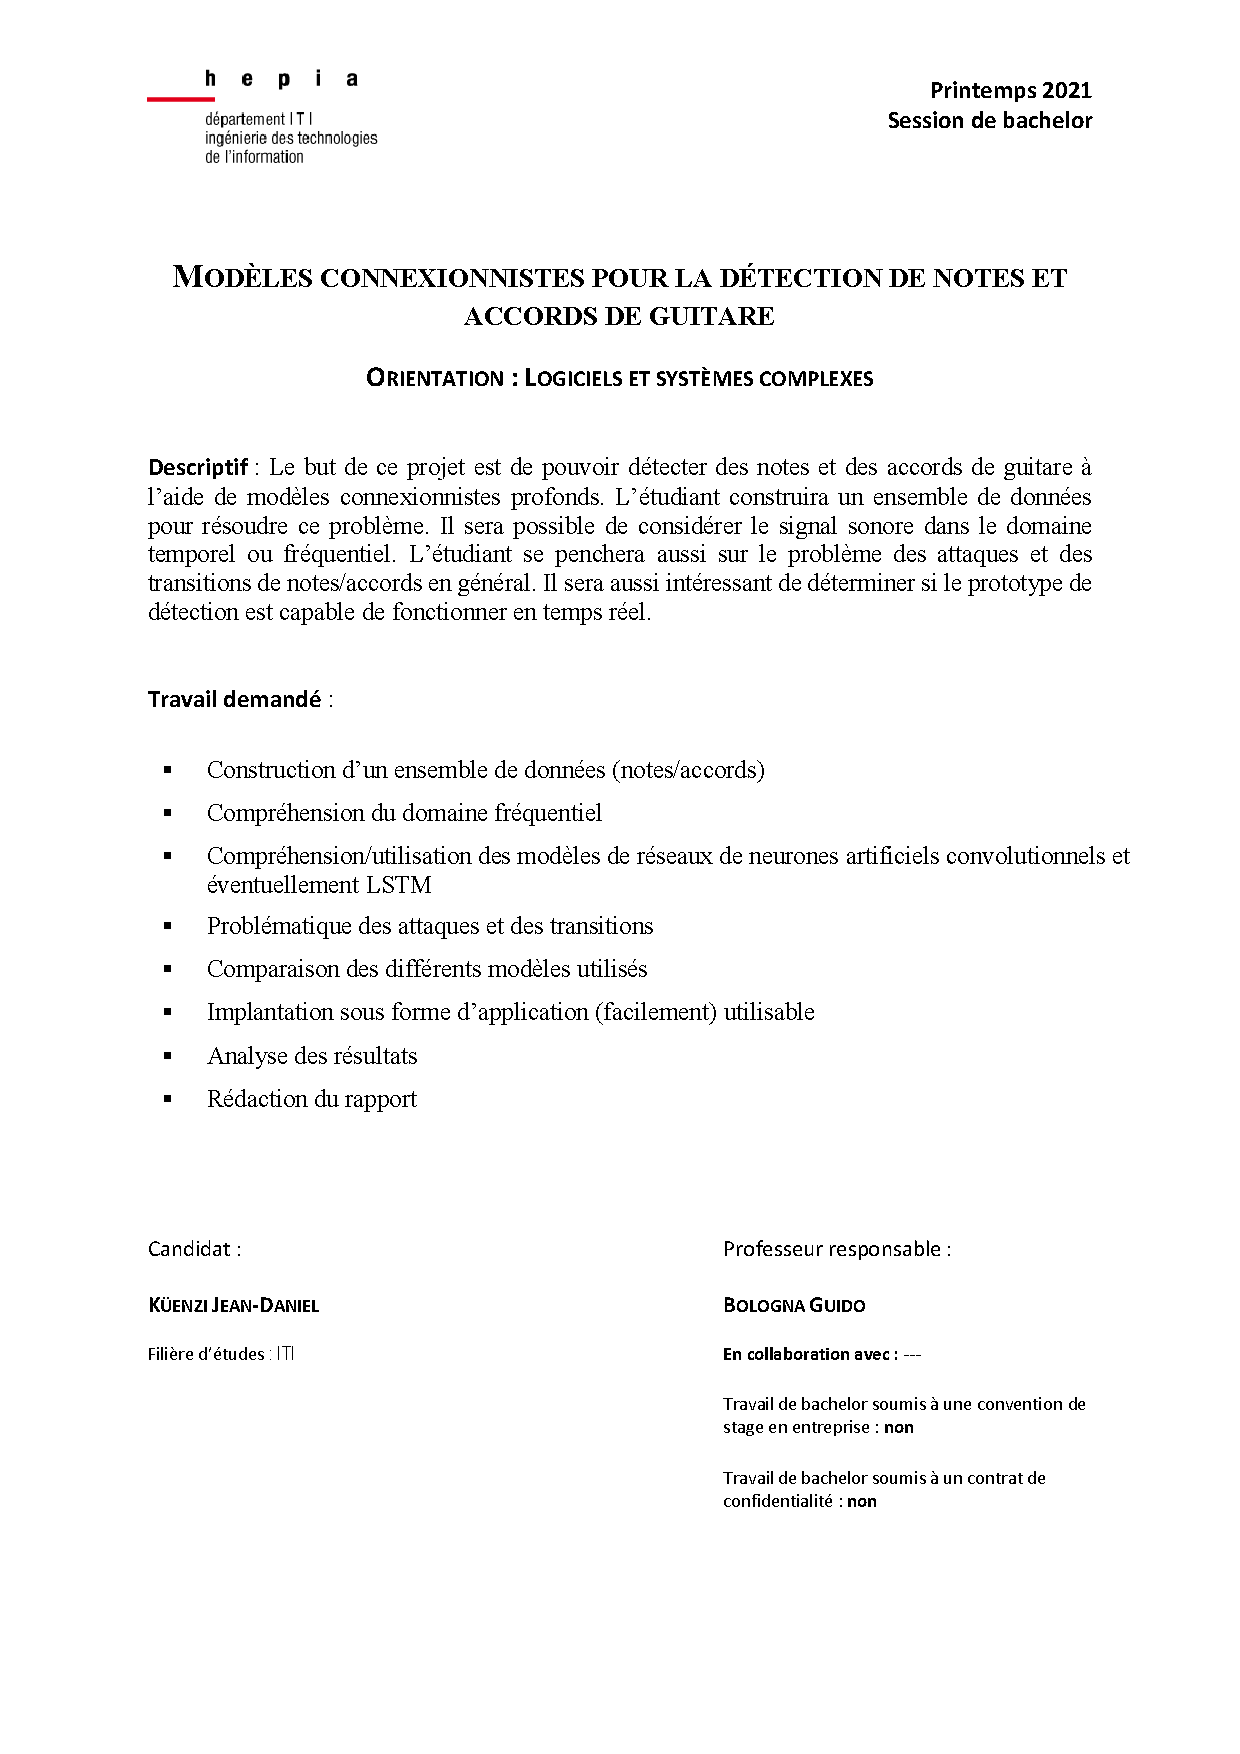
\includepdf[pages=-,pagecommand={\thispagestyle{noheader}}]{statements/statements.pdf}
%\clearpage
\cleardoublepage
%%%%%%%%%%%%%%%%%%%%%%%%%%%%%%%%%%%%%%% ABSTRACT %%%%%%%%%%%%%%%%%%%%%%%%%%%%%%%
%% !TeX spellcheck = fr_FR
%%%%%%%%%%%%%%%%%%%%%%%%%%%%%%%%%%%%%%%%%%%%%%%%%%%%%%%%%%%%%%%%%%%%%%%%%%%%%%%%
%%                                                                             %
%% HEPIA BACHELOR ABSTRACT LATEX TEMPLATE                                      %
%% version 0.10 - 2020/04/25                                                    %                                                                             %
%%                                                                             %
%%%%%%%%%%%%%%%%%%%%%%%%%%%%%%%%%%%%%%%%%%%%%%%%%%%%%%%%%%%%%%%%%%%%%%%%%%%%%%%%


%% To fill up by the student
\newcommand{\Session}{Printemps 2021}
\newcommand{\Author}{Küenzi Jean-Daniel}
\newcommand{\Professor}{Bologna Guido}
\newcommand{\Client}{---}
\newcommand{\Convention}{non}
\newcommand{\Confidentiel}{non}

\documentclass[12pt]
			{report}	% Set document to report class
\usepackage[T1]
			{fontenc}	% Font enconding
\usepackage[utf8]
			{inputenc}	% Set input encoding to utf-8, thus allow for non-ASCII characters
\usepackage[french]
			{babel}		% set document to default language to french
\usepackage[cm]
			{fullpage}	% Set margins to full page
\usepackage[a4paper,includehead,headheight=24pt,left=2.5cm, right=2.5cm, bottom=2.5cm, top=1.26cm]
			{geometry}	% Configure document geometry

\usepackage{tikz}		% Image and drawing related package
\usepackage{helvet}		% Helvetica font ~ Arial
\usepackage{mathptmx}	% Times font ~ Times New Roman


\usepackage[sfmath,notextcomp]{kpfonts} % Calibri replacement, font is \sf

\usepackage[scaled=0.85]
			{beramono}	% Vera mononspace {fvm}
\usepackage	{berasans}	% Vera sans {fvs}

%% This defines the default sans serif, roman and monospace fonts
\renewcommand{\sfdefault}
				{phv}	% helvetica as sans serif font
\renewcommand{\rmdefault}
				{ptm}	% times as roman (serif) font
\renewcommand{\ttdefault}
				{fvm}	% Vera mononspace as monospace font
\usepackage{bold-extra}	% Allow custom typsettings horrors like bold Small Caps
\usepackage{slantsc}	% Allow custom typsettings horrors like slanted Small Caps
\usepackage{numprint}	% number notation related package, e.g 10'000'000
\usepackage{setspace}	% linespacing related package


\usepackage{lipsum}		% Lorem Ipsum generator
%\usepackage{showframe}	% Print document frame


%%%%%%%%%%%%%%%%%%%%%%%%%%%%%%%%%%%% CUSTOM HEADER %%%%%%%%%%%%%%%%%%%%%%%%%%%%%
\usepackage{fancyhdr}
\pagestyle{fancy}
\renewcommand{\headrulewidth}{0pt}
\fancyhf{}
\fancypagestyle{plain}{
	\fancyhf{}%
	\fancyhead[L,C]{}
	\fancyhead[R]{\fontsize{11pt}{12.4pt} \sf \textbf{\\*\Session\\*[1.2pt]Session de bachelor}}
	\fancyfoot[L,C,R]{}
	\renewcommand{\headrulewidth}{0pt}
	\renewcommand{\footrulewidth}{0pt}
}
%%%%%%%%%%%%%%%%%%%%%%%%%%%%%%%% CUSTOM CHAPTER TITLES %%%%%%%%%%%%%%%%%%%%%%%%%
\usepackage{titlesec}
\titleformat{\chapter}[hang]{\centering \bfseries\scshape\Large}{\thechapter.}{1pc}{}
\titleformat{name=\chapter,numberless}[hang]{\fontsize{15.5}{18.7}\centering\bfseries\scshape}{}{1pc}{}
\titlespacing{\chapter}{0pt}{3em}{-12pt}
%\usepackage{showframe}	% Prints document frame

%%%%%%%%%%%%%%%%%%%%%%%%%%%%%%%%%%%%%%%%%%%%%%%%%%%%%%%%%%%%%%%%%%%%%%%%%%%%%%%%
%%%%%%%%%%%%%%%%%%%%%%%%%%%%%%%% DOCUMENT STARTS BELOW %%%%%%%%%%%%%%%%%%%%%%%%%
%%%%%%%%%%%%%%%%%%%%%%%%%%%%%%%%%%%%%%%%%%%%%%%%%%%%%%%%%%%%%%%%%%%%%%%%%%%%%%%%
\begin{document}
\chapter*{Résumé}
%% HEADER IMAGES
\tikz[remember picture,overlay] \node[shift={(4.655cm,-1.95cm)}] at (current page.north west)
{
\includegraphics[width=5.86cm,height=3.31cm]{template/images/title/hepia_logo}};
\begin{spacing}{0.956}
\vspace{0.5cm}

%% CONTENT STARTS HERE
Durant ces dernières années, l'Intelligence Artificielle (IA) n'a fait que progresser et a révolutionné beaucoup de domaines comme le droit, le domaine médical, la biologie ou encore la musique. Ce travail est la continuité de mon travail précédent, dont le but était de détecter des notes de trompette sur une octave de Do. L'objectif du présent travail est d'utiliser différentes architectures de modèle connexionniste (réseau neuronal) et de voir s'il est possible de détecter des notes et accords de guitare pour des sons mono échantillonnés à 44.1[kHz]. De plus, il sera possible de considérer le signal dans le monde discret (échantillonné) et dans le monde fréquentiel. Ainsi, le but est de parvenir à une utilisation en temps réel avec le moins de latence possible (autant visuelle qu'auditive). Dans le monde de la musique, une latence supérieure à cinq millisecondes pour le traitement du signal (calculs) est indésirable et se fait fortement ressentir. Le challenge est donc que les architectures proposées prédisent le plus précisément possible l'accord ou la note jouée dans un temps inférieur à cinq millisecondes. Pour ce travail, j'ai dû également créer un ensemble de données en partant de zéro. Par rapport au temps et aux ressources mises à ma disposition, j'ai décidé de m'attaquer à la gamme tempérée de la musique occidentale (pas de musique microtonale) et de représenter les accords mineurs et majeurs à trois sons et les notes dans leurs différentes octaves pour l'accordage standard d'une guitare (Mi, La, Ré, Sol, Si, Mi). L'architecture m'ayant donné les meilleurs résultats, à savoir une précision moyenne de 95.51\%, utilise une transformée de Fourier rapide pour passer dans le monde des fréquences et est composée d'une cellule LSTM bidirectionnelle.

\vfill
\begin{center}
	{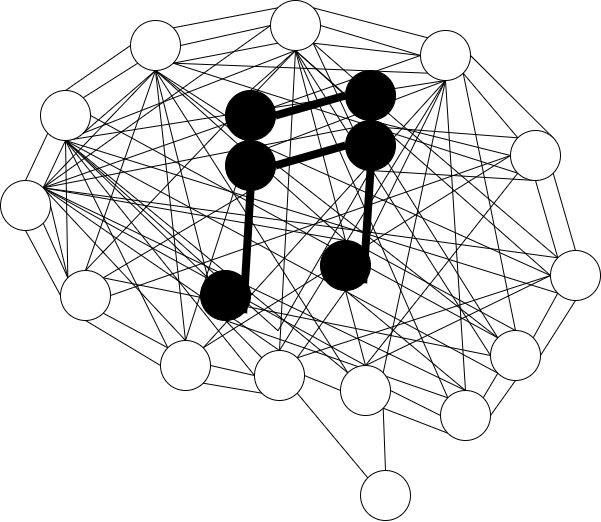
\includegraphics[height=5cm,width=5cm]{template/images/abstract/image}}\\*
\vfill
%% CONTENT ENDS HERE

\begin{center}
	{\sf
		%%%%%%%%%%%%%%%%%%%%%%%%%%%%%%%%%%%%%%%%%%%%%%%%%%%%%%%%%%%%%%%%%%%%%%%%%%%%%%%%
		%%%%%%%%%%%%%%%%%%%%%%%%%% DO NOT MODIFY THE TABLE BELOW %%%%%%%%%%%%%%%%%%%%%%%
		%%%%%%%%%%%%%%%%%%%%%%%%%%%%%%%%%%%%%%%%%%%%%%%%%%%%%%%%%%%%%%%%%%%%%%%%%%%%%%%%
		\begin{tabular*}{16cm}{p{7.7cm} p{7.7cm}}
			\small Candidat-e:					&	\small Professeur-e(s) responsable(s):\\*[10pt]
			\small\textbf{\textsc{\Author}}		&	\small\textbf{\textsc{\Professor}}\\*[10pt]
			\footnotesize  Filière d’études : ITI	&	\footnotesize  \textbf{En collaboration avec:} \textbf{\Client}\\*[10pt]
			\footnotesize  {} & \footnotesize  Travail de bachelor soumis à une convention de stage en entreprise: \textbf{\Convention}\\*[20pt]
			\footnotesize  {} & \footnotesize  Travail soumis à un contrat de confidentialité: \textbf{\Confidentiel}\\*[10pt]
		\end{tabular*}\\*[0.5cm]
	}
\end{center}

\end{center}
\end{spacing}
\end{document}

%\includepdf[pages=-,addtotoc={1,subsection,0,Résumé,abstract}]{../abstract/abstract.pdf}
\phantomsection
\addcontentsline{toc}{chapter}{Résumé}
\includepdf[pages=-,pagecommand={\thispagestyle{noheader}}]{abstract/abstract.pdf}
%\clearpage
\cleardoublepage
%%%%%%%%%%%%%%%%%%%%%%%%%%%%%%%%%%% LIST OF ACRONYMS  %%%%%%%%%%%%%%%%%%%%%%%%%%
% !TeX spellcheck = fr_FR
\printnoidxglossary[type=\acronymtype,nonumberlist,title={Liste des acronymes}]
% Use the acronyms
%\vspace{5cm}
%\textit{NB : Vous pouvez utiliser des acronymes en les définissant dans le fichier externe \texttt{/glossary/acronyms}. Une page dans la table des matières sera automatiquement ajoutée. Vous pourrez ensuite les référencer dans votre texte comme dans l'exemple ci-après:}\medskip

%\gls{utc} is 3 hours behind \gls{adt} and 10 hours ahead of \gls{est}.\medskip

%\textit{Lors de la première déclaration, l'acronyme est accompagné de sa définition, mais lors des utilisations suivantes, il ne l'est plus, comme illustré ci-dessous:}\medskip

%\gls{utc} is 3 hours behind \gls{adt} and 10 hours ahead of \gls{est}.
%\clearpage
\cleardoublepage
%%%%%%%%%%%%%%%%%%%%%%%%%%%%%%%%%%% LIST OF FIGURES %%%%%%%%%%%%%%%%%%%%%%%%%%%%
% !TeX spellcheck = fr_FR
\renewcommand{\listfigurename}{Liste des illustrations}
\listoffigures
\addcontentsline{toc}{chapter}{\listfigurename} % Adding toc entry

\paragraph{Références des URL}

\begin{itemize}
\item URL01\quad\href{https://fr.wikipedia.org/wiki/\%C3\%89chelle\_chromatique}{https://fr.wikipedia.org/wiki/Échelle\_chromatique}
\item URL02\quad\href{https://pythonmachinelearning.pro/perceptrons-the-first-neural-networks/}{https://pythonmachinelearning.pro/perceptrons-the-first-neural-networks/}
\item URL03\quad\href{https://fr.wikipedia.org/wiki/Fonction\_d\%27activation}{https://fr.wikipedia.org/wiki/Fonction\_d'activation}
\item URL04\quad\href{https://medium.com/@temi.ayo.babs/multi-layer-perceptron-for-beginners-6aee246c6a03}{https://medium.com/@temi.ayo.babs/multi-layer-perceptron-for-beginners-6aee246c6a03}
\item URL05\quad\href{https://medium.com/analytics-vidhya/from-convolutional-neural-network-to-variational-auto-encoder-97694e86bb51 }{https://medium.com/analytics-vidhya/from-convolutional-neural-network-to-variational-auto-encoder-97694e86bb51 }
\item URL06\quad\href{https://ai.plainenglish.io/pooling-layer-beginner-to-intermediate-fa0dbdce80eb}{https://ai.plainenglish.io/pooling-layer-beginner-to-intermediate-fa0dbdce80eb}
\item URL07\quad\href{https://www.kdnuggets.com/2016/11/intuitive-explanation-convolutional-neural-networks.html/3}{https://www.kdnuggets.com/2016/11/intuitive-explanation-convolutional-neural-networks.html/3}
\item URL08\quad\href{https://towardsdatascience.com/softmax-activation-function-explained-a7e1bc3ad60}{https://towardsdatascience.com/softmax-activation-function-explained-a7e1bc3ad60}
\item URL09\quad\href{http://apmonitor.com/do/index.php/Main/LSTMNetwork}{http://apmonitor.com/do/index.php/Main/LSTMNetwork}
\item URL10\quad\href{https://fr.mathworks.com/help/dsp/ref/dsp.stft.html}{https://fr.mathworks.com/help/dsp/ref/dsp.stft.html}
\end{itemize}
%\clearpage
\cleardoublepage
%%%%%%%%%%%%%%%%%%%%%%%%%%%%%%%%%%%% LIST OF TABLES %%%%%%%%%%%%%%%%%%%%%%%%%%%%
% !TeX spellcheck = fr_FR
\renewcommand{\listtablename}{Liste des tableaux}
\listoftables
\addcontentsline{toc}{chapter}{\listtablename} % Adding toc entry

%\vspace*{14.4pt}

%\textit{N.B. Si vous avez peu de tableaux, vous pouvez les intégrer à la table des illustrations.}

%\vspace*{14.4pt}

\paragraph{Références des URL}

\begin{itemize}
\item URL11\quad\href{https://fr.wikipedia.org/wiki/Note_de_musique}{https://fr.wikipedia.org/wiki/Note\_de\_musique}
\end{itemize}
\end{spacing}
%\clearpage
\cleardoublepage
%%%%%%%%%%%%%%%%%%%%%%%%%%%%%%%%%%% LIST OF ANNEXES %%%%%%%%%%%%%%%%%%%%%%%%%%%%
%%% COMMENT THIS PART IF YOU DO NOT USE DEDICATED TOC FOR ANNEXES AND COMMENT 
%%% HEADER AND FOOTER PART IN {chapters/annexes} FILE
\begin{spacing}{1}
% !TeX spellcheck = fr_FR
\chapter*{Liste des annexes} % No (numbered) toc entry with *
\addcontentsline{toc}{chapter}{Liste des annexes} % Adding toc entry

\printcontents[annexes]{ }{2}{}
\end{spacing}
%\clearpage
\cleardoublepage
%%%%%%%%%%%%%%%%%%%%%%%%%%%%%%%%%%%%% INTRODUCTION  %%%%%%%%%%%%%%%%%%%%%%%%%%%%
\begin{spacing}{1.5}
\pagenumbering{arabic}
% !TeX spellcheck = fr_FR
\chapter*{Introduction}
\addcontentsline{toc}{chapter}{Introduction} % Adding toc entry

L’\gls{ia} a révolutionné bien des domaines lors des décennies passées. Même en musique, l’\gls{ia} est désormais omniprésente, allant du simple filtre à la composition de morceau\footnote{\url{https://www.aiva.ai/}}. Généralement, ses applications sont définies pour le monde professionnel, mais avec l'explosion des technologies de l'information et l'accessibilité des données, beaucoup de personnes s'intéressent au monde de la musique de manière autodidacte. Étant moi-même de base autodidacte, j'ai beaucoup appris en écoutant des morceaux et en essayant de reproduire les accords. Toutefois, je me rendais compte que même si j'arrivais à reproduire les accords à l'oreille, je ne connaissais ni leurs noms ni leurs formes (majeure, mineure, etc.). En discutant avec mon prof de musique, il m'a fait part de la même constatation chez certains de ses élèves. C'est pourquoi j'ai eu l'idée de faire une \gls{ia} capable de reconnaitre des notes et accords de guitare, ainsi, il est possible pour les personnes autodidactes d'avoir plus de facilité à comprendre la structure d'un morceau ou d'une gamme.

Ce travail est la continuité de mon travail précédent, dont le but était de détecter des notes de trompette sur une octave de Do. L'objectif de cette nouvelle étude est d'utiliser différentes architectures de modèle connexionniste (réseau neuronal) et de voir s'il est possible de détecter des notes et accords de guitare pour des sons mono échantillonnés à 44.1[kHz]. De plus il sera possible de considérer le signal dans le monde discret (échantillonné) et dans le monde fréquentiel. L’objectif est ainsi d’arriver à une utilisation en temps réel avec le moins de latence possible (visuelle et auditive). Dans le monde de la musique, une latence supérieure à cinq millisecondes pour le traitement du signal (calculs) est indésirable et se fait fortement ressentir. Le challenge est donc que les architectures proposées prédisent le plus précisément possible l'accord ou la note jouée et tout ça dans un temps inférieur à cinq millisecondes. Bien sûr, comme il n'est pas possible de faire du temps réel en informatique, l'objectif sera d'utiliser un temps d'échantillonnage suffisamment court (moins d'un dixième de seconde) afin de ne pas ressentir le temps de latence.

Pour ce travail, j'ai dû également créer un ensemble de données en partant de zéro. Par rapport au temps et aux ressources mises à ma disposition, j'ai décidé de m'attaquer à la gamme tempérée de la musique occidentale (pas de musique microtonale) et de représenter les accords mineurs et majeurs à trois sons dans l'accordage standard d'une guitare (Mi, La, Ré, Sol, Si, Mi). Ces accords seront joués jusqu'à la $12^{\text{ème}}$ frette (case de la guitare) non incluse et sur les deux cordes les plus graves, à savoir Mi et La. Quant aux notes, elles sont toutes représentées dans leurs différentes octaves et positions, toujours par rapport à l'accordage standard.

Les premières semaines de travail m'ont servi à récolter un maximum d'informations sur les solutions similaires existantes (traitement de la voix, détection de clés, etc.) et à comprendre les notions mathématiques nécessaires à la réalisation du travail. Pour les notions mathématiques je me suis basé sur un cours de $3^{\text{ème}}$ année à l'École Nationale Supérieure de l'Électronique et de ses Applications (ENSEA) sur le traitement de signal \parencite{peeters_ensea_2017} présenté par le professeur Geoffroy \textsc{Peeters}. Il est chercheur à l’Institut de Recherche et Coordination Acoustique/Musique (IRCAM) où il supervise notamment les travaux de Master et de Doctorat.

Durant ces premières semaines, j'ai aussi profité de mettre en place un environnement virtuel Conda\footnote{\url{https://conda.io/projects/conda/en/latest/index.html}} afin de bénéficier d'un environnement de travail dans lequel je pourrais utiliser les API d'apprentissage profond.

Étant familier avec l'API d'apprentissage profond Keras\footnote{\url{https://keras.io/}} (API de Google), j'ai commencé à développer de petits réseaux de neurones afin de bien comprendre comment fonctionnent les cellules LSTM que je n'avais jusqu'alors pas réellement explorées. Toutefois, Keras est une API assez haut niveau qui restreint un peu l'utilisateur, c'est pourquoi j'ai décidé de partir sur PyTorch\footnote{\url{https://pytorch.org/}} (API de Facebook) qui est plus bas niveau, donc plus difficile à utiliser, mais qui me permettait d'être plus libre, surtout sur la création de couches personnalisées et les architectures de mes modèles. J'ai donc dû lire la documentation PyTorch et dû effectuer quelques expérimentations pour apprendre à utiliser correctement cette nouvelle API.

Durant mon apprentissage de l'API PyTorch, j'ai aussi pu examiner les modèles proposés par la communauté PyTorch et notamment ceux qui sont en lien avec le monde de la musique comme OPEN-UNMIX\footnote{\url{https://github.com/sigsep/open-unmix-pytorch}}. Ces modèles sont généralement bien documentés et m'ont permis d'acquérir et de comprendre des nouvelles bases comme les skip-layer, la normalisation par lots ou encore les cellules LSTM bidirectionnelles. Pour ces nouvelles connaissances, je me suis basé sur des études pour la plupart disponibles sur la plateforme arXiv\footnote{\url{https://arxiv.org/}} (plateforme d'archives de prépublication scientifique) qui m'ont permis de comprendre l'essentiel des informations. Elles ont aussi servi à renforcer mes bases déjà acquises et à me rendre plus confiant quant à mes choix.

Je suis ensuite passé à une phase d'expérimentation pendant laquelle j'ai testé plusieurs types d'architectures pour mes modèles connexionnistes, différentes tailles de fenêtres (temps d'échantillonnage) et différentes techniques de traitement du signal. J'ai notamment aussi enregistré deux ensembles de données, l'un avec une carte son interne à mon ordinateur et l'autre avec une carte son externe spécialisée dans le traitement audio.

Afin de sauvegarder mon travail, j'ai créé un répertoire Git\footnote{\url{https://gitedu.hesge.ch/jeandani.kuenzi/bachelor.git}} sur lequel se trouve mon ensemble de données, ma thèse au format PDF ainsi qu'au format LaTeX, les images présentes dans cette thèse, le code ayant servi à entrainer et créer mes différentes architectures ainsi que mon environnement Conda au format YAML.

Au cours de cette thèse, nous verrons tout d'abord les solutions existantes que j'ai retenues et nous les détaillerons un peu.

Puis, nous verrons les notions théoriques nécessaires à la bonne compréhension du travail. Il y aura tout d'abord les notions musicales qui expliqueront ce que c'est qu'un son, comment est composé un accord et comment différencier un accord majeur d'un accord mineur.

Ensuite, il y aura une partie sur les notions mathématiques afin de bien comprendre comment on représente un son dans le monde fréquentiel et comment on passe du monde discret au monde fréquentiel ainsi que les différents problèmes qui peuvent y survenir.

Nous verrons également les notions nécessaires à la bonne compréhension de ce qu'est un réseau de neurones et comment il fonctionne depuis sa base qui est le Perceptron.

Je parlerai également de la manière dont j'ai créé mon ensemble de données, la structure des fichiers audio que j'ai enregistrés, le matériel utilisé et les différentes techniques que j'utilise dans le prétraitement de celui-ci.

Ensuite, j'expliquerai ma solution ainsi que les différentes parties qui la composent. Je vais notamment dans cette partie justifier mon choix concernant l'architecture de cette dernière.

Après cela, je présenterai sans rentrer dans le détail les architectures que j'ai testées durant mes expérimentations et que je n'ai pas retenues.

Finalement, je présenterai et débattrai des différents résultats obtenus avec ma solution et j'expliquerai également mon ressentiment d'utilisation en temps réel.
%\clearpage
\cleardoublepage
%%%%%%%%%%%%%%%%%%%%%%%%%%%%%%%%%%%%%%% CHAPTERS %%%%%%%%%%%%%%%%%%%%%%%%%%%%%%%
%%%%%%%%%%%%%%%%%%%%%%%%%%%%%%% Add your chapters here %%%%%%%%%%%%%%%%%%%%%%%%%
%\input{chapters/chapXXX}
% !TeX spellcheck = fr_FR
\chapter{Chapitre 1 : Analyse de l'existant}
\label{chap:1}

Lors de mes recherches de solutions similaires, j'ai notamment retenu deux travaux utilisant des réseaux de neurones afin de détecter en temps réel des accords de guitare, Chord AI\footnote{\url{https://www.chordai.net/}} et Uberchord\footnote{\url{https://www.uberchord.com/}}. L'un deux a été développé en collaboration avec l'\gls{epfl}.

\section{Chord AI}
\label{sec:1.1}

Chord AI est une application Android et iOS qui a été développée par Vivien \textsc{Seguy}\footnote{\url{https://vivienseguy.github.io/}}, le CEO de Nomad AI\footnote{\url{https://www.nomadai.org/}}, avec la collaboration de Guillaume \textsc{Bellec}\footnote{\url{http://guillaume.bellec.eu/}}, un chercheur postdoctorant à l'\gls{epfl}. Lors de sa création, l'application était capable de reconnaitre les accords majeurs et mineurs. À ce jour, elle a été améliorée et est maintenant capable de reconnaitre plus de 500 accords sans compter les inversions. Elle propose aussi une reconnaissance de clés basée sur les accords détectés. Toutefois, elle n'est pas capable de reconnaitre les notes de musique.

J'ai notamment pu tester l'application et lors de mon utilisation, j'ai constaté qu'elle enregistrait en temps réel ce que je jouais mais qu'il y avait un décalage de \textasciitilde$1/2$[s] entre le moment où je jouais l'accord et la prédiction de celui-ci. Afin de comprendre pourquoi ce décalage avait lieu, j'ai contacté Vivien \textsc{Seguy} et il a accepté de s'entretenir avec moi afin de discuter du fonctionnement de l'application. Il m'a expliqué qu'elle utilise un \gls{rnr} pour la prédiction des accords et que la taille des fenêtres utilisée est de \textasciitilde$0.4$[s] échantillonnée à 22.05[kHz]. Ce qui représente à peu près une fenêtre de $8820$ échantillons. Les différentes fenêtres se chevauchent de \textasciitilde$0.2$[s]. Une \gls{tfct} va être appliquée sur la fenêtre lors du prétraitement ce qui va nous créer une image 2D, qu'on appel un spectrogramme. Cette image traversera un petit \gls{rnc} avant de traverser le \gls{rnr} afin de faire la prédiction de l'accord.

\section{Uberchord}
\label{sec:1.2}

Uberchord est une application iOS qui permet d'apprendre à jouer de la guitare de manière autodidacte. Elle propose notamment un système de suivi personnalisé en temps réel entièrement géré par une \gls{ia}. Elle possède aussi une fonctionnalité de détection d'accords en temps réel. L'\gls{ia} serait apparemment capable de prédire n'importe quels accords en temps réel et dans 19 accordages de guitare différents. Toutefois, il ne semble pas y avoir de fonctionnalité capable de reconnaitre les notes de musique.
% !TeX spellcheck = fr_FR
\chapter{Chapitre 2 : Notions musicales}
\label{chap:2}

\section{La gamme tempérée}
\label{sec:2.1}

La gamme tempérée ou à tempérament égal est en musique occidentale une gamme qui divise une octave en douze parties sur une échelle logarithmique avec un rapport égal à $\sqrt[12]{2}$. Pour passer à la note suivante, on multiplie la fréquence par $\sqrt[12]{2}$. Et donc inversement, pour passer à la note précédente on divise la fréquence par $\sqrt[12]{2}$.

\begin{figure}[H]
	\centering
	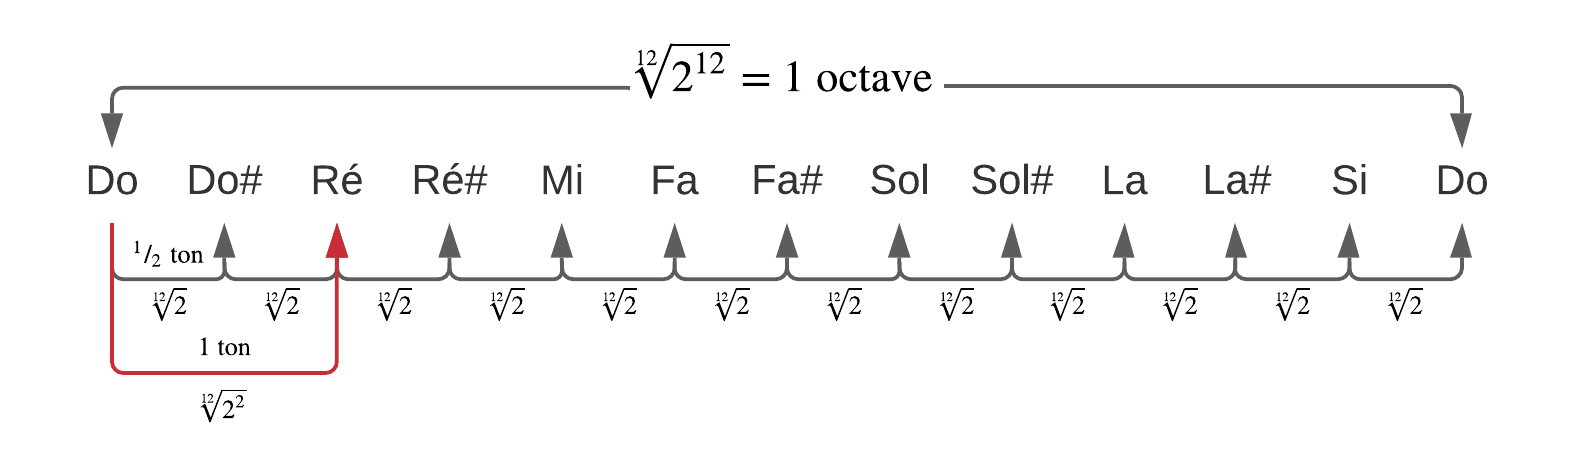
\includegraphics[width=1\linewidth]{gamme_temp}
	\caption[Gamme tempérée]{Gamme tempérée. Source : Réalisé par \textsc{Küenzi} Jean-Daniel}
	\label{fig:gammetemp}
\end{figure}

\section{Les notes de la gamme tempérée}
\label{sec:2.2}

\begin{table}[H]
	\centering{
		\begin{tabular}{|c|c|}
			\hline
			\textbf{Notation anglophone} & \textbf{Notation latine} \\
			\hline
			C & Do \\
			\hline
			C\sh\hspace{2pt}ou D\fl & Do\sh\hspace{2pt}ou Ré\fl \\
			\hline
			D & Ré \\
			\hline
			D\sh\hspace{2pt}ou E\fl & Ré\sh\hspace{2pt}ou Mi\fl \\
			\hline
			E & Mi \\
			\hline
			F & Fa \\
			\hline
			F\sh\hspace{2pt}ou G\fl & Fa\sh\hspace{2pt}ou Sol\fl \\
			\hline
			G & Sol \\
			\hline
			G\sh\hspace{2pt}ou A\fl & Sol\sh\hspace{2pt}ou La\fl \\
			\hline
			A & La \\
			\hline
			A\sh\hspace{2pt}ou B\fl & La\sh\hspace{2pt}ou Si\fl \\
			\hline
			B & Si \\
			\hline 
		\end{tabular}
		\caption[Notes de musique occidentale]{Notes de musiques occidentale. Source : Réalisé par \textsc{Küenzi} Jean-Daniel}
		\label{tab:notes}
	}
\end{table}

Dans cette thèse, nous utiliserons la notation anglophone pour représenter les notes et accords de musique.

\subsection{Explication des dièses (\#) et bémols ($\flat$)}

Dans la musique occidentale, les \# et $\flat$ permettent de représenter les altérations de la hauteur naturelle de la note visée. \# la note est élevée d'un demi-ton, $\flat$ la note est abaissée d'un demi-ton.

\begin{figure}[H]
	\centering
	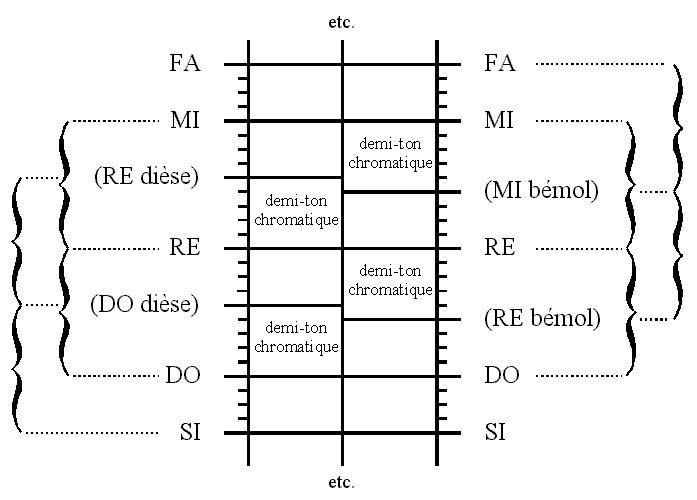
\includegraphics[width=0.7\linewidth]{chroma_ladder}
	\caption[Échelle chromatique]{Échelle chromatique. Source : tiré de \textit{Wikipedia}, ref. URL01}
	\label{fig:chroma_ladder}
\end{figure}

\section{Construction d'un accord à trois sons}
\label{sec:2.3}

En harmonie tonale, un accord à trois sons est composé : d'une fondamentale, d'une tierce qui peut être mineure ou majeure et d'une quinte qui peut être juste, augmentée ou diminuée. Ce qui différencie un accord majeur d'un accord mineur est donc sa tierce.

Dans cette thèse nous verrons uniquement les accords à trois sons dit "parfaits". C'est-à-dire que leur quinte est juste.

\subsection{Majeur}
La construction d'un accord parfait majeur est très simple. Il y a tout d'abord la fondamentale qui va être notre note de base sur laquelle se construit notre accord. Puis la tierce qui est donc majeure, cela veut dire qu'elle se trouve à deux tons de la fondamentale. Puis la quinte qui est juste et se trouve donc à trois tons et demi de la fondamentale.

Prenons comme exemple l'accord AMaj (La Majeur). Il a comme fondamentale A. Puis la tierce majeure qui se trouve à deux tons de la fondamentale, c'est à dire C\sh. Pour finir la quinte juste qui se trouve à trois tons et demi de la fondamentale, c'est à dire E. Notre accord AMaj est donc construit de la manière suivante :

\begin{table}[H]
	\centering{
		\begin{tabular}{|l|c|c|}
			\hline
			\multicolumn{3}{|c|}{\textbf{A Majeur}} \\
			\hline
			& \textbf{Notes} & \textbf{Ton(s)} \\
			\hline
			Fondamentale & A & $\emptyset$ \\
			\hline
			Tierce majeure & C\sh & 2 \\
			\hline
			Quinte juste & E & 3.5 \\
			\hline 
		\end{tabular}
		\caption[Construction de l'accord AMaj]{Construction de l'accord AMaj. Source : Réalisé par \textsc{Küenzi} Jean-Daniel}
		\label{tab:amaj}
	}
\end{table}

\subsection{Mineur}

La construction d'un accord parfait mineur est très simple. Il y a tout d'abord la fondamentale qui va être notre note de base sur laquelle se construit notre accord. Puis la tierce qui est donc mineure. Cela veut dire qu'elle se trouve à un ton et demi de la fondamentale. Puis la quinte qui est juste et se trouve donc à trois tons et demi de la fondamentale.

Prenons comme exemple l'accord Amin (La mineur). Il a comme fondamentale A. Puis la tierce qui doit être mineure et qui se trouve donc à un ton et demi de la fondamentale, c'est à dire C. Pour finir la quinte est juste, elle se trouve donc à trois tons et demi de la fondamentale, c'est à dire E (comme pour AMaj). Notre accord Amin est donc construit de la manière suivante :

\begin{table}[H]
	\centering{
		\begin{tabular}{|l|c|c|}
			\hline
			\multicolumn{3}{|c|}{\textbf{A mineur}} \\
			\hline
			& \textbf{Notes} & \textbf{Ton(s)} \\
			\hline
			Fondamentale & A & $\emptyset$ \\
			\hline
			Tierce mineure & C & 1.5 \\
			\hline
			Quinte juste & E & 3.5 \\
			\hline 
		\end{tabular}
		\caption[Construction de l'accord Amin]{Construction de l'accord Amin. Source : Réalisé par \textsc{Küenzi} Jean-Daniel}
		\label{tab:amin}
	}
\end{table}

\section{Attaque d'une note ou d'un accord}
\label{sec:2.4}

En acoustique, l'attaque est la façon de commencer/jouer une note ou un accord sur un instrument. L'attaque va être un problème dans ce travail, car elle contient beaucoup d'informations (bruit) et se trouve au début de la note, elle va donc fausser l'apprentissage et les résultats prédits. Nous verrons dans le \autoref{chap:4} ce que j'ai mis en place afin d'y pallier.

\section{Transformée de Fourier Discrète (TFD)}
\label{sec:2.5}

La \gls{tfd} sert essentiellement à transformer un signal discret (échantillonné) en une représentation spectrale discrète. L’échantillonnage est fait sur une fenêtre d’analyse bornée dans le temps. La \gls{tfd} va décomposer notre signal en plusieurs superpositions d'ondes sinusoïdales de fréquences différentes. C’est donc un équivalent à la \gls{tf}, mais dans le monde discret et pour les signaux non périodiques. Avec un signal discret $y$ et un nombre d’échantillons $N$, la \gls{tfd} peut être définie comme

{\Large
	\setlength{\abovedisplayskip}{-0.5cm}
	\begin{align*}
			y[k] = \sum_{n=0}^{N-1}{y[n] * \text{exp}(-\frac{2i\pi}{N}kn)} \text{\hspace{10pt}avec 0 $\leq$ k < N}
	\end{align*}
}

\section{Transformée de Fourier Rapide (TFR)}
\label{sec:2.6}

La \gls{tfr} est un algorithme de calculs utilisant la \gls{tfd}. La \gls{tfr} améliore la complexité de la \gls{tfd} $O(N^{2})$, où $N$ est le nombre d’échantillons, en la réduisant à $O(N log N)$ à l’aide de la factorisation matricielle et de divisions du problème en plusieurs parties (diviser pour régner).

\section{Fenêtre de Hamming}
\label{sec:2.7}

Lorsque nous voulons analyser un signal avec une \gls{tfd} ou une \gls{tfr}, on devrait théoriquement connaitre la période du signal que l'on veut analyser. En pratique on ne connait pas toujours cette période. La fenêtre va nous être utile pour éviter la fuite spectrale. La fuite spectrale est un phénomène qui survient lorsque l'on passe à la \gls{tfd} un signal avec une période incomplète. Par exemple pour le A à 220[Hz], examinons son spectre de Fourier sans utiliser une fenêtre de Hamming.

\begin{figure}[H]
	\centering
	\includegraphics[width=1\linewidth]{fft_a220_no_hamming}
	\caption[Spectre de Fourier d'un A à 220 Hertz (fuite spectrale)]{Spectre de Fourier d'un A à 220[Hz] (Fuite spectrale). Source : Réalisé par \textsc{Küenzi} Jean-Daniel}
	\label{fig:fft_a220_no_hamming}
\end{figure}

Comme on peut le voir, la \gls{tfr} nous montre que notre signal est composé de plusieurs sinus autour de 220[Hz]. Or ce n'est pas très juste, même si en pratique il y a toujours du bruit et des interférences, on s'attendrait plutôt à obtenir un spectre plus précis, surtout autour de la fréquence fondamentale. C'est là que la fenêtre de Hamming va nous aider. En multipliant notre signal par cette fenêtre, nous allons réduire la fuite spectrale. Toutefois, on ne peut que la réduire et non l'annuler. Avec un signal $x$, un nombre d'échantillons $N$, la fenêtre de Hamming peut être définie comme

{\Large
	\setlength{\abovedisplayskip}{-0.5cm}
	\begin{align*}
		x[n] = 0.54 - 0.46 \cos(2\pi\frac{n}{N})
	\end{align*}
}

\begin{figure}[H]
	\centering
	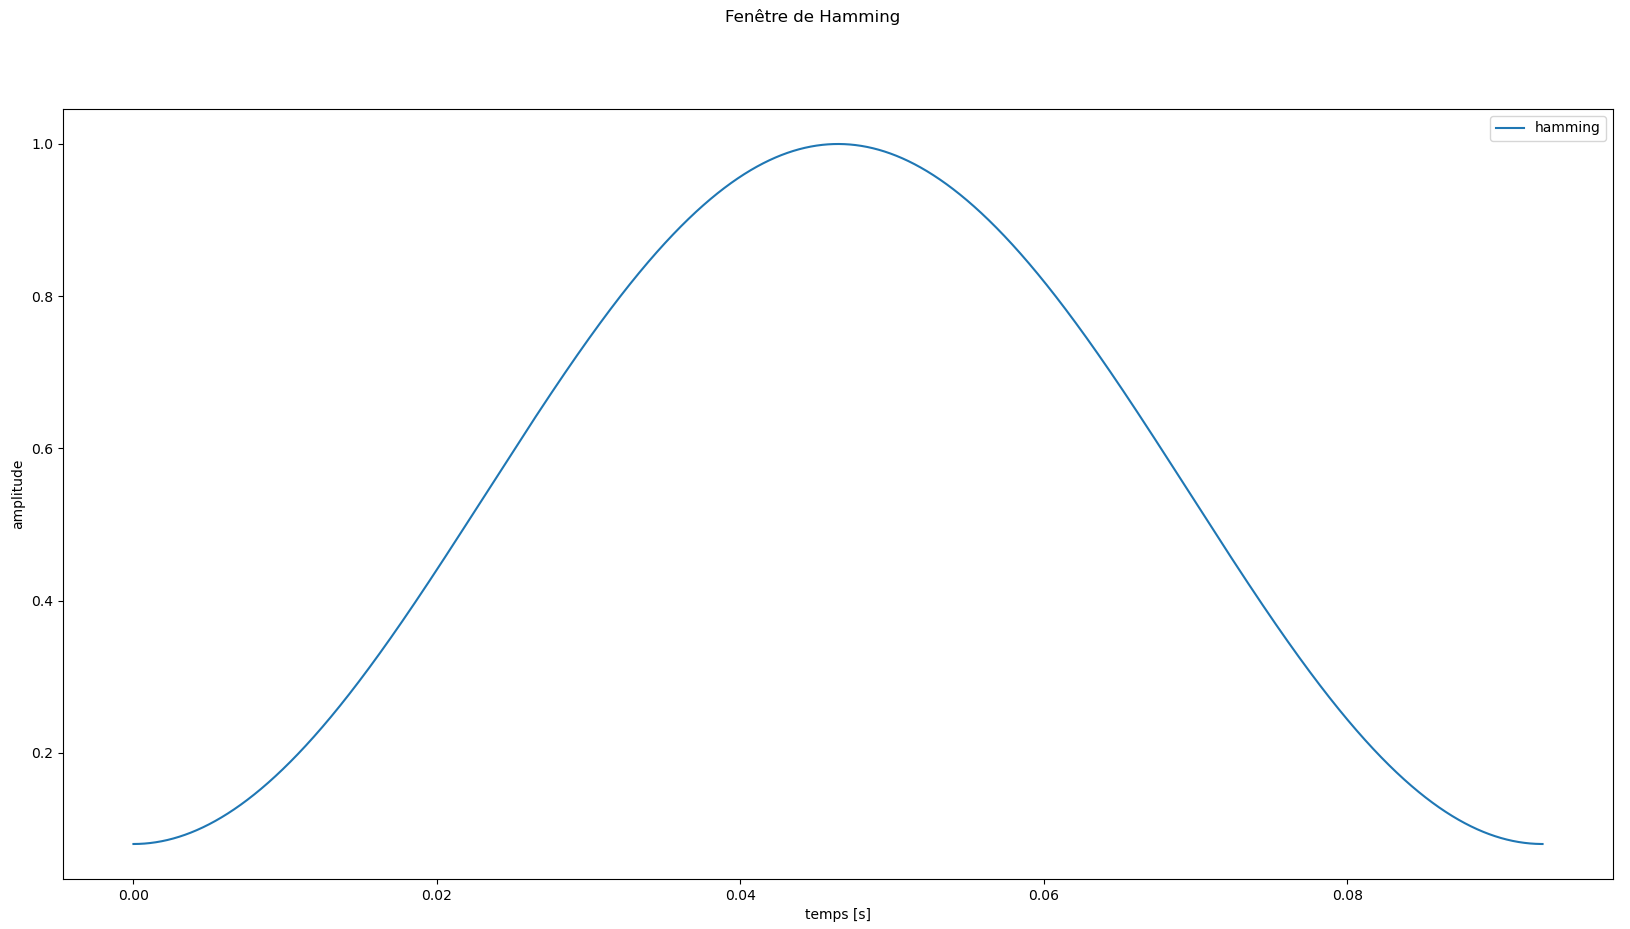
\includegraphics[width=1\linewidth]{hamming_window}
	\caption[Fenêtre de Hamming]{Fenêtre de Hamming. Source : Réalisé par \textsc{Küenzi} Jean-Daniel}
	\label{fig:hamming_window}
\end{figure}

\section{Partiel harmonique}
\label{sec:2.8}

"En acoustique, un partiel harmonique est une composante d’un son périodique, dont la fréquence est un multiple entier d'une fréquence fondamentale." \parencite{noauthor_harmonique_2021}. On peut visualiser les partiels harmoniques d'un signal en affichant son spectre de Fourier. Mais comme la \gls{tfd} se passe dans le monde des nombres complexes, ce que l'on va tracer sur notre spectre est le module de ses nombres. Avec un nombre complexe $z$, la partie réelle $a$ et la partie imaginaire $b$, le module peut être décrit comme

{\Large
	\setlength{\abovedisplayskip}{-0.5cm}
	\begin{align*}
		\lvert z\rvert = \sqrt{a^2 + b^2}
	\end{align*}
}

\subsection{Partiels harmoniques d'une note}

Par exemple pour un A à 220 [Hz] qui est échantillonné à 44.1[kHz] sur une fenêtre de 4096 échantillons, ce qui correspond à une résolution temporelle de \textasciitilde0.093[s], si l'on analyse son spectre de Fourier à l’aide d’une \gls{tfr}, on obtient le spectre suivant

\begin{figure}[H]
	\centering
	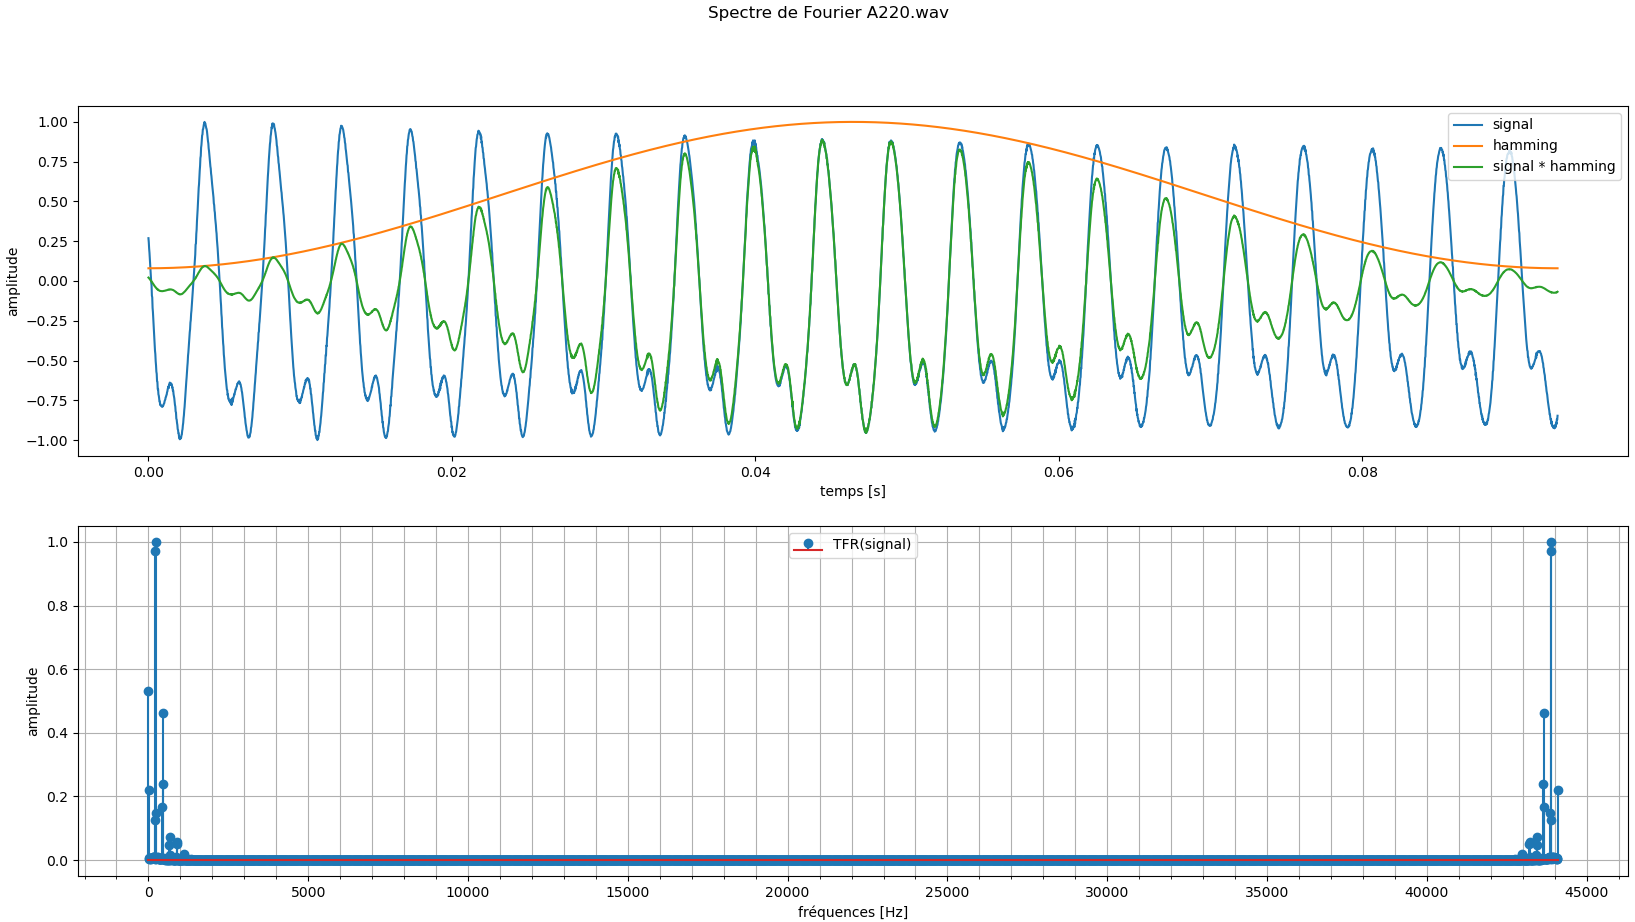
\includegraphics[width=1\linewidth]{fft_total_A220}
	\caption[Spectre de Fourier d'un A à 220 Hertz (entier)]{Spectre de Fourier d'un A à 220[Hz] (entier). Source : Réalisé par \textsc{Küenzi} Jean-Daniel}
	\label{fig:fft_total_a220}
\end{figure}

On ne voit pas grand-chose, mais on peut remarquer tout de même une sorte de symétrie. En fait les fréquences qui se trouvent à droite sont appelées les conjugués des coefficients de Fourier et elles se trouvent après la fréquence de Nyquist. La fréquence de Nyquist est égale à la moitié de la fréquence d'échantillonnage, donc dans notre cas 22.05[kHz]. Mais ce qui nous intéresse est le spectre continu du signal, c'est-à-dire la partie avec les fréquences à gauche. On va donc observer ce qui se passe entre la bande de fréquences [0;1'000] Hertz.

\begin{figure}[H]
	\centering
	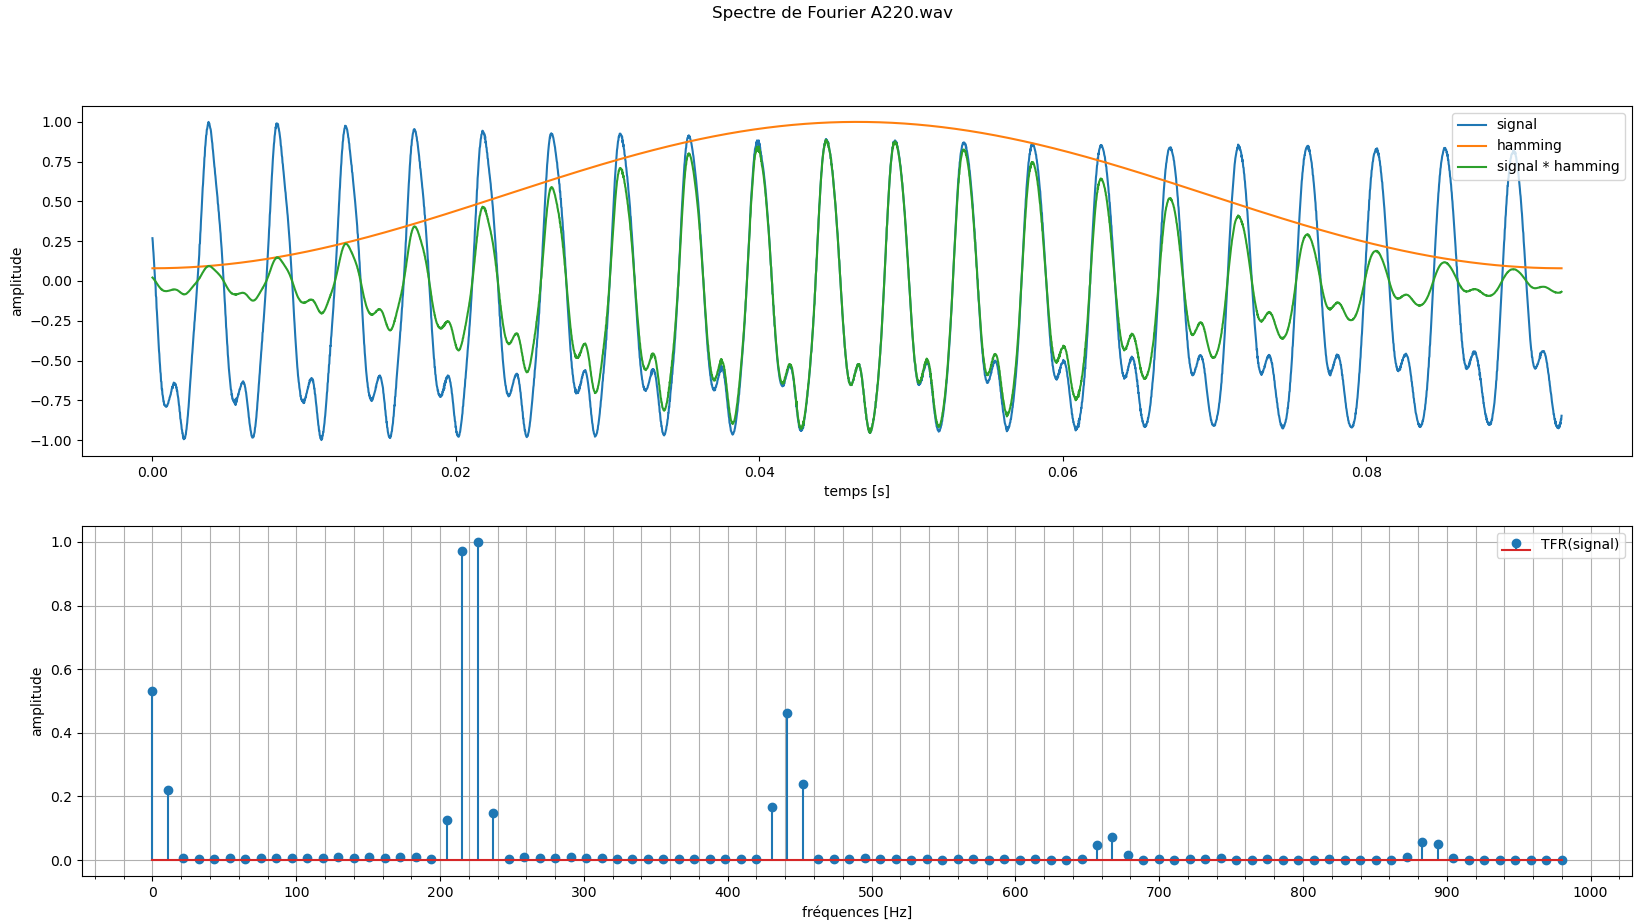
\includegraphics[width=1\linewidth]{fft_A220}
	\caption[Spectre de Fourier d'un A à 220 Hertz (spectre continu)]{Spectre de Fourier d'un A à 220[Hz] (spectre continu). Source : Réalisé par \textsc{Küenzi} Jean-Daniel}
	\label{fig:fft_a220}
\end{figure}

On remarque tout d'abord un pic à zéro. Ce pic correspond à ce qu'on appelle la fréquence nulle. Ensuite, on voit qu’il y a deux pics autour de 220[Hz], ce qui correspond donc à notre fréquence fondamentale, puis un autre pic à 440[Hz] qui correspond donc au premier partiel harmonique $2f_{1}$, puis un troisième à $3f_{1}$, etc. Le spectre de Fourier n'est pas très précis, mais cela s'explique par le fait que nous avons une résolution fréquentielle (précision) de \textasciitilde$10.77$[Hz]. Avec $f_{e}$ la fréquence d'échantillonnage et $n$ la taille de notre fenêtre, la résolution fréquentielle peut être définie comme

{\Large
	\setlength{\abovedisplayskip}{-0.5cm}
	\begin{align*}
		r_f = \frac{f_e}{n}
	\end{align*}
}

\subsection{Partiels harmoniques d'un accord}

Prenons comme exemple un Amin avec comme fondamentale un A à 220[Hz]. Son spectre de Fourier est le suivant :

\begin{figure}[H]
	\centering
	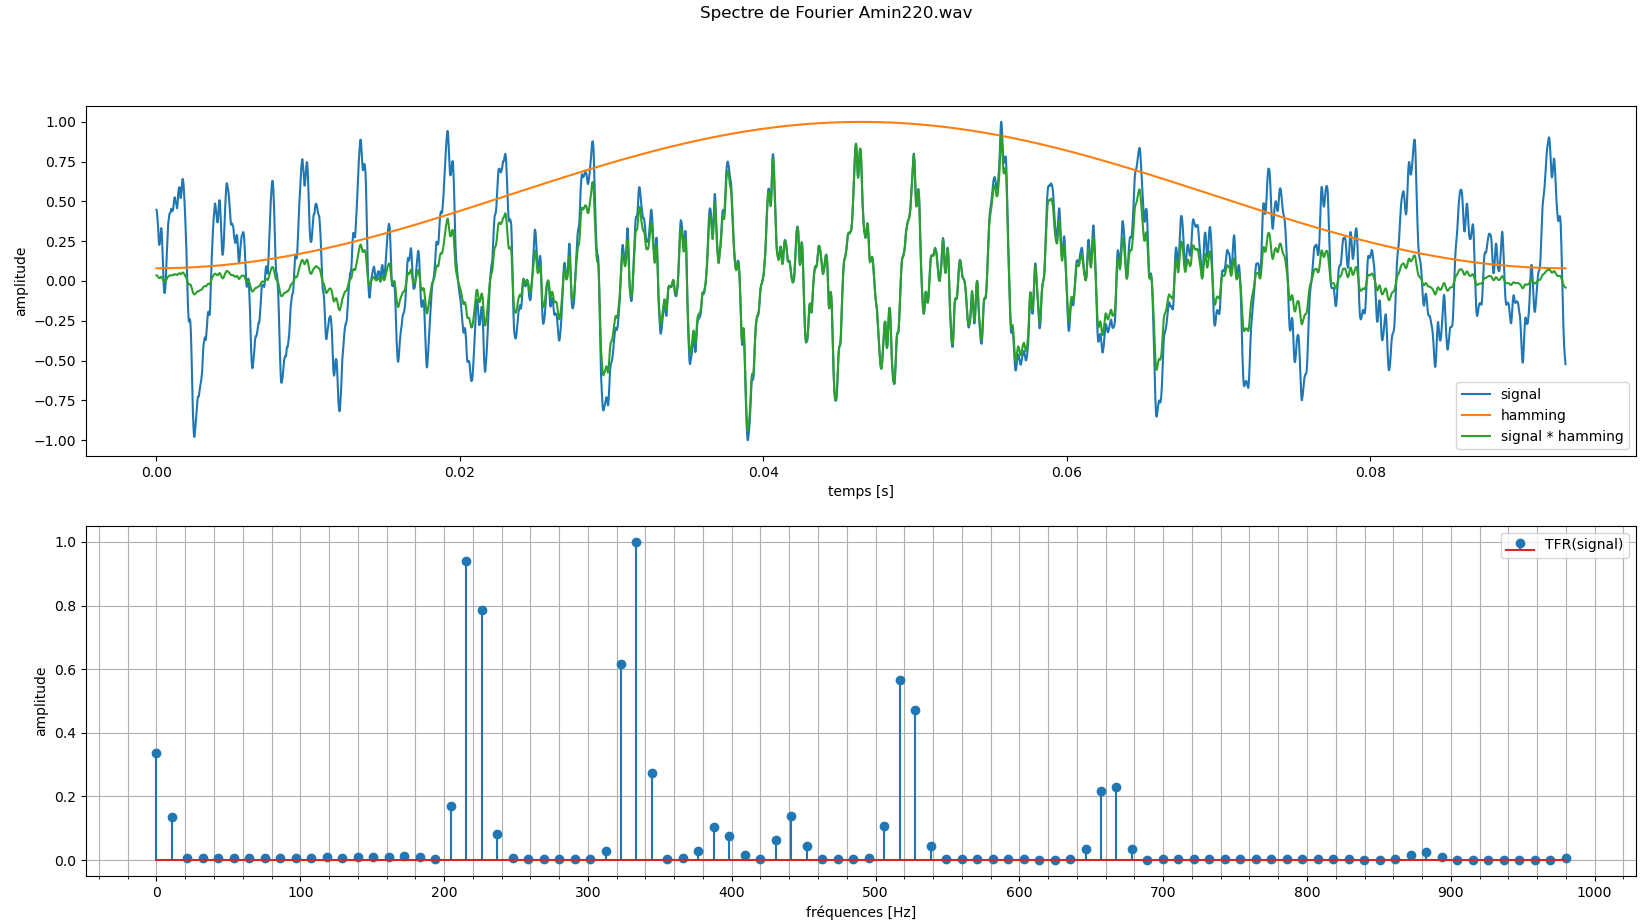
\includegraphics[width=1\linewidth]{fft_Amin220}
	\caption[Spectre de Fourier d'un Amin à 220 Hertz]{Spectre de Fourier d'un Amin à 220[Hz]. Source : Réalisé par \textsc{Küenzi} Jean-Daniel}
	\label{fig:fft_amin220}
\end{figure}

On peut remarquer que le spectre de Fourier contient beaucoup plus de pics que le précédent, ce qui est normal étant donné que notre accord est une superposition de plusieurs notes et donc signaux différents. Mais on remarque bien que nous avons le pic de la fondamentale à \textasciitilde220[Hz] ainsi que ses multiples. Ensuite, on constate un autre pic autour de 330[Hz]. Cela correspond à la quinte E, puis le pic de la tierce C autour de 520[Hz].

On peut se demander pourquoi la tierce a une fréquence plus élevée que la quinte, alors que normalement le C devrait être autour de 260[Hz]. C'est parce que généralement à la guitare on joue la tierce une octave plus haut.

% !TeX spellcheck = fr_FR
\chapter{Chapitre 3 : Apprentissage machine}
\label{chap:3}

\section{Perceptron}
\label{sec:3.1}

Le perceptron est un algorithme d'apprentissage supervisé pour des problèmes de classification linéairement séparable (classifieur binaire). Le perceptron est la forme la plus simple de réseau de neurones possible. C'est un réseau qui a des entrées, un neurone comme couche intermédiaire et une sortie. On peut facilement le représenter sous forme de fonction qui mappe une entrée $\overrightarrow{X}$ (un vecteur de valeurs réelles) à une valeur de sortie $a$ (une valeur binaire) par un produit scalaire entre les poids $\overrightarrow{W}$ et les entrées $\overrightarrow{X}$ suivi d'une fonction d'activation.

{\Large
	\setlength{\abovedisplayskip}{-0.5cm}
	\begin{gather*}
		z = \sum_{i=0}^{N-1}{W_{i}X_{i}}
	\end{gather*}
}

\begin{figure}[H]
	\centering
	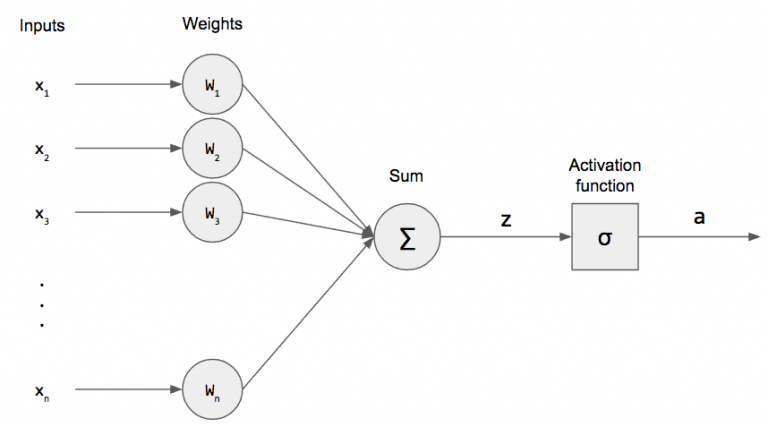
\includegraphics[width=0.7\linewidth]{perceptron}
	\caption[Perceptron]{Perceptron. Source : tiré de \textit{pythonmachinelearning.pro}, ref. URL02 / réalisé par \textsc{Deshpande} Mohit}
	\label{fig:perceptron}
\end{figure}

Les poids sont des valeurs réelles qui vont changer lorsque l’on va entrainer le perceptron. C’est-à-dire qu’on va lui faire classer une donnée dont on connait déjà la classe correcte puis une fois le classement effectué, on utilise une fonction de coût pour savoir de combien le perceptron s’est trompé. 

Par exemple l’erreur quadratique moyenne, où $Y_{i}$ représente la sortie actuelle, $\hat{Y}_{i}$ la sortie attendue et $N$ la taille.

{\Large
	\setlength{\abovedisplayskip}{-0.5cm}
	\begin{gather*}
		E[\overrightarrow{W}] = \frac{1}{N}\sum_{i=0}^{N-1}{(Y_{i} - \hat{Y}_{i})^2}
	\end{gather*}
}

Ensuite, grâce à la descente de gradient, nous pouvons trouver la valeur des poids qui minimisent la fonction de coût (l’erreur). Avec $\overrightarrow{W}$ le vecteur de poids, la mise à jour des poids $\overrightarrow{W}_t$ vers $\overrightarrow{W}_{t+1}$ peut être définie comme :

{\Large
	\setlength{\abovedisplayskip}{-0.5cm}
	\begin{gather*}
		\nabla E[\overrightarrow{W}] = [\frac{\partial E}{\partial W_{i}}] \\
		\Delta\overrightarrow{W} = -\eta\nabla E[\overrightarrow{W}] \\
		\overrightarrow{W}_{t+1} = \overrightarrow{W}_{t} + \Delta\overrightarrow{W}_{t}
	\end{gather*}
}

$\eta$ est le taux d’apprentissage, c’est un paramètre qui représente le pas que l’on va effectuer vers le minimum de la fonction de coût à chaque itération. C’est généralement un nombre assez petit, de sorte à ne pas sauter par-dessus le minimum de la fonction. Un taux d’apprentissage petit demande donc plus d’itérations pour converger et peut facilement se retrouver bloqué dans un minimum local.

Il est possible de rajouter une inertie (momentum) à la descente de gradient pour ne pas rester coincé dans un minimum local et de poursuivre la descente de gradient vers le minimum global de la fonction. Ce paramètre s'appelle généralement $\alpha$ (alpha) et il se situe entre zéro et un. Avec $\overrightarrow{W}$ le vecteur de poids et $\alpha$ l'inertie, la mise à jour des poids $\overrightarrow{W}_t$ vers $\overrightarrow{W}_{t+1}$ peut être définie comme :

{\Large
	\setlength{\abovedisplayskip}{-0.5cm}
	\begin{gather*}
		\nabla E[\overrightarrow{W}] = [\frac{\partial E}{\partial W_{i}}] \\
		\Delta\overrightarrow{W} = -\eta\nabla E[\overrightarrow{W}] \\
		\overrightarrow{W}_{t+1} = \overrightarrow{W}_{t} + \alpha\Delta\overrightarrow{W}_{t} + (1 - \alpha)\Delta\overrightarrow{W}_{t-1}
	\end{gather*}
}

\section{Fonction d'activation}
\label{sec:3.2}

Une fonction d'activation sert à définir la sortie d'un neurone par rapport à ses entrées, et donc de définir si ce neurone est activé ou non. Les fonctions d'activation sont généralement non linéaires mais il en existe plusieurs types.

{\Large
	\setlength{\abovedisplayskip}{-0.2cm}
	\begin{gather*}
		f(x) =
		\begin{cases}
			x & \: \text{si } x > 0 \\
			0 & \: \text{sinon}
		\end{cases}
	\end{gather*}
}

\begin{figure}[H]
	\centering
	
\includegraphics[width=0.5\linewidth]{relu}
	\caption[Rectified Linear Unit (ReLU)]{Rectified Linear Unit (ReLU). Source : tiré de \textit{Wikipedia}, ref. URL03}
	\label{fig:relu}
\end{figure}

\section{Perceptron Multicouche (PMC)}
\label{sec:3.3}

Un \gls{pmc} est une agrégation de couches cachées (couches entre les entrées et la sortie). Une couche est composée de perceptrons, ses entrées sont constituées de la sortie de la couche précédente (sauf pour la couche d'entrée) et sa sortie sera donc les entrées de la couche suivante.

\begin{figure}[H]
	\centering
	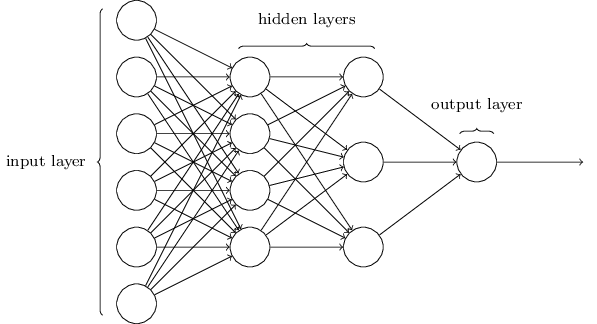
\includegraphics[width=0.7\linewidth]{pmc}
	\caption[Perceptron Multicouche (PMC)]{Perceptron Multicouche (PMC). Source : tiré de \textit{medium.com}, ref. URL04}
	\label{fig:pmc}
\end{figure}

Pour pouvoir corriger l’erreur sur les couches cachées, on utilise la technique de la rétropropagation du gradient. Le principe est d’effectuer la descente de gradient sur tous les vecteurs de poids du réseau et de propager l’erreur aux couches précédentes. Dans le cas où la fonction de coût est l’erreur quadratique et la fonction d’activation sigmoïde, la rétropropagation peut être décrite comme :

\begin{figure}[H]
	\centering
	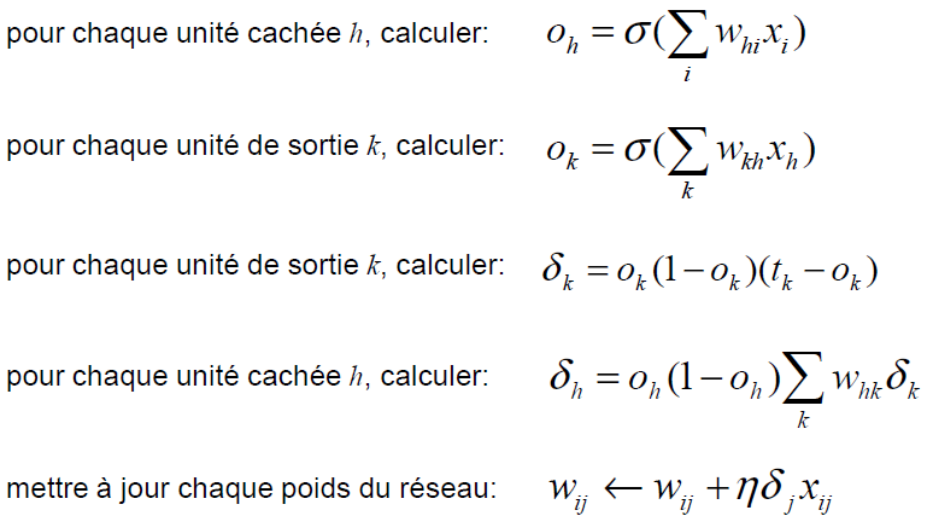
\includegraphics[width=0.7\linewidth]{backpropagation}
	\caption[Rétropropagation du gradient]{Rétropropagation du gradient. Source : tiré de \textit{l'Apprentissage Supervisé : Perceptrons Multicouche}, p. 18 / réalisé par \textsc{Bologna} Guido}
	\label{fig:retropropagation}
\end{figure}

\section{Couche de convolution}
\label{sec:3.4}

Dans le cas d'une couche de convolution, les entrées sont représentées différemment que pour le \gls{pmc}. Pour le \gls{pmc} nous avions un vecteur de valeurs réelles, la couche de convolution quant à elle prend un tenseur, c’est-à-dire un objet mathématique défini dans un espace vectoriel, et comme son nom l'indique, elle va appliquer un filtre dessus (convolution). Une couche convolutive est définie par plusieurs paramètres; il y a les canaux (filtres) qui représentent la dimension de l’espace d'entrée et de sortie de la couche, le noyau convolutif défini par sa largeur et sa hauteur (généralement symétriques) et le stride qui représente le pas de la convolution sur les dimensions.

\begin{figure}[H]
	\centering
	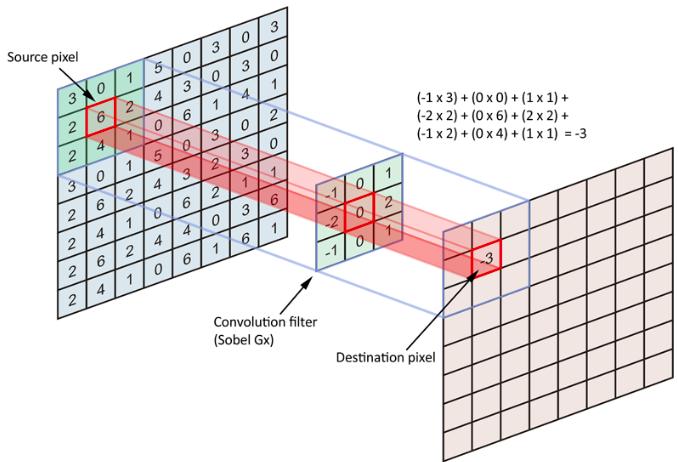
\includegraphics[width=0.7\linewidth]{convolutional_layer}
	\caption[Couche convolutive]{Couche convolutive. Source : tiré de \textit{medium.com}, ref. URL05 / réalisé par \textsc{Bui} Huy}
	\label{fig:conv_layer}
\end{figure}

\section{Couche d'agrégation}
\label{sec:3.5}

Une couche d’agrégation vient généralement après la couche de convolution et une couche de rectification (ReLU). Elle sert à résumer l’information et à diminuer le nombre de dimensions. Elle permet notamment d’éviter le surentrainement, de réduire le nombre de paramètres et de réduire la quantité de calculs nécessaires au réseau, mais surtout, elle rend le réseau invariant aux légères distorsions des données (par exemple pour la \gls{roc}, si le chiffre n’est pas situé au centre de l’image). Elle est définie par un noyau et un stride (comme pour la couche convolutive) puis par une fonction non linéaire qui va appliquer la transformation, la plus connue étant Max Pooling.

\begin{figure}[H]
	\centering
	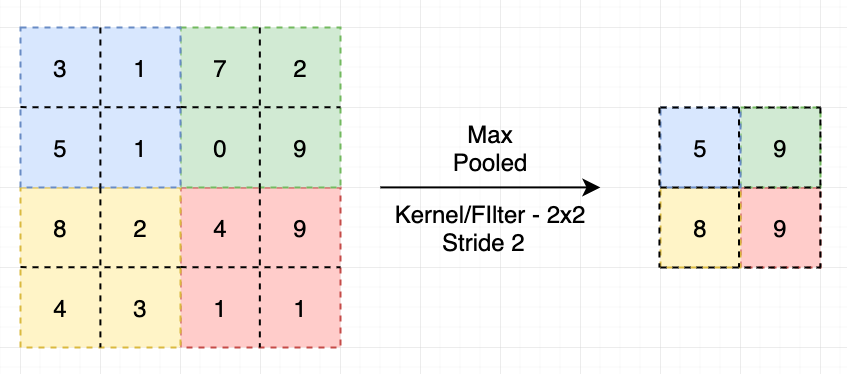
\includegraphics[width=0.7\linewidth]{pooling}
	\caption[Couche d'agrégation]{Couche d'agrégation. Source : tiré de \textit{ai.plainenglish.io}, ref. URL06 / réalisé par \textsc{Rana} Kartikeya}
	\label{fig:pooling}
\end{figure}

\section{Réseau Neuronal Convolutif (RNC)}
\label{sec:3.6}

Un \gls{rnc} est généralement utilisé dans les tâches avec des entrées fortement corrélées (la reconnaissance d'images, \gls{roc}, etc.). Dans notre cas, la détection de notes et accords de musique (séries chronologiques) présente des similarités suffisamment fortes pour qu'un \gls{rnc} semble être un choix approprié. Un \gls{rnc} possède une ou plusieurs couches convolutives entre les entrées et les couches inférieures du réseau.

\begin{figure}[H]
	\centering
	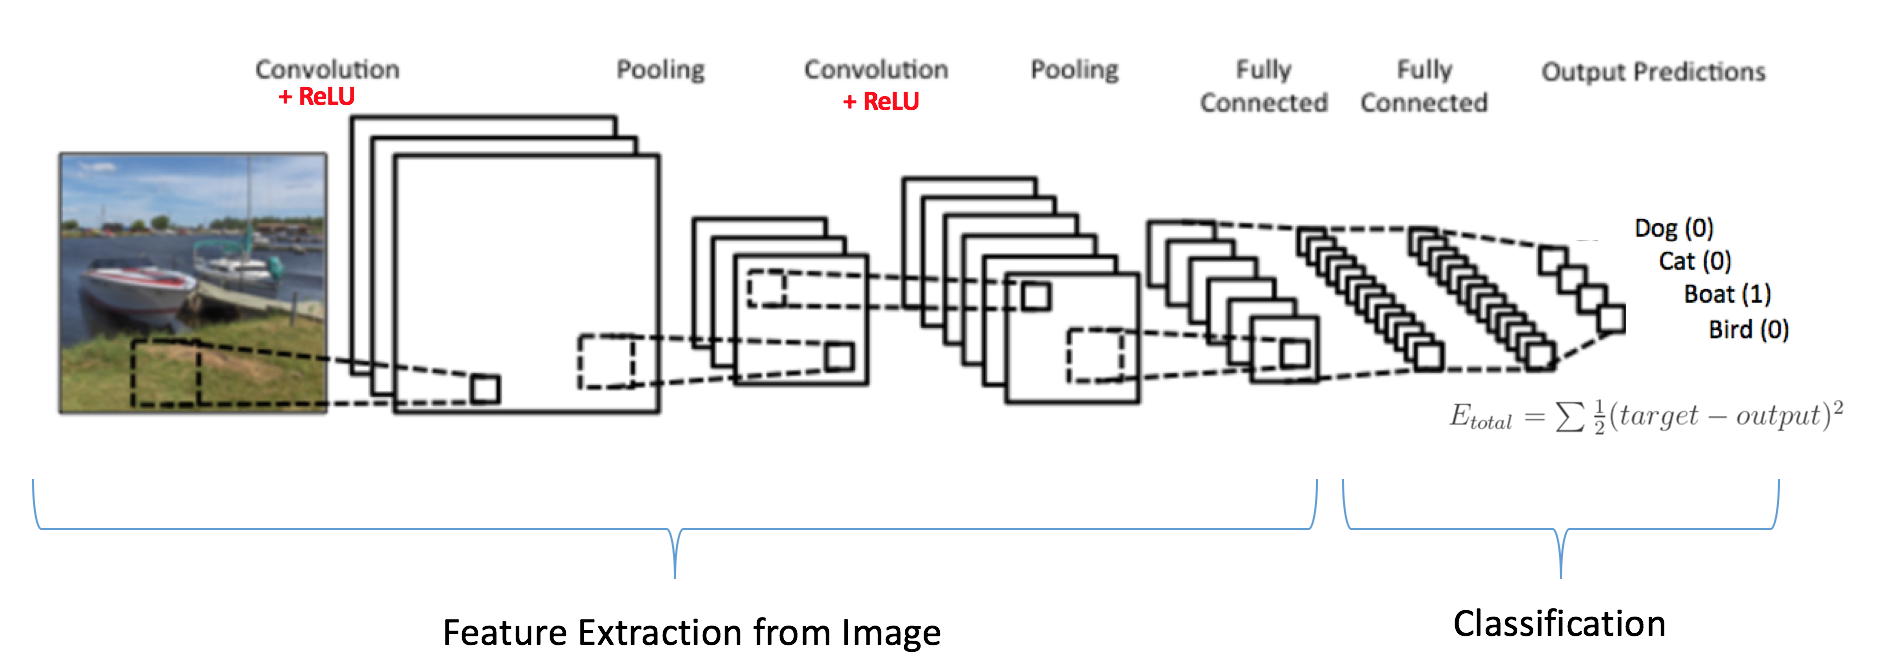
\includegraphics[width=1\linewidth]{rnc}
	\caption[Réseau Neuronal Convolutif (RNC)]{Réseau Neuronal Convolutif (RNC). Source : tiré de \textit{kdnuggets.com}, ref. URL07 / réalisé par \textsc{Ujiwal} Karn}
	\label{fig:rnc}
\end{figure}

Un \gls{rnc} peut avoir plusieurs classes en sortie (classement non-binaire); il faut donc un moyen de connaitre l’erreur pour chaque exemple. Pour cela, une fonction est appliquée à la couche de sortie, par exemple Softmax qui est une généralisation de la Sigmoïde et renvoie à un vecteur de probabilités sommant à un.

\begin{figure}[H]
	\centering
	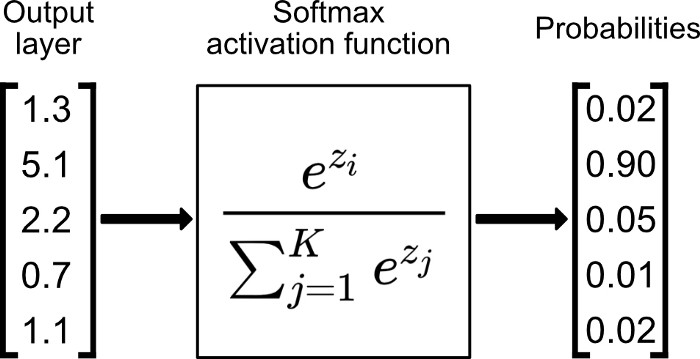
\includegraphics[width=0.5\linewidth]{softmax}
	\caption[Softmax]{Softmax. Source : tiré de \textit{towardsdatascience.com}, ref. URL08 / réalisé par \textsc{Radecic} Dario}
	\label{fig:softmax}
\end{figure}

Dans ce cas, la fonction de coût devient l’entropie croisée (somme des log-vraisemblances pour chaque classe) et elle peut se décrire comme :

\begin{figure}[H]
	\centering
	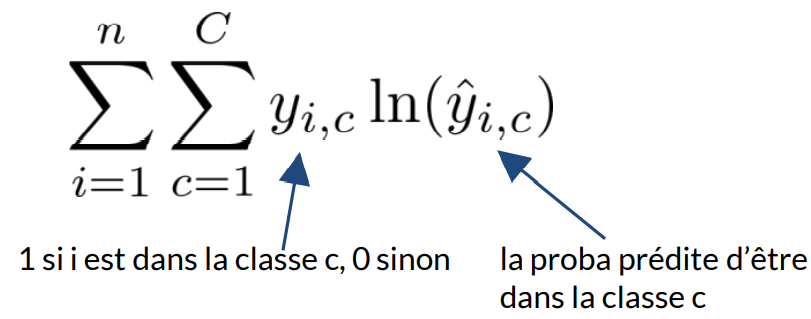
\includegraphics[width=0.5\linewidth]{cross_entropy}
	\caption[Entropie croisée]{Entropie croisée. Source : tiré de \textit{Les Réseaux Convolutifs}, p. 49 / réalisé par \textsc{Bologna} Guido}
	\label{fig:cross_entropy}
\end{figure}

\section{Long Short-Term Memory (LSTM)}
\label{sec:3.7}

Un \gls{lstm} est un type de \gls{rnr}. Une unité \gls{lstm} est généralement composée d’une cellule mémoire, d'une porte d’entrée, d'une porte de sortie et d'une porte d’oubli. Les réseaux \gls{lstm} sont de très bons réseaux lorsque l’on a des données chronologiques à traiter. Ils ont la possibilité d’oublier et de sauvegarder les données qui leur semblent utiles (extraction de caractéristiques ou \textit{features extraction} en anglais). Ils proposent aussi une solution au problème de la disparition du gradient qui est bien connu dans le domaine de l’apprentissage profond.

\begin{figure}[H]
	\centering
	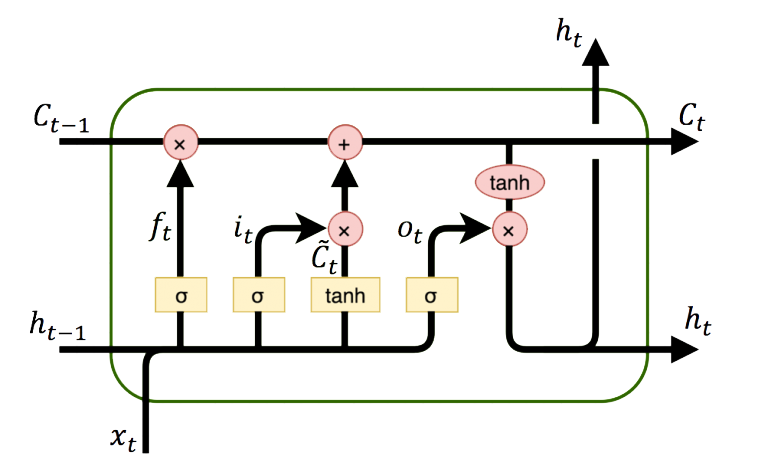
\includegraphics[width=0.7\linewidth]{lstm_cell}
	\caption[Long Short-Term Memory (LSTM)]{Long Short-Term Memory (LSTM). Source : tiré de \textit{apmonitor.com}, ref. URL09}
	\label{fig:lstm_cell}
\end{figure}

Dans les calculs suivants, nous ne tiendrons pas compte du biais. Le biais est tout simplement un neurone fictif (souvent égal à un). Il sert à décaler la fonction d’activation en y ajoutant une constante, cela aide à contrôler la valeur à laquelle la fonction d'activation s'activera.

\subsection{Porte d'oubli}

Lorsque l’on observe l’illustration \ref{fig:lstm_cell}, on remarque que la première opération effectuée est celle de la porte d’oubli. Avec $h_{t-1}$ étant l’état de la sortie à l’instant $t-1$, $X_{t}$ les entrées à l’instant $t$ et $W_{f}$ la matrice de poids, la porte d’oubli peut être décrite comme :

{\Large
	\setlength{\abovedisplayskip}{-0.5cm}
	\begin{gather*}
		f_{t} = \sigma(W_{f}[\overrightarrow{h}_{t-1}, \overrightarrow{x}_{t}])
	\end{gather*}
}

$f_{t}$ représente le vecteur d’oubli, c’est donc un vecteur de valeurs réelles entre zéro et un que l’on va multiplier avec le vecteur $C_{t-1}$, qui lui représente le vecteur de mémoire à l’instant $t-1$.

\subsection{Porte d'entrée}

La porte d’entrée quant à elle se décompose en deux parties, une première appliquant la Sigmoïde sur notre vecteur de valeurs et la deuxième qui applique Tanh.

La sortie $i_{t}$ de la sigmoïde représente un vecteur de valeurs réelles entre zéro et un. Il représente la quantité (l’importance) d’informations que l’on va garder. Avec $W_{i}$ une matrice de poids, cette partie peut être définie comme :

{\Large
	\setlength{\abovedisplayskip}{-0.5cm}
	\begin{gather*}
		i_{t} = \sigma(W_{i}[\overrightarrow{h}_{t-1}, \overrightarrow{x}_{t}])
	\end{gather*}
}

La sortie de Tanh va être un vecteur de valeurs réelles entre moins un et un. Cela correspond en quelque sorte à un vecteur de proposition, il représente les données que l’on va garder lors de la multiplication avec le vecteur $i_{t}$. Avec $W_{c}$ une matrice de poids, cette partie peut être définie comme :

{\Large
	\setlength{\abovedisplayskip}{-0.5cm}
	\begin{gather*}
		\tilde{C}_{t} = \text{Tanh}(W_{c}[\overrightarrow{h}_{t-1}, \overrightarrow{x}_{t}])
	\end{gather*}
}

\subsection{Cellule mémoire}

La cellule mémoire est toute simple, il s’agit uniquement d’un calcul où l’on multiplie le vecteur mémoire de l’état précédent ($C_{t-1}$) au vecteur d’oubli ($f_{t}$) puis on lui ajoute les nouvelles données.

{\Large
	\setlength{\abovedisplayskip}{-0.5cm}
	\begin{gather*}
		C_{t} = (C_{t-1}\times f_{t}) + (i_{t}\times\tilde{C}_{t})
	\end{gather*}
}

\subsection{Porte de sortie}

La porte de sortie se décompose également en deux étapes, une première où l’on applique la Sigmoïde sur notre vecteur de valeurs réelles, puis une deuxième où l'on multiplie la sortie de la Sigmoïde par le Tanh de notre mémoire à l’instant $t$.

Lors de la première partie, exactement comme pour la porte d’entrée, on va définir la quantité (l’importance) d’informations que l’on va garder pour notre sortie. Avec une matrice $W_{o}$, cette partie peut être décrite comme :

{\Large%
	\setlength{\abovedisplayskip}{-0.5cm}
	\begin{gather*}
		o_{t} = \sigma(W_{o}[\overrightarrow{h}_{t-1}, \overrightarrow{x}_{t}])
	\end{gather*}
}%

Pour finir, la sortie de notre unité à l’instant $t$ ($h_{t}$) est tout simplement définie comme :

{\Large%
	\setlength{\abovedisplayskip}{-0.5cm}
	\begin{gather*}
		h_{t} = o_{t}\times\text{Tanh}(C_{t})
	\end{gather*}
}%

% !TeX spellcheck = fr_FR
\chapter{Chapitre 4 : Ensemble de données}
\label{chap:4}

L'ensemble de données est séparé en deux parties; la première est destinée à l'entrainement des modèles, puis la seconde, qui est destinée à les évaluer.

Dans les deux parties, les données sont des fichiers audio mono au format wav, échantillonnés à 44.1[kHz] et encodés sur 16 bits signés. Ainsi, on respecte le théorème d'échantillonnage de Nyquist-Shanon \parencite{noauthor_theoreme_2021} et on évite le problème du repliement de spectre lors de l'analyse dans le monde des fréquences.

Nous allons tirer plusieurs extraits de ces fichiers audio qui seront nos exemples pour les différents modèles. Pour ce faire, nous allons définir une taille de fenêtre qui représentera la taille de notre exemple. Par exemple une fenêtre de 2048 échantillons, ce qui représente une résolution temporelle de \textasciitilde0.046[s] pour un signal échantillonné à 44.1[kHz].

J'ai décidé de représenter les accords à trois sons mineurs et majeurs qui se jouent sur les deux cordes les plus graves, à savoir la corde de E et de A et jusqu'à la $12^\text{ème}$ frette (case de la guitare) non incluse. Ce qui représente un total de 24 accords par corde. Les notes quant à elles sont toutes représentées.

\section{Regroupement des classes}
\label{sec:4.1}

Afin de ne pas avoir trop de classes en sortie du modèle, j'ai décidé de regrouper les classes par notes et par accords, quelle que soit l'octave dans laquelle ils se trouvent. Par exemple la classe Emaj contient le Emaj avec la basse E à \textasciitilde82[Hz] ainsi que l'accord Emaj avec la basse E à \textasciitilde164[Hz]. Même si l'accord ne se trouve pas dans la même octave, il sera classifié comme un Emaj. Pareils pour les notes, même si elles ne sont pas dans la même octave, par exemple un A à 110[Hz] et un A à 220[Hz], elles seront classifiées comme A.

J'ai pris cette décision parce que si j'avais fait une classification par octave (Amaj1 = Amaj dans la première octave, Amaj2 = Amaj dans la deuxième octave, etc.) je me serais retrouvé avec beaucoup de classes en sortie du modèle. À savoir $8 * 2$ accords (mineur, majeur) dans la première octave plus $9 * 2$ accords dans la deuxième, ce qui correspond donc à $34$ classes pour les accords mineurs et majeurs. À cela s'ajoutent les $4 * 12$ notes (chaque note est présente sur 4 octaves) pour un total de $82$ classes. En regroupant de la sorte, j'ai réduit le nombre de classes à $36$.

\section{Matériel utilisé}
\label{sec:4.2}

Pour enregistrer les fichiers, j'ai utilisé une carte son usb Roland Rubix24. Cette carte son est intéressante, car elle est entièrement blindée, ce qui réduit les interférences qui pourront se propager dans le signal et produit un bruit extrêmement faible de l'entrée à la sortie du signal. Elle m'a donc permis d'enregistrer des sons clairs et détaillés avec une excellente qualité sonore. Il est important pour le bon entrainement des modèles que l'ensemble de données soit le plus parfait et représentatif du problème que l'on veut résoudre.

Avant l'utilisation de cette carte son externe, j'avais enregistré un premier ensemble de données avec la carte son interne de mon ordinateur. Mais les signaux enregistrés à l'aide de cette carte son étaient fortement bruités, un bruit de souffle constant y était présent. On appelle ce phénomène "Bruit Blanc". J'ai constaté une nette amélioration de la précision des différents modèles après avoir enregistré le nouvel ensemble de données en utilisant la carte son externe (carte son spécialisée).

\section{Enregistrement des accords à trois sons}
\label{sec:4.3}

Dans cette partie, nous allons détailler la structure des fichiers audio qui représentent les différents accords à trois sons. Par structure, j'entends l'organisation des accords dans les fichiers et les différentes attaques que j'ai effectuées afin d'avoir un ensemble de données le plus représentatif de la réalité. Un fichier audio contiendra uniquement l'accord qui le concerne (par exemple Amaj1.wav contient uniquement Amaj).

\subsection{Ensemble de données d'entrainement}
\label{sec:4.4}

Le fichier va contenir huit fois le même accord, mais jouer avec des attaques et des manières différentes. Les deux premières fois, je vais jouer l'accord en pinçant les cordes avec les doigts, cela va me permettre de générer une attaque plutôt douce et longue dans la durée. Ensuite, les deux accords suivants sont joués en grattant les cordes avec la main, cela va produire une attaque légèrement plus brute et plus courte. Ensuite, deux accords sont joués avec le plectre (médiator) en grattant les cordes d'une manière sèche. Cela va produire une attaque très forte et très courte. Puis les deux derniers accords sont joués au plectre en arpège legato (toutes les notes de l'accord à la suite). Cette technique va décomposer l'accord en désynchronisant les différentes notes et donc signaux qui le composent.

\subsection{Ensemble de données de validation}
\label{sec:4.5}

Le fichier va contenir quatre fois le même accord. La première fois, je vais jouer l'accord en pinçant les cordes avec les doigts. Ensuite, le deuxième accord est joué en grattant les cordes avec la main. Le troisième accord est joué avec le plectre en grattant les cordes de manière sèche. Puis le quatrième accord est joué au plectre en arpège.

\section{Enregistrement des notes}
\label{sec:4.6}

Dans cette partie, nous allons détailler la structure des fichiers audio qui représentent les différentes notes. Un fichier audio contiendra la note qui le concerne dans toutes ses octaves.

\subsection{Ensemble de données d'entrainement}

La note est jouée quatre fois dans ces différentes octaves et positions sur la guitare (pour un total de 24 fois), par exemple la corde à vide d'un A qui correspond à 110[Hz] et le A sur la corde de E qui correspond aussi à 110[Hz]. Deux fois où je vais la jouer avec le doigt, produisant ainsi une attaque douce et longue. Puis, deux fois où elle sera jouée au plectre, produisant ainsi une attaque brute et courte. 

\subsection{Ensemble de données de validation}

La note est jouée deux fois dans ces différentes octaves et positions sur la guitare (pour un total de 12 fois). Une fois où je vais la jouer avec le doigt et une fois où elle sera jouée au plectre. Puis, en passant sur la corde suivante, j'alterne l'ordre donc je joue d'abord avec le plectre puis avec le doigt.

\section{Chargement de l'ensemble de données (prétraitement)}
\label{sec:4.7}

Dans cette partie, nous allons détailler les différentes techniques que j'utilise lors du chargement de mon ensemble de données ainsi que de son prétraitement. Le prétraitement des données est une étape essentielle de l'apprentissage profond, c'est dans cette partie que nous allons nettoyer et sélectionner à partir des données brutes, les données qui vont servir à entrainer les différents modèles.

\subsection{Calcul du coefficient du bruit}

Lors du chargement d'un fichier audio, il nous faut savoir quand il y a un silence et quand il n'y en a pas. En effet, nous n'aimerions pas que le réseau apprenne du silence, cela fausserait énormément les résultats. Pour ce faire, nous allons donc calculer la valeur du bruit (silence) multiplié par un coefficient de poids. Nous allons donc récupérer notre premier exemple qui se trouve au début du fichier audio puis calculer sa valeur pour avoir une référence.

Avec un signal discret $y$, un nombre d'échantillons $N$ et un coefficient de poids $W$, la valeur du bruit peut être définie comme :

{\Large
	\setlength{\abovedisplayskip}{-0.5cm}
	\begin{align*}
		P_{bruit} = \frac{W}{N}\sum_{n=0}^{N-1}{\lvert y[n]\rvert}
	\end{align*}
}

Ensuite pour chaque exemple, nous allons appliquer le même calcul sans le coefficient de poids et comparer le résultat à celui du bruit. Si la valeur est supérieure, cela veut dire qu'il ne s’agit pas d'un silence et que l'exemple est valide. Si la valeur est inférieure ou égale, il s'agit d'un silence et l'exemple n'est pas valide.

{\Large
	\setlength{\abovedisplayskip}{-0.5cm}
	\begin{align*}
		P_{exemple} = \frac{1}{N}\sum_{n=0}^{N-1}{\lvert y[n]\rvert}
	\end{align*}
}

\subsection{Chevauchement de signal}

Lorsque nous nous déplaçons dans le fichier audio (sur l'axe x) afin de récupérer nos exemples, nous allons appliquer la méthode du chevauchement de signal.

Cela consiste à définir une taille de saut qui va représenter le pas de déplacement sur l'axe x du signal. Généralement, cette taille de saut est deux ou quatre fois plus petite que la taille de la fenêtre. En effectuant un saut plus petit que la taille de la fenêtre, une partie de l'ancien exemple va se retrouver dans le nouveau.

\begin{figure}[H]
	\centering
	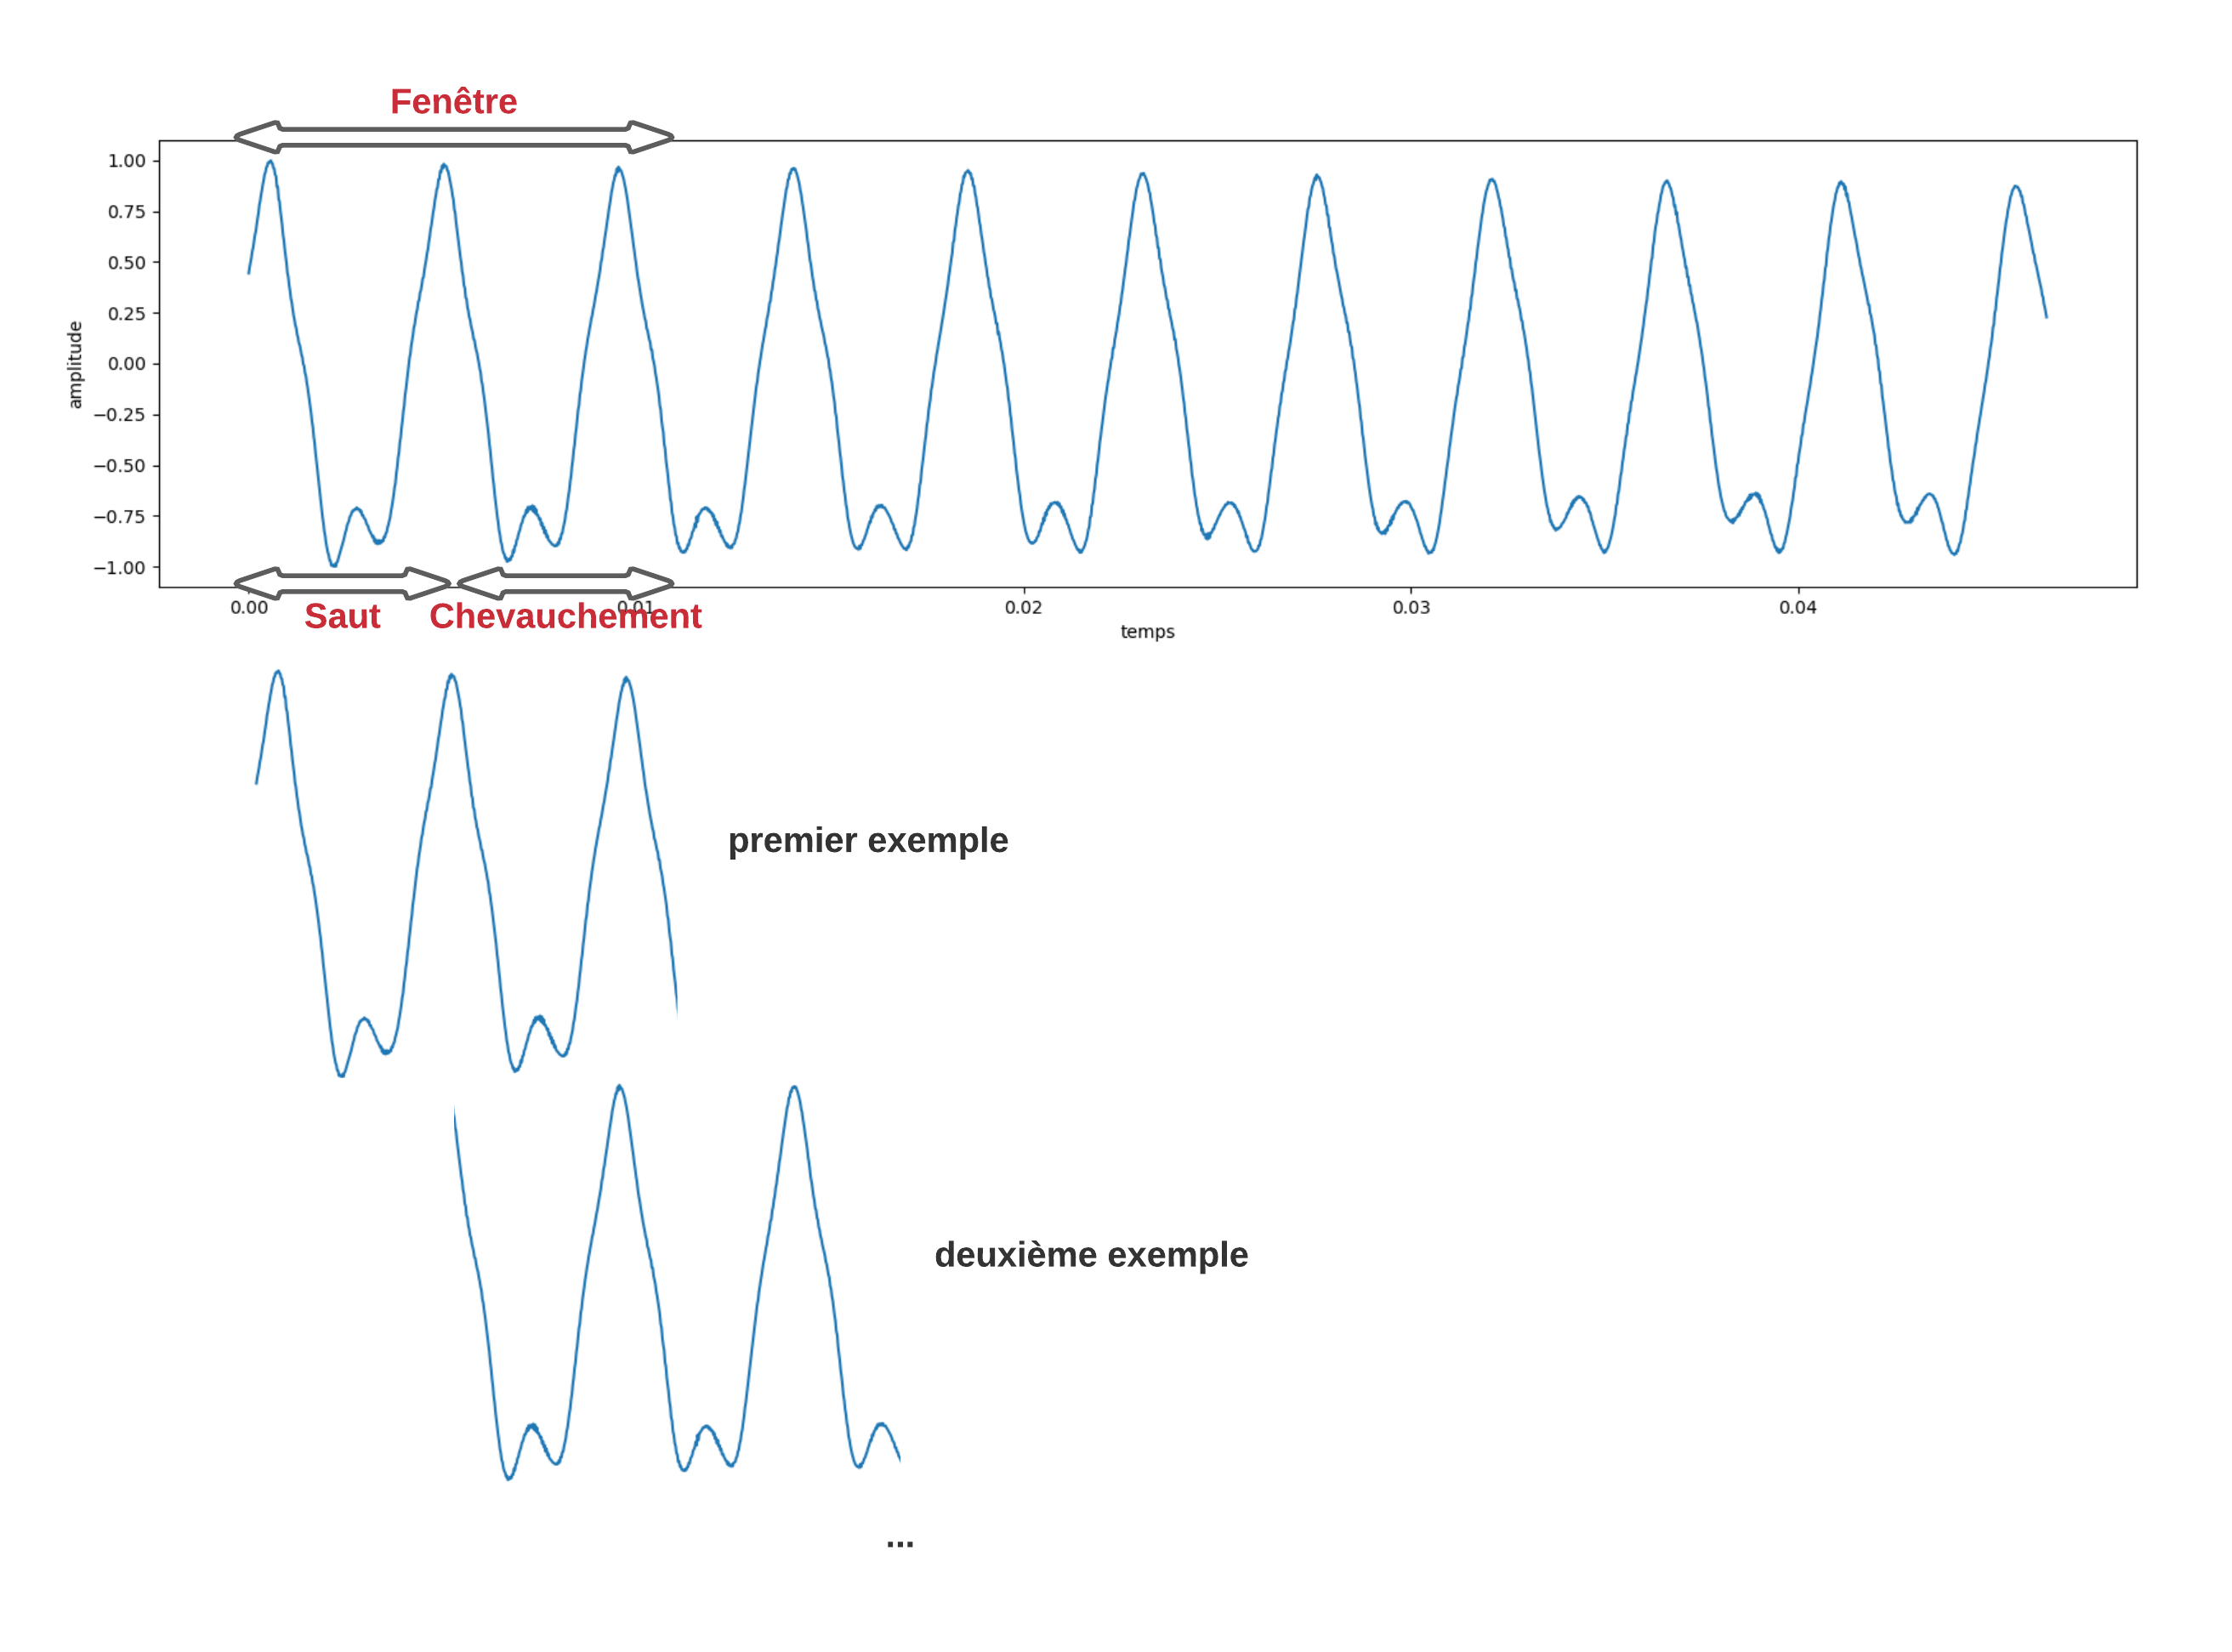
\includegraphics[width=1\linewidth]{signal_overlap}
	\caption[Chevauchement du signal]{Chevauchement du signal. Source : Réalisé par \textsc{Küenzi} Jean-Daniel. A partir de \textit{mathworks}, ref. URL10}
	\label{fig:signal_overlap}
\end{figure}

C'est une convention connue dans les analyses et traitements de série chronologique. Cela permet d'augmenter le nombre d'exemples et aussi de rendre le passage d'un exemple à un suivant beaucoup plus lisse sur l'axe x. Cela va contribuer à renforcer les modèles sur les changements de phase dans les signaux.

\subsection{Saut de l'attaque}

Finalement comme notre but est une utilisation en temps réel, l'attaque ne pose pas réellement de problème lors de la prédiction. Une attaque dure rarement plus que \textasciitilde0.02[s], donc lors de la prédiction en temps réel, elle sera à peine perceptive. En revanche elle va poser problème lors de l'entrainement du réseau. Comme elle contient beaucoup d'informations (bruit), si on essaye d'apprendre à classer l'attaque, cela va empêcher le réseau de converger correctement. Il est donc nécessaire de ne pas ajouter l'attaque dans nos exemples.

Pour ce faire, j'ai tout simplement décidé que le premier exemple valide de chaque signal était l'attaque et qu'il fallait l'ignorer. Ensuite pour ne pas retomber sur l'attaque lors du deuxième exemple, on se déplace directement sur l'axe x en utilisant la taille de la fenêtre et non la taille de saut.

\subsection{Taille de l'ensemble de données prétraité}

Le tableau ci-dessous, représente la taille de mon ensemble de données une fois qu'il est prétraité avec différentes tailles de fenêtres et donc de sauts. Une fois prétraité, l'ensemble de données sera réparti en lots (\textit{batches} en anglais) de 4'000 exemples.

\begin{table}[H]
	\centering{
		\begin{tabular}{c c l c }
			\hline
			\textbf{Nombre d'échantillons} & \textbf{Taille de saut} & \textbf{Données} & \textbf{Nombre d'exemples} \\
			\hline
			\multirow{2}{*}{1024} & \multirow{2}{*}{256} & Entrainement & 412'099 \\
			& & Validation & 254'564 \\
			\hline
			\multirow{2}{*}{2048} & \multirow{2}{*}{512} & Entrainement & 205'566 \\
			& & Validation & 127'019 \\
			\hline
			\multirow{2}{*}{3072} & \multirow{2}{*}{768} & Entrainement & 136'738 \\
			& & Validation & 84'516 \\
			\hline
			\multirow{2}{*}{4096} & \multirow{2}{*}{1024} & Entrainement & 102'347 \\
			& & Validation & 63'295 \\
			\hline
		\end{tabular}
		\caption[Taille de l'ensemble de données pour différentes tailles de fenêtres et de sauts]{Taille de l'ensemble de données pour différentes tailles de fenêtres et de sauts. Source : Réalisé par \textsc{Küenzi} Jean-Daniel}
		\label{tab:dataset}
	}
\end{table}
% !TeX spellcheck = fr_FR
\chapter{Chapitre 5 : Conception}
\label{chap:5}

\section{Architecture LSTMB avec TFR}
\label{sec:5.1}

\begin{figure}[H]
	\centering
	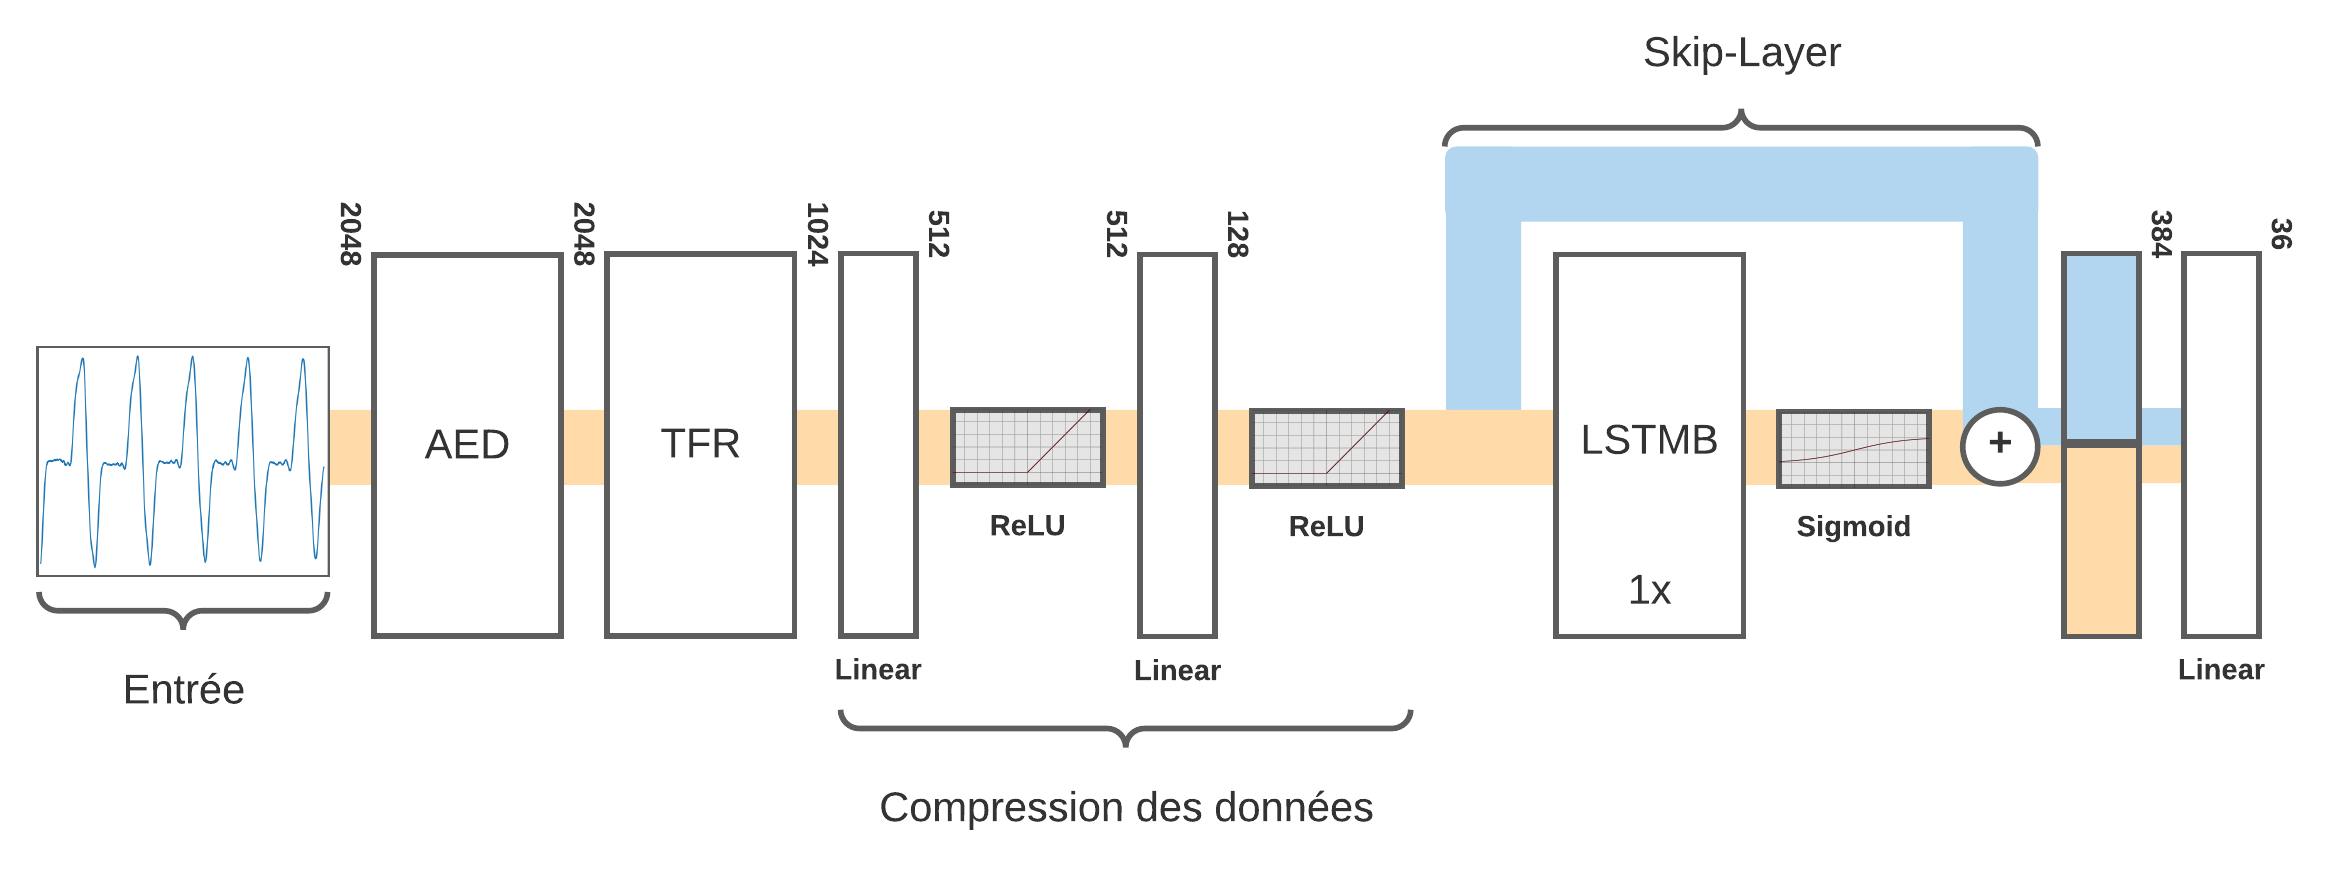
\includegraphics[width=1\linewidth]{lstmb_fft}
	\caption[Architecture LSTMB avec TFR]{Architecture LSTMB avec TFR. Source : Réalisé par \textsc{Küenzi} Jean-Daniel}
	\label{fig:lstmb_fft}
\end{figure}

Dans cette thèse je vais uniquement présenter les architectures avec la \gls{tfr} car ce sont celles qui ont fourni les meilleurs résultats. Les architectures que j'ai utilisées avec les données discrètes se trouvent en annexe. Il s'agit tout simplement de la même architecture sans la \gls{tfr} et avec des couches de normalisation par lots (voir \autoref{sec:5.5}) en plus.

\section{Auto-encodeur débruiteur (AED)}
\label{sec:5.2}

J'ai appris la connaissance de l'\gls{aed} en lisant le document "Autoencoders" \parencite{bank_autoencoders_2021}. Je voulais trouver un moyen de retirer le bruit de mes données de manière rapide (nécessaire pour l'utilisation en temps réel) et sans avoir à passer par des filtres à convolution. Il était important de pouvoir réduire le bruit dans un signal dans le cas où nous n'utilisons pas du matériel spécialisé dans le traitement audio. De plus, je me suis dit que cela pourrait aider à réduire les différents effets, comme le gain ou la distorsion, que nous pouvons ajouter sur le signal. Cette réduction pourra donc aider le modèle à prédire plus facilement l'accord ou la note. En temps réel et dans le monde de l'audio, la latence que l'on est prêt à accepter est en dessous de cinq millisecondes pour le traitement du son (les calculs). D'où la nécessité d'avoir une méthode rapide et simple.

Le but d'un \gls{aed} est de reconstruire les données originales non bruitées à partir de données bruitées. Pour ce faire, on va volontairement bruiter les données qui vont servir d'exemples lors de l'entrainement en rajoutant du bruit blanc gaussien $X\rightarrow\tilde{X}$ et en entrainant l'\gls{aed} à reconstruire les données non bruitées en calculant la perte $L(\tilde{X}, X)$.

Il existe plusieurs types d'auto-encodeurs et différentes architectures, mais j'ai décidé d'opter pour une architecture profonde en bottle-neck afin de ne pas perdre trop de temps en traversant le réseau. Comme nous voulons prédire en temps réel, il doit y avoir le moins de temps possible passé à traverser le réseau.

Lorsque le signal va passer dans l'\gls{aed}, il va être séparé un huit vecteurs de taille 256, puis il sera reconstruit en un vecteur de taille 2048 à la fin, juste avant d'être normalisé à nouveau. On effectue une séparation, car l'architecture dense utilisée est plus efficace pour réduire le bruit sur des petites tailles de vecteurs que sur des grandes.

\subsection{Architecture}

\begin{figure}[H]
	\centering
	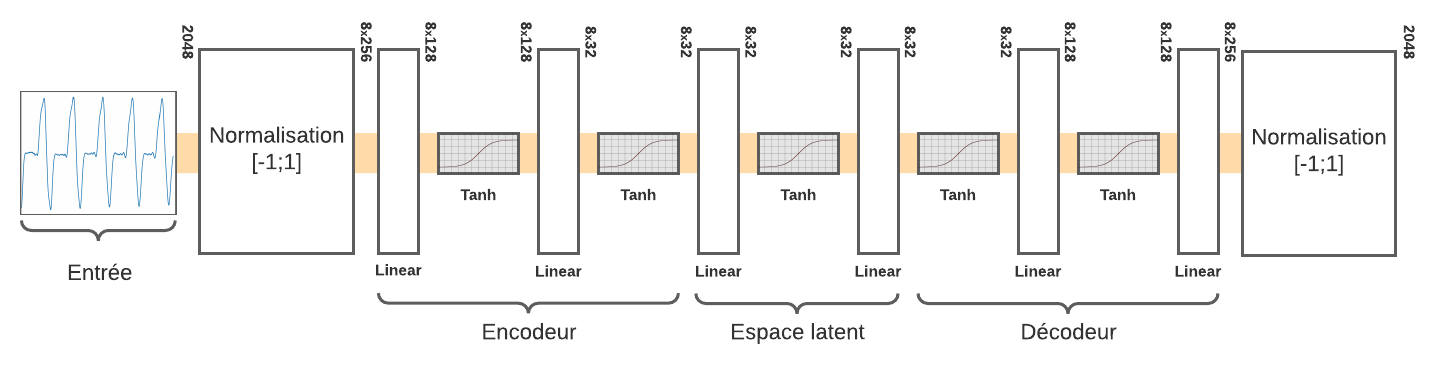
\includegraphics[width=1\linewidth]{aed}
	\caption[Architecture AED]{Architecture AED. Source : Réalisé par \textsc{Küenzi} Jean-Daniel}
	\label{fig:aed}
\end{figure}

\subsection{Bruit blanc gaussien}

Le bruit blanc gaussien est un type de bruit qui est utilisé pour corrompre des données et qui est largement utilisé dans le monde des \gls{aed}. Il est très intéressant, car sa puissance est uniforme sur toute la largeur de bande de fréquences et il suit une loi de distribution normale (gaussienne). Le bruit qui a été ajouté a une moyenne de zéro et un écart type de zéro virgule trois. Dans le monde des signaux, il peut être comparable à un bruit de souffle constant assez fort.

\subsection{Normalisation}

Lorsque le signal va passer à travers l'\gls{aed}, il va être normalisé à son entrée puis à sa sortie. La normalisation des données est d'une importance capitale pour le réseau, cela va lui permettre de ne pas apprendre les amplitudes des signaux et va lui permettre de se concentrer sur d'autres caractéristiques. Aussi, la normalisation va aidée l'\gls{aed} à se faire sa propre représentation des données dans son espace latent et à converger plus rapidement.

La normalisation effectuée est une Min-Max avec une plage entre moins un et un. Son avantage est qu'elle est rapide à faire et elle va conserver le rapport entre les différentes amplitudes du signal (la forme du signal reste inchangée). Avec un signal discret $Y$ et le signal discret normalisé $Y'$, la normalisation appliquée peut être définie comme :

{\Large
	\setlength{\abovedisplayskip}{-0.5cm}
	\begin{align*}
		Y' = 2\frac{Y-\text{min}(Y)}{\text{max}(Y)-\text{min}(Y)}-1
	\end{align*}
}

\subsection{Espace latent}

L'espace latent est une représentation compressée des données que le réseau va apprendre de lui-même. Lors de l'entrainement, il va apprendre à extraire les caractéristiques qui lui semble les plus pertinentes et va ensuite les utiliser afin de reconstruire les données non bruitées.

\subsection{Perte de reconstruction}

Pour un auto-encodeur, on parle de perte de reconstruction pour signifier la différence entre les données attendues et les données reconstruites. La fonction que j'ai utilisée pour calculer ma perte de reconstruction est l'erreur quadratique moyenne. Avec $Y_{i}$ la sortie actuelle, $\hat{Y}_{i}$ la sortie attendue et $N$ la taille. L'erreur quadratique moyenne peut être définie comme :

{\Large
	\setlength{\abovedisplayskip}{-0.5cm}
	\begin{align*}
		E[\overrightarrow{W}] = \frac{1}{N}\sum_{i=0}^{N-1}{(Y_{i} - \hat{Y}_{i})^2}
	\end{align*}
}

\section{Transformée de Fourier rapide (TFR)}
\label{sec:5.3}

Une fois que le signal est passé par l'\gls{aed}, on va effectuer une \gls{tfr} afin de récupérer son spectre. Mais avant de faire la \gls{tfr}, nous allons multiplier le signal par une fenêtre de Hamming afin de réduire la fuite spectrale et de faciliter ainsi l'apprentissage au réseau.

\subsection{Composante du spectre continu}

Comme vu dans la \autoref{sec:2.8}, nous nous intéressons uniquement à la partie du spectre continu. Donc lorsque que nous effectuons une \gls{tfr} avec une fenêtre de taille $N$ nous allons uniquement prendre en compte les $N/2$ premiers coefficients de Fourier. Cette réduction de moitié permet au réseau d'être plus précis sur ses prédictions et plus rapide. Comme la \gls{tfr} retourne des nombres complexes, c'est le module de ses nombres que l'on va passer au réseau (voir \autoref{sec:2.8}).

\subsection{Normalisation}

Une fois la \gls{tfr} faite, nous allons normaliser les données afin que la valeur des amplitudes ne soit pas un facteur que le réseau doivent apprendre. Finalement, tout ce qui nous intéresse c'est uniquement de connaitre les fréquences et non leurs amplitudes. On va donc pouvoir normaliser le spectre obtenu afin de faciliter au réseau l'apprentissage et la prédiction.

La normalisation effectuée est une Min-Max avec une plage entre zéros et un. Son avantage est qu'elle est rapide à faire et elle va conserver le rapport entre les différentes amplitudes du spectre. Avec un signal discret $Y$ et le signal discret normalisé $Y'$, la normalisation appliquée peut être définie comme :

{\Large
	\setlength{\abovedisplayskip}{-0.5cm}
	\begin{align*}
		Y' = \frac{Y-\text{min}(Y)}{\text{max}(Y)-\text{min}(Y)}
	\end{align*}
}

\section{Compression des données}
\label{sec:5.4}

Comme pour l'\gls{aed}, cette couche va permettre au réseau de se faire sa propre représentation des données qu'il reçoit de la \gls{tfr}. Lors de l'entrainement, il va apprendre à extraire les caractéristiques qui lui semblent importantes. Cette couche est ajoutée afin de permettre aux données de traverser plus rapidement le réseau sans perdre pour autant la précision.

\section{Normalisation par lots}
\label{sec:5.5}

La normalisation par lots ou (\textit{Batch Normalization} en anglais) est une technique décrite dans le document "Batch Normalization: Accelerating Deep Network [...]" \parencite{ioffe_batch_2015}. Le principe est de rajouter des couches qui vont aider à mieux coordonner la mise à jour des poids lors de la rétropropagation du gradient. Elle rend notamment le réseau moins dépendant du paramétrage initial comme le taux d'apprentissage et la génération aléatoire des poids. Elle permet aussi dans certains cas de ne pas avoir besoin de recourir à des couches de dropout.

En apprentissage profond, lors de la rétropropagation du gradient, on corrige les poids d'une couche à partir d'une estimation de l'erreur en supposant que les poids des couches précédentes sont fixes. Mais finalement comme nous mettons à jour toutes les couches du réseau simultanément cette supposition est fausse. Cela nous oblige à faire attention aux paramètres d'initialisations du réseau et ralentit l'entrainement en nous contraignant à utiliser un petit taux d'apprentissage. Dans le document \parencite{ioffe_batch_2015}, ce problème est nommé "Changement de Covariable Interne" (\textit{Internal Covariate Shift} en anglais).

La normalisation par lots va nous aider à régler ce problème en normalisant les entrées des couches par mini-lots (\textit{mini-batchs} en anglais) pour avoir une moyenne de zéro et un écart type de un. Cette normalisation permet au réseau durant la rétropropagation du gradient de mieux régulariser l'erreur et de rendre la mise à jour des poids moins propice à varier de manière drastique.

Cette problématique de réduction du changement de covariable interne reste encore discutée. D'autres études comme "How Does Batch Normalization Help Optimization?" \parencite{santurkar_how_2019} estiment que la normalisation par lots aide l'entrainement du réseau en rendant la descente de gradient plus lisse et simplifie donc la convergence du réseau.

Il est aussi possible de permettre à la couche de normalisation d'apprendre deux paramètres, $\beta$ et $\gamma$. Généralement cela se fait beaucoup, car normaliser les entrées des couches peut modifier la représentation de la couche. Ces deux paramètres permettent de s'assurer de pouvoir retrouver la transformation identité (la réelle représentation).

Avec $x$ les entrées, $E[x]$ l'erreur pour chaque entrée, $\text{Var}[x]$ l'écart type pour chaque entrée, $\epsilon$ une valeur ajoutée pour la stabilité numérique, $\beta$ et $\gamma$ les deux paramètres apprenables. PyTorch \parencite{noauthor_batchnorm1d_nodate} définit la normalisation par lots comme :

{\Large
	\setlength{\abovedisplayskip}{-0.5cm}
	\begin{align*}
		y = \frac{x - E[x]}{\sqrt{\text{Var}[x] + \epsilon}}\times\gamma+\beta
	\end{align*}
}

J'ai utilisé les couches de normalisation par lots lors de la prédiction avec les données discrètes (sans \gls{tfr}) car cela avait un impacte non négligeable sur la précision des modèles. Mais lors de l'utilisation avec les données de la \gls{tfr} j'ai constaté une perte de précision. Les couches de normalisation par lots sont ajoutées après les couches denses et les couches de convolution mais avant la fonction d'activation ReLU qui est non linéaire, comme précisé dans le document \parencite{ioffe_batch_2015}. Les tableaux ci-dessous représentent les différences d'entrainements de l'architecture LSTMB sans \gls{tfr} (voir \autoref{app:1}) avec et sans couches de normalisation par lots.

\begin{table}[H]
	\centering{
		\begin{tabular}{l c c}
			\hline
			\multicolumn{3}{c}{\textbf{Sans la normalisation par lots}} \\
			\multicolumn{3}{c}{epochs = 50, $\eta$ = 0.005, nombre d'entrainements = 10} \\
			\hline
			\textbf{Données} & \textbf{Précision moyenne \%} & \textbf{Ecart type \%}\\
			\hline
			Entrainement & 98.19 & 0.43 \\
			Validation & 88.36 & 0.51 \\
			\hline
		\end{tabular}
		\caption[Entrainement sur données discrètes sans la normalisation par lots]{Entrainement sur données discrètes sans la normalisation par lots. Source : Réalisé par \textsc{Küenzi} Jean-Daniel}
		\label{tab:without_batchnorm}
	}
\end{table}

\begin{table}[H]
	\centering{
		\begin{tabular}{l c c}
			\hline
			\multicolumn{3}{c}{\textbf{Avec la normalisation par lots}} \\
			\multicolumn{3}{c}{epochs = 50, $\eta$ = 0.005, nombre d'entrainements = 10} \\
			\hline
			\textbf{Données} & \textbf{Précision moyenne \%} & \textbf{Ecart type \%}\\
			\hline
			Entrainement & 99.91 & 0.02 \\
			Validation & 92.45 & 0.54 \\
			\hline
		\end{tabular}
		\caption[Entrainement sur données discrètes avec la normalisation par lots]{Entrainement sur données discrètes avec la normalisation par lots. Source : Réalisé par \textsc{Küenzi} Jean-Daniel}
		\label{tab:with_batchnorm}
	}
\end{table}

En observant les résultats, on constate bien l'efficacité de ces couches de normalisation par lots. Avec les mêmes paramètres d'initialisation, le modèle a convergé beaucoup plus rapidement et l’on a ainsi gagné un peu plus de quatre pour cent de précision moyenne sur l'ensemble de validation.

\section{Cellule LSTM Bidirectionnelle (LSTMB)}
\label{sec:5.6}

Une cellule \gls{lstmb} est en fait composé de deux cellules \gls{lstm}. Une qui va propager $h_t$ vers l'avant et une qui va le propager vers l'arrière. On peut voir sa comme recevoir les informations du passé et du futur à la fois. Une cellule LSTM classique utilise $h_{t-1}$ (passé) pour produire $h_t$. Une cellule \gls{lstmb} va à la fois utiliser $h_{t-1}$ et $h_{t+1}$ (futur) pour produire $y_t$ qui est notre sortie. En fait $y_t$ est tout simplement une concaténation (parfois accompagné d'une fonction d'activation) des sorties $h_t$ des deux cellules (voir \autoref{fig:bidirectional_lstm}). Comme on récupère la sortie des deux cellules et qu'on concatène, on à plus de données à la sortie qu'à l'entrée.

Donc dans notre cas, on peut voir qu'on a un vecteur de taille 128 à l'entrée de la cellule et on aura donc un vecteur de taille 256 à sa sortie, on a augmenté la taille de nos données par un facteur deux.

\subsection{Architecture}

\begin{figure}[H]
	\centering
	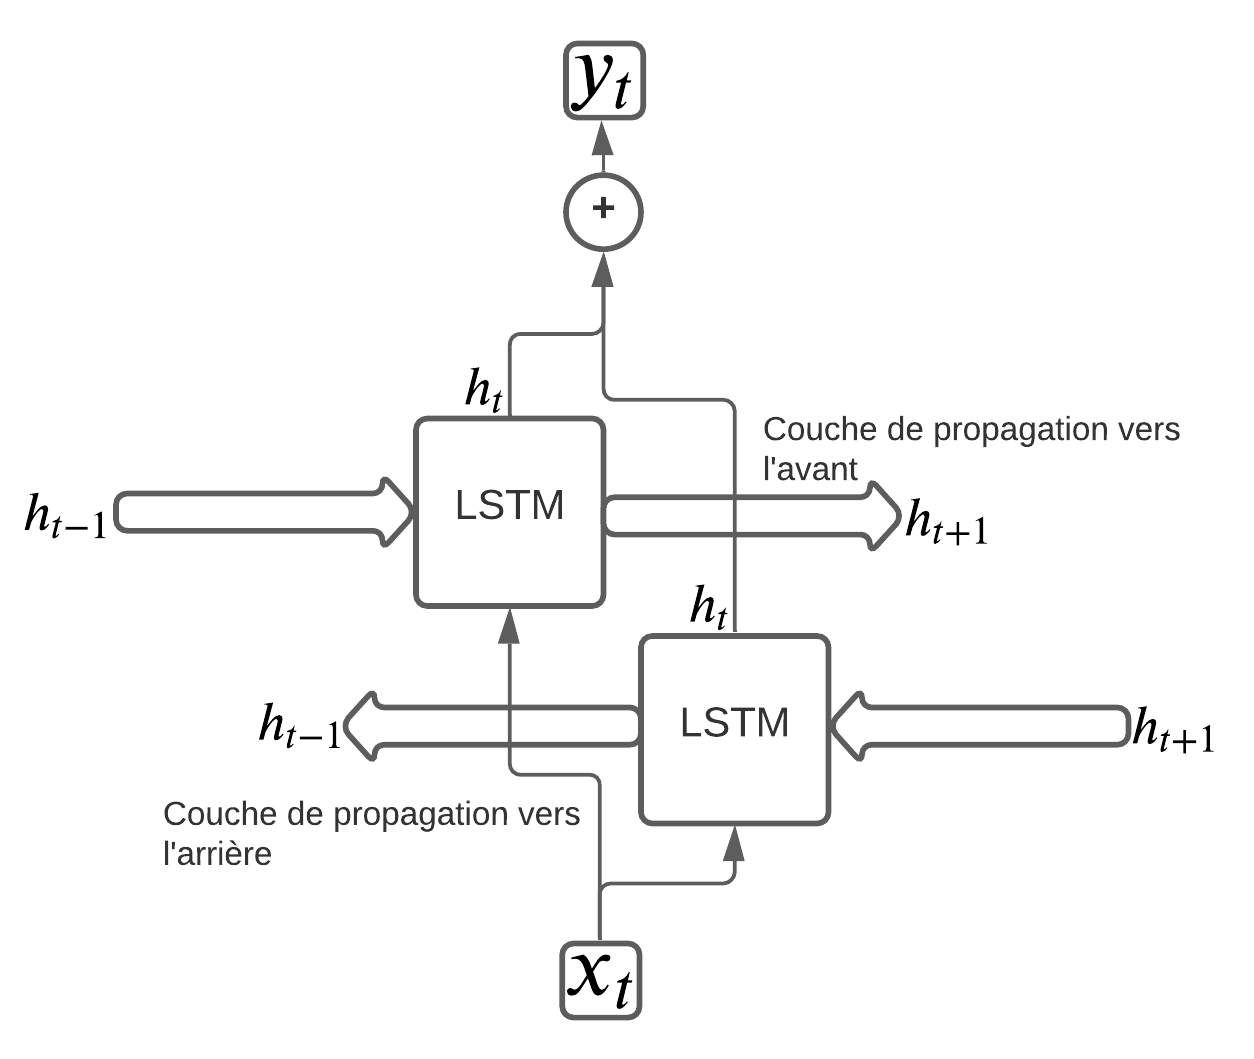
\includegraphics[width=0.7\linewidth]{bidirectional_lstm}
	\caption[Cellule LSTM Bidirectionnelle]{Cellule LSTM Bidirectionnelle. Source : Réalisé par \textsc{Küenzi} Jean-Daniel}
	\label{fig:bidirectional_lstm}
\end{figure}

\section{Skip-Layer}
\label{sec:5.7}

La Skip-Layer est en fait une technique utilisée où, comme son nom l'indique, on va éviter des couches. Comme on peut le voir sur la \autoref{fig:lstmb_fft}, une copie des données vont êtes prises avant de traverser la cellule \gls{lstmb} et vont ensuite être concaténée à sa sortie. La skip-layer va permettre aux couches suivantes d'apprendre également des données qui se trouvent avant la cellule \gls{lstmb}. Elle aide aussi pour la rétropropagation du gradient, notamment en aidant à éviter le problème du gradient de fuite. La Skip-Layer est beaucoup utilisée dans les architectures modernes.

\section{Fonction de coût}
\label{sec:5.8}

La fonction de coût que j'ai utilisé est l'entropie croisée (\textit{cross-entropy} en anglais). PyTorch \parencite{noauthor_crossentropyloss_nodate} utilise une combinaison de la fonction de perte logarithmique de vraisemblance négative (\textit{Negative Log-Likelihood Loss} en anglais) et de la fonction Logarithmique Softmax (\textit{Log-Softmax} en anglais), qui est tous simplement le logarithme de la fonction softmax. En pratique, on préfère l'utilisation de la fonction log-softmax plutôt que la fonction softmax. Elle est plus utilisée, car la fonction log-softmax aide le réseau en assurant une stabilité numérique de l'erreur. Elle ne va jamais devenir infiniment petite. Aussi, de par sa nature exponentielle elle inflige des pénalités beaucoup plus lourdes que la softmax (qui est linéaire) pour les classes incorrectes, et aide donc le réseau à converger plus vite. Pour finir, elle est optimisée pour effectuer moins de calculs que la softmax durant la descente de gradient. Avec $x$ un tenseur de valeurs réelles. PyTorch définit la log-sofmax comme :

{\Large%
	\setlength{\abovedisplayskip}{-0.5cm}
	\begin{gather*}
		\text{LogSoftmax}(x_i) = \text{log}(\frac{\text{exp}(x_i)}{\sum_{j}{\text{exp}(x_j)}})
	\end{gather*}
}%

et donc avec $x$ un tenseur de valeurs réelles qui représente la sortie du réseau et $y$ un tenseur correspondant aux classes correctes attendues, PyTorch \parencite{noauthor_crossentropyloss_nodate} définit l'entropie croisée comme

{\Large%
	\setlength{\abovedisplayskip}{-0.5cm}
	\begin{gather*}
		\text{L}(x, y) = -x_y + \text{log}(\sum_{j}{\text{exp}(x_j)})
	\end{gather*}
}%


% !TeX spellcheck = fr_FR
\chapter{Chapitre 6 : Expérimentation}
\label{chap:6}

\section{PMC}
\label{sec:6.1}

\subsection{Architecture avec TFR}

\begin{figure}[H]
	\centering
	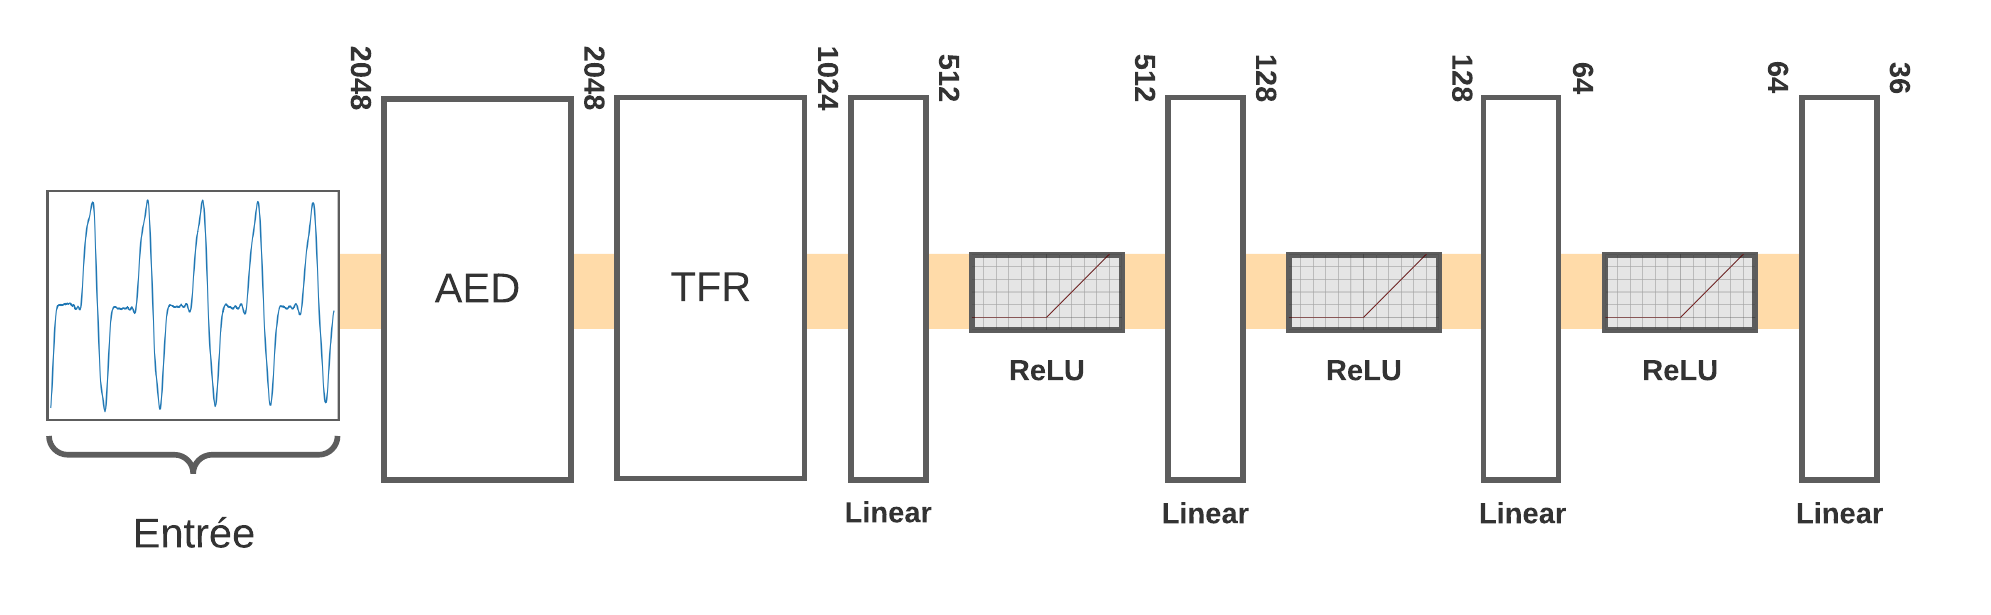
\includegraphics[width=1\linewidth]{mlp_fft}
	\caption[Architecture PMC avec TFR]{Architecture PMC avec TFR. Source : Réalisé par \textsc{Küenzi} Jean-Daniel}
	\label{fig:mlp_fft}
\end{figure}

\subsection{Matrice de confusion sur l'ensemble de validation}
\label{subsec:6.1.2}

La matrice de confusion suivante a été réalisée avec le modèle utilisant une fenêtre de 2048 échantillons.

\begin{figure}[H]
	\centering
	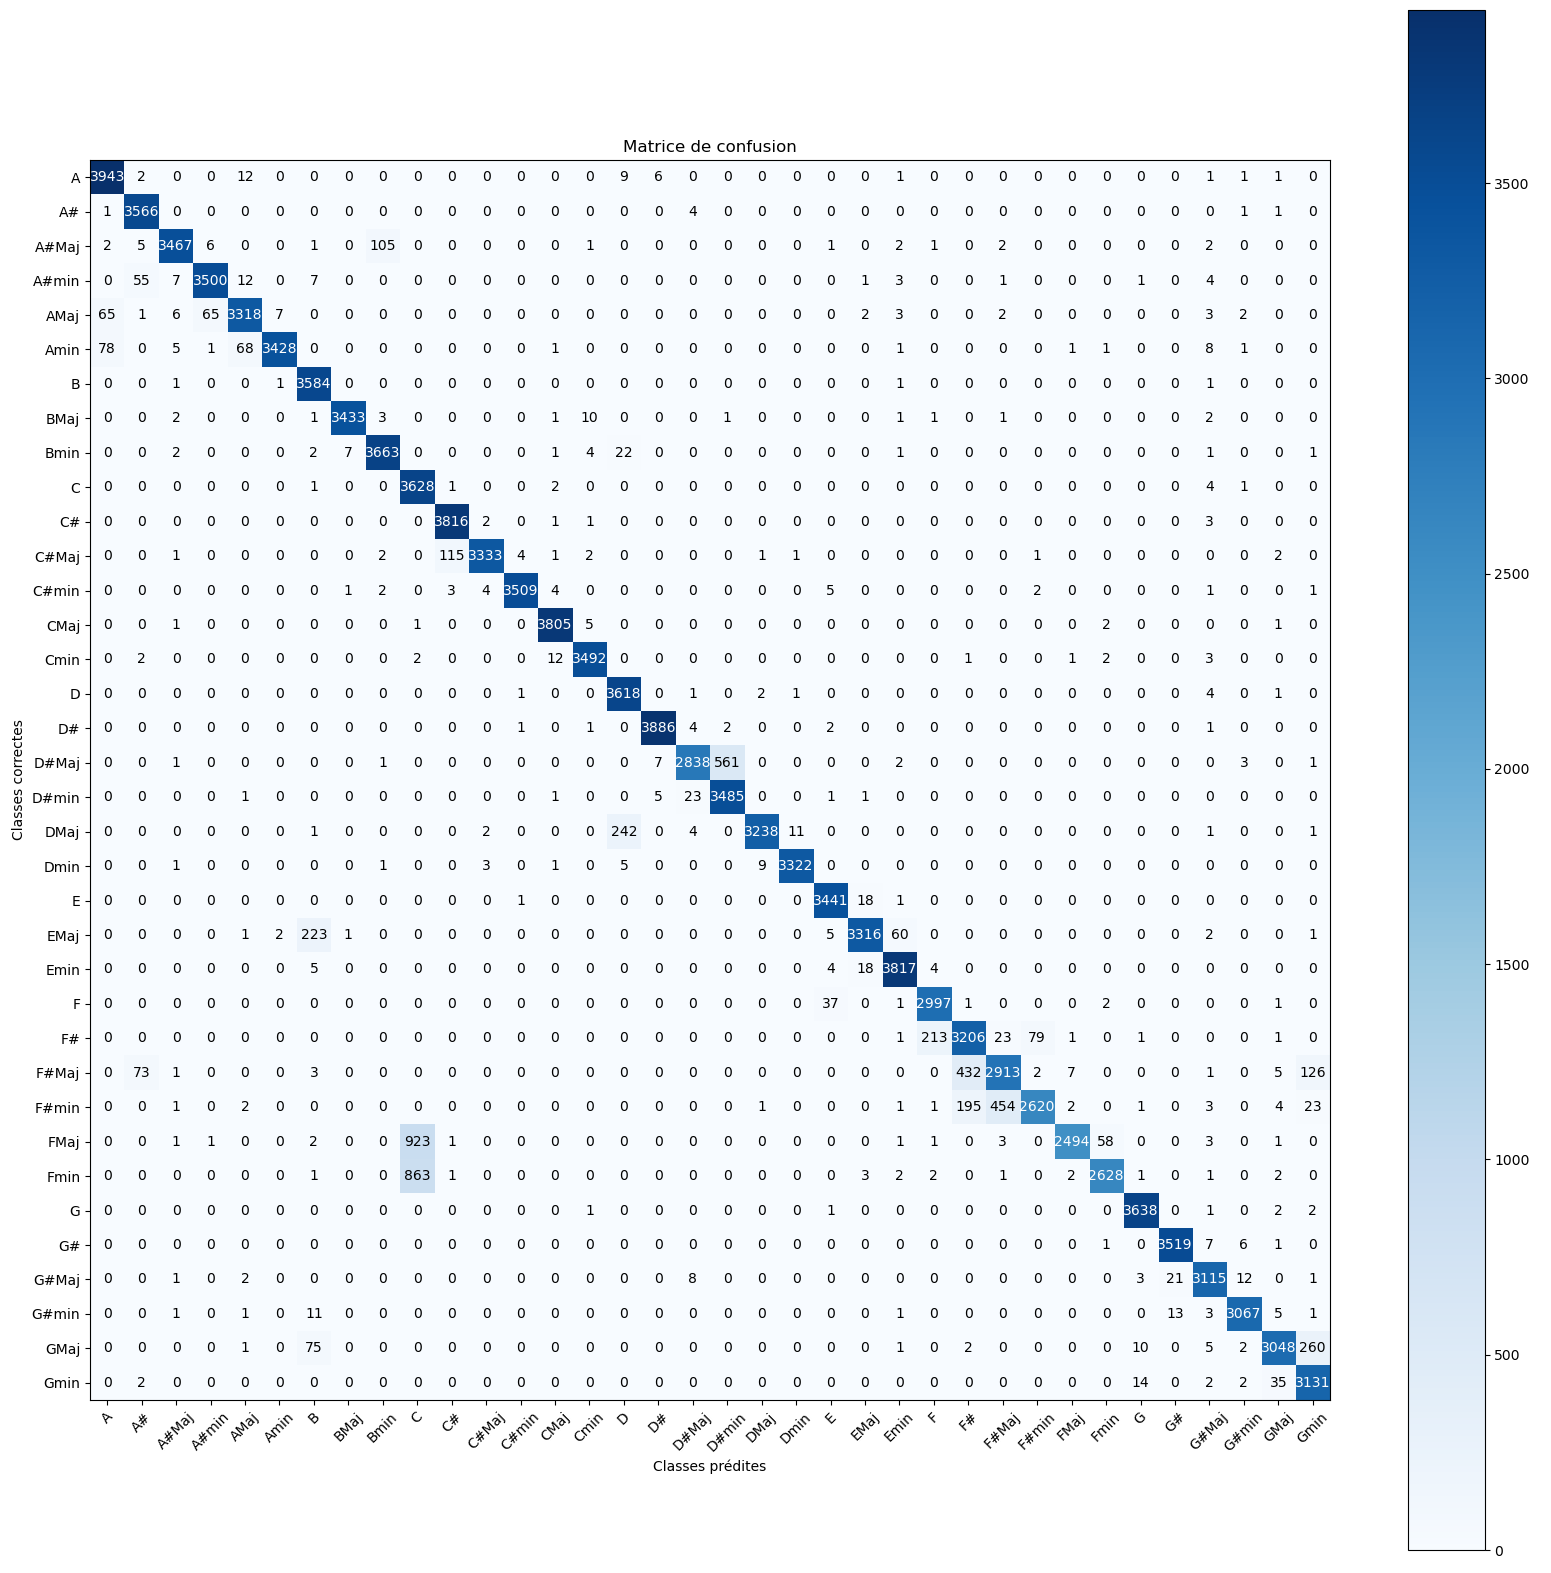
\includegraphics[width=1\linewidth]{cm_mlp_fft}
	\caption[Matrice de confusion pour l'architecture PMC avec TFR]{Matrice de confusion pour l'architecture PMC avec TFR. Source : Réalisé par \textsc{Küenzi} Jean-Daniel}
	\label{fig:cm_mlp_fft}
\end{figure}

Lorsque l'on observe cette matrice de confusion, on remarque que le modèle a l'air de s'être fortement trompé sur FMaj, Fmin, EMaj et Dmaj. En fait finalement si l'on observe bien, par exemple pour le cas de FMaj, le modèle a prédit certains exemples comme étant la note C. Ce résultat n'est pas si faux étant donné que la note C est la quinte du FMaj et Fmin (voir \autoref{sec:2.3}). Mais surtout lorsque l'on écoute le fichier FMaj2.wav de l'ensemble de validation, il s'avère qu'effectivement vers la fin de l'accord, il ne reste plus que la note C que l'on entend. Et donc ce résultat est juste. Finalement cette erreur relève d'une imperfection dans l'ensemble de validation. Fmin, EMaj et Dmaj sont dans le même cas. Vous pouvez retrouver en annexe (voir \autoref{app:4}) la prédiction du modèle sur le fichier FMaj2.wav de l'ensemble de validation.

Finalement les erreurs où, à la place d'un accord, le modèle trouve une note, à savoir soit la fondamentale, soit la tierce, soit la quinte, ne sont pas trop graves et généralement cela n'est pas réellement une erreur, mais relève d'une imperfection dans les enregistrements de l'ensemble de validation. Les erreurs les plus graves surviennent lorsque le modèle prédit une note comme étant un accord ou se trompe dans une note ou un accord de manière très éloignée de la classe correcte, par exemple F\sh\,prédit comme un F\sh min.

\subsection{Entrainements pour différentes tailles de fenêtres}

\begin{table}[H]
	\centering{
		\begin{tabular}{c l c c}
			\hline
			\multicolumn{4}{c}{\textbf{PMC avec TFR}} \\
			\multicolumn{4}{c}{epochs = 50, $\eta$ = 0.005, nombre d'entrainements = 10} \\
			\hline
			\textbf{Nombre d'échantillons} & \textbf{Données} & \textbf{Précision moyenne \%} & \textbf{Ecart type \%} \\
			\hline
			\multirow{2}{*}{1024} & Entrainement & 99.44 & 0.07 \\
			& Validation & 85.60 & 0.63 \\
			\hline
			\multirow{2}{*}{2048} & Entrainement & 99.86 & 0.03 \\
			& Validation & 95.23 & 0.80 \\
			\hline
			\multirow{2}{*}{3072} & Entrainement & 99.89 & 0.02 \\
			& Validation & 94.56 & 0.34 \\
			\hline
			\multirow{2}{*}{4096} & Entrainement & 99.90 & 0.01 \\
			& Validation & 94.65 & 0.24 \\
			\hline
		\end{tabular}
		\caption[Entrainement de l'architecture PMC avec TFR]{Entrainement de l'architecture PMC avec TFR. Source : Réalisé par \textsc{Küenzi} Jean-Daniel}
		\label{tab:pmc_with_tfr}
	}
\end{table}

Lorsque l'on observe les résultats de l'architecture \gls{pmc} avec \gls{tfr}, le premier constat est qu'une fenêtre de 1024 échantillons, soit une résolution temporelle de \textasciitilde$0.023$[s], donne de mauvais résultats avec la \gls{tfr}. Cela peut s'expliquer par la résolution fréquentielle. Avec 1024 échantillons nous avons une résolution fréquentielle de \textasciitilde$43.06$[Hz]. On peut donc facilement confondre des notes et des accords. Ensuite, le deuxième constat est qu'à partir d'une fenêtre de 2048 échantillons, augmenter le nombre d'échantillons (donc la taille de la fenêtre) n'améliore pas la précision du modèle. Elle la fait même légèrement chuté, mais cela peut être en partie dû à la réduction de la taille de l'ensemble de données ainsi que du problème évoqué dans la \autoref{subsec:6.1.2}. Donc 2048 échantillons semblent une bonne de taille fenêtre, nous avons une résolution fréquentielle de \textasciitilde$21.53$[Hz] et une résolution temporelle de \textasciitilde$0.046$[s]. Comme sa résolution temporelle est faible, cette fenêtre semble être un bon choix pour le temps réel.

De plus, les résultats sont extrêmement bons, on voit bien que le modèle arrive correctement à différencier les différents accords et notes. Même s'ils sont légèrement faussés à cause du problème évoqué dans la \autoref{subsec:6.1.2}, ses résultats restent très prometteurs et encourageants.

\begin{table}[H]
	\centering{
		\begin{tabular}{c l c c}
			\hline
			\multicolumn{4}{c}{\textbf{PMC sans TFR}} \\
			\multicolumn{4}{c}{epochs = 50, $\eta$ = 0.005, nombre d'entrainements = 10} \\
			\hline
			\textbf{Nombre d'échantillons} & \textbf{Données} & \textbf{Précision moyenne \%} & \textbf{Ecart type \%} \\
			\hline
			\multirow{2}{*}{1024} & Entrainement & 99.56 & 0.21  \\
			& Validation & 91.21 & 0.27 \\
			\hline
			\multirow{2}{*}{2048} & Entrainement & 99.88 & 0.07 \\
			& Validation & 92.34 & 0.37 \\
			\hline
			\multirow{2}{*}{3072} & Entrainement & 99.82 & 0.08 \\
			& Validation & 92.22 & 0.41 \\
			\hline
			\multirow{2}{*}{4096} & Entrainement & 99.98 & 0.03 \\
			& Validation & 91.29 & 0.11 \\
			\hline
		\end{tabular}
		\caption[Entrainement de l'architecture PMC sans TFR]{Entrainement de l'architecture PMC sans TFR. Source : Réalisé par \textsc{Küenzi} Jean-Daniel}
		\label{tab:pmc_without_tfr}
	}
\end{table}

Lorsque l'on observe les résultats de l'architecture \gls{pmc} sans \gls{tfr}, on constate tout d'abord que les résultats sont globalement plutôt bons, même s'ils sont moins bons que pour l'architecture avec \gls{tfr}. Ensuite on constate qu'à partir de la fenêtre de 2048 échantillons, la précision du modèle chute légèrement. Cela peut être expliqué par le nombre d'epochs qui n'est peut-être plus assez suffisant pour laisser au modèle le temps de converger correctement. Les résultats sans \gls{tfr} (avec les données discrètes) sont plutôt encourageants eux aussi. Bien qu'ils soient légèrement moins bons que les résultats avec \gls{tfr}, cela reste une piste à ne pas écarter et à continuer de chercher de ce côté là. Il serait en effet intéressant pour le temps réel de ne pas avoir à passer par une \gls{tfr}.

Les résultats du \gls{pmc} m'ont assez surpris, je ne m'attendais pas à autant de performance de la part de cette architecture. Mais finalement cela peut s'expliquer par le fait que le \gls{pmc} prend en entrée la composante du spectre continu, donc les différentes raies de la \gls{tfr}, et ses raies se trouveront toujours autour des mêmes neurones. De plus comme l'ensemble de données est relativement petit, le \gls{pmc} arrive finalement à apprendre la classification de chaque note et accord.

\section{RNC}
\label{sec:6.2}

\subsection{Architecture avec TFR}

\begin{figure}[H]
	\centering
	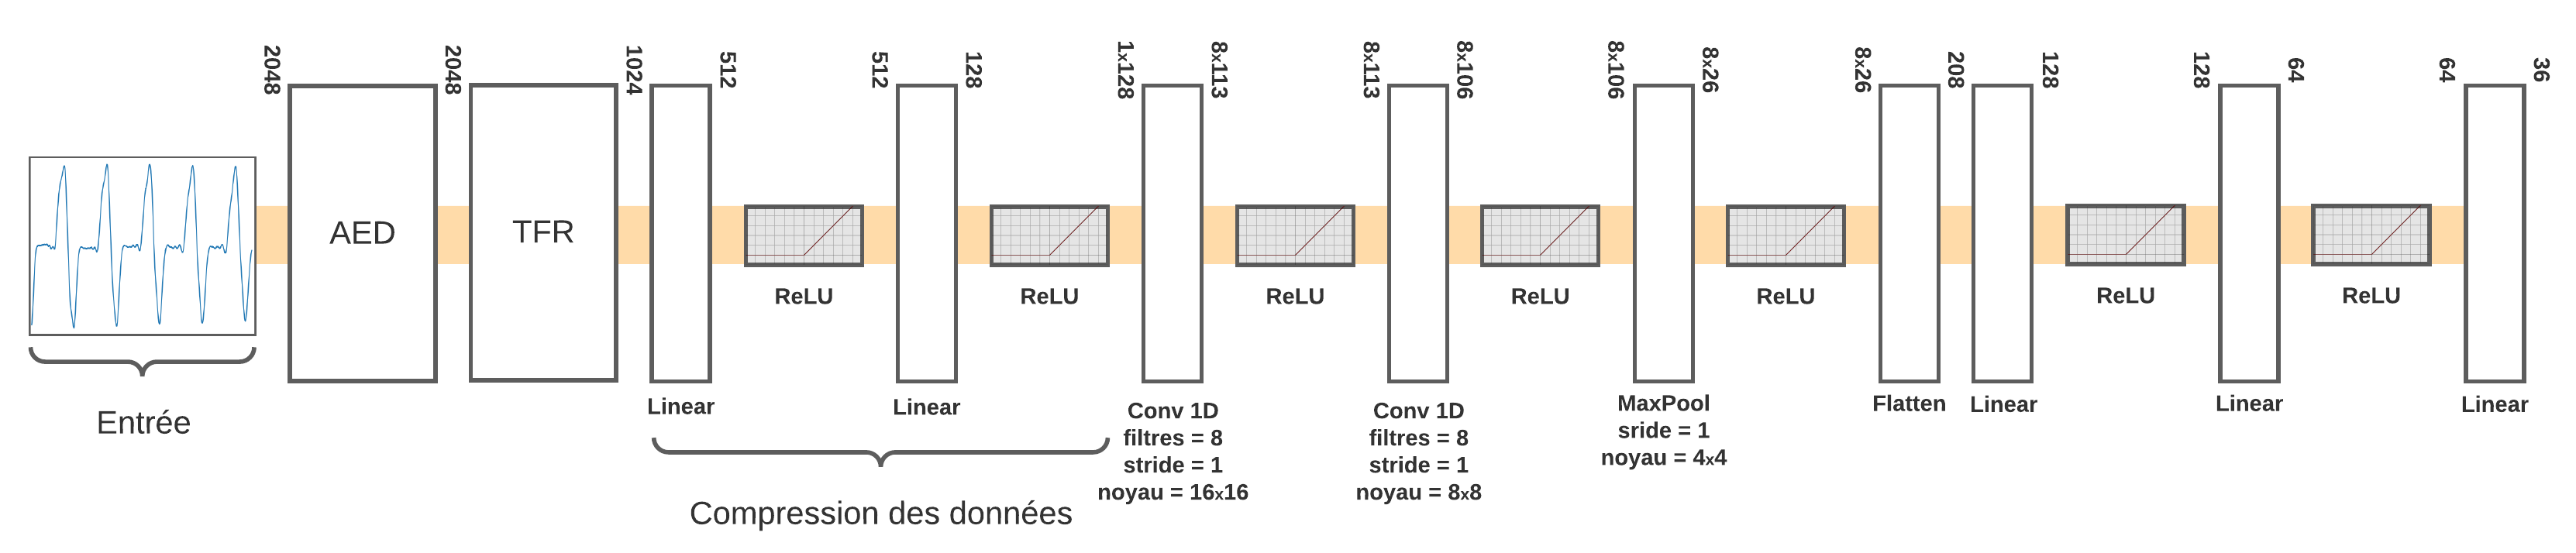
\includegraphics[width=1\linewidth]{cnn_fft}
	\caption[Architecture RNC avec TFR]{Architecture RNC avec TFR. Source : Réalisé par \textsc{Küenzi} Jean-Daniel}
	\label{fig:cnn_fft}
\end{figure}

\subsection{Matrice de confusion sur l'ensemble de validation}
\label{subsec:6.2.2}

La matrice de confusion suivante a été réalisée avec le modèle utilisant une fenêtre de 2048 échantillons.

\begin{figure}[H]
	\centering
	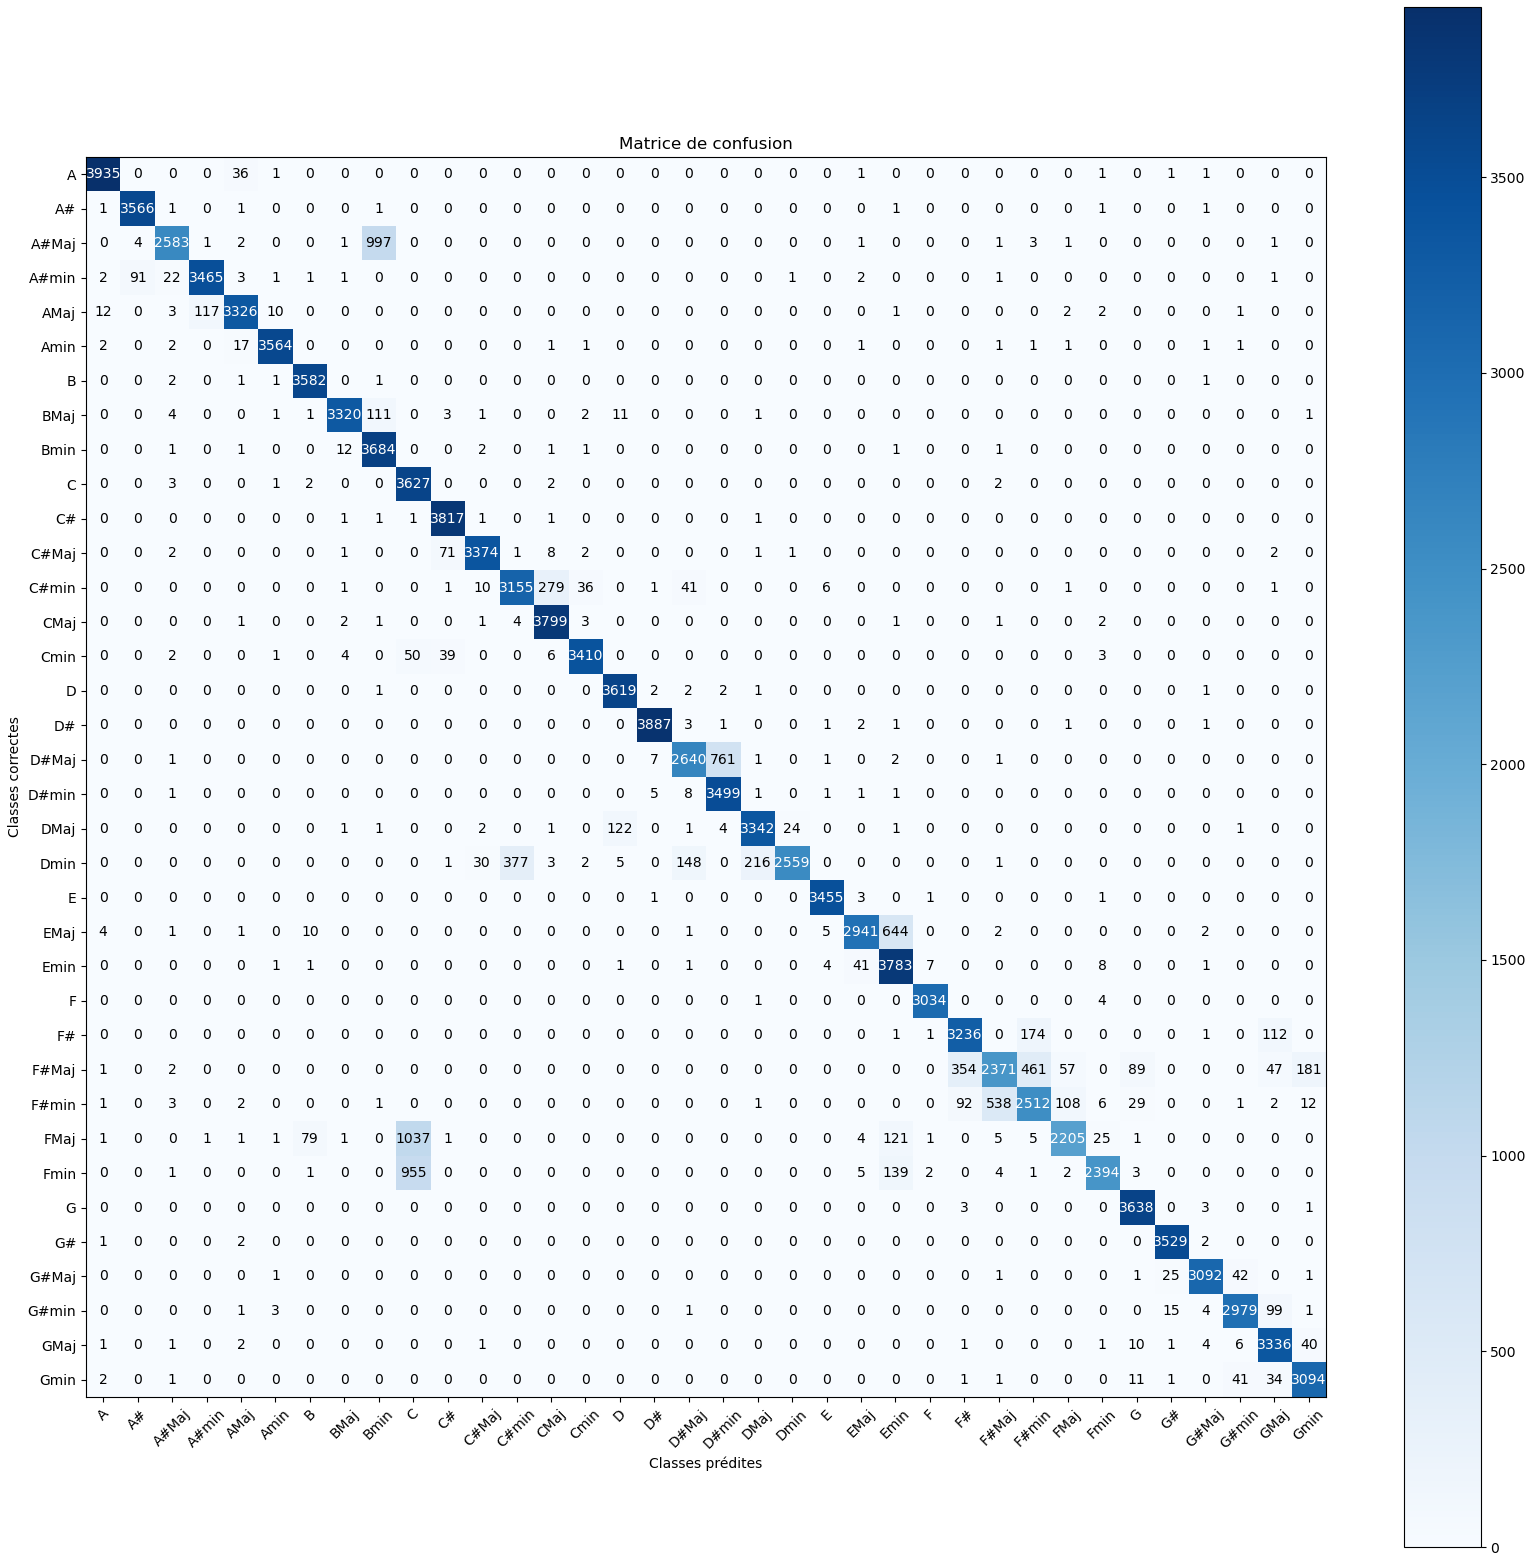
\includegraphics[width=1\linewidth]{cm_cnn_fft}
	\caption[Matrice de confusion pour l'architecture RNC avec TFR]{Matrice de confusion pour l'architecture RNC avec TFR. Source : Réalisé par \textsc{Küenzi} Jean-Daniel}
	\label{fig:cm_cnn_fft}
\end{figure}

Pour la matrice de confusion de l'architecture \gls{rnc}, on peut tout d'abord constater le même problème que celui décrit dans la \autoref{subsec:6.1.2}. Mais en plus de cela, on remarque que le modèle s'est plus trompé sur les différentes notes et accords. Notamment Dmin dont il a prédit certains exemples comme étant C\sh Maj. On peut donc observer la structure des deux accords pour essayer de comprendre ce qui s'est passé.

\begin{table}[H]
	\centering{
		\begin{tabular}{|l|c|c|}
			\hline
			& \textbf{C\sh Maj} & \textbf{Dmin} \\
			\hline
			Fondamentale & C\sh & D \\
			\hline
			Tierce & F & F \\
			\hline
			Quinte juste & G\sh & A \\
			\hline 
		\end{tabular}
		\caption[Comparaison de l'accord C\sh Maj et Dmin]{Comparaison de l'accord C\sh Maj et Dmin. Source : Réalisé par \textsc{Küenzi} Jean-Daniel}
		\label{tab:almost_same_chord}
	}
\end{table}

Dans mon ensemble de données, il se trouve que C\sh Maj et Dmin sont dans la même octave, on peut donc en déduire qu'ils partagent la même tierce, à savoir F mais aussi que la fondamentale et la quinte de l'accord Dmin sont $1/2$ ton plus élevé que celle de l'accord C\sh Maj. On peut dès lors représenter ces notes par leurs valeurs de fréquences (en Hertz) plutôt que leurs noms afin d'observer les écarts entre les fréquences de ces deux accords.

\begin{table}[H]
	\centering{
		\begin{tabular}{|l|c|c|c|}
			\hline
			& \textbf{C\sh Maj} & \textbf{Dmin} & \textbf{Écart en [Hz]} \\
			\hline
			Fondamentale [Hz] & 138.59 & 146.83 & 8.24 \\
			\hline
			Tierce [Hz] & 349.23 & 349.23 & 0.00 \\
			\hline
			Quinte juste [Hz] & 207.65 & 220 & 12.35 \\
			\hline 
		\end{tabular}
		\caption[Comparaison de l'accord C\sh Maj et Dmin sous forme de fréquences]{Comparaison de l'accord C\sh Maj et Dmin sous forme de fréquences. Source : Réalisé par \textsc{Küenzi} Jean-Daniel. A partir de \textit{Wikipedia}, ref. URL11}
		\label{tab:almost_same_chord_hz}
	}
\end{table}

Finalement cette erreur n'est pas si grave et plutôt intéressante, car on voit bien que les deux accords sont relativement proches et que peu de Hertz suffisent à les différencier. On comprend donc bien qu'avec une fenêtre de 2048 échantillons, soit une résolution fréquentielle de \textasciitilde$21.53$[Hz], nous ne sommes pas du tout précis lorsque nous effectuons la \gls{tfr} et que dans ce cas, le modèle a de la peine à bien différencier les deux accords à cause de leurs proximités. Vous pouvez retrouver en annexe (voir \autoref{app:5}) la comparaison du spectre de Fourier entre C\sh Maj et Dmin.

\subsection{Entrainements pour différentes tailles de fenêtres}

\begin{table}[H]
	\centering{
		\begin{tabular}{c l c c}
			\hline
			\multicolumn{4}{c}{\textbf{RNC avec \gls{tfr}}} \\
			\multicolumn{4}{c}{epochs = 50, $\eta$ = 0.005, nombre d'entrainements = 10} \\
			\hline
			\textbf{Nombre d'échantillons} & \textbf{Données} & \textbf{Précision moyenne \%} & \textbf{Ecart type \%} \\
			\hline
			\multirow{2}{*}{1024} & Entrainement & 99.00 & 0.35 \\
			& Validation & 86.08 & 0.78 \\
			\hline
			\multirow{2}{*}{2048} & Entrainement & 99.81 & 0.01 \\
			& Validation & 93.37 & 0.42 \\
			\hline
			\multirow{2}{*}{3072} & Entrainement & 99.82 & 0.06 \\
			& Validation & 94.30 & 0.39 \\
			\hline
			\multirow{2}{*}{4096} & Entrainement & 99.91 & 0.02 \\
			& Validation & 93.51 & 0.13 \\
			\hline
		\end{tabular}
		\caption[Entrainement de l'architecture RNC avec TFR]{Entrainement de l'architecture RNC avec TFR. Source : Réalisé par \textsc{Küenzi} Jean-Daniel}
		\label{tab:rnc_with_tfr}
	}
\end{table}

En observant ces résultats, on constate tout d'abord que l'architecture \gls{rnc} avec \gls{tfr} est légèrement moins précise que l'architecture \gls{pmc} avec \gls{tfr}. On remarque aussi qu'une fenêtre de 2048 échantillons n'est pas suffisante, l'architecture \gls{rnc} a plutôt besoin d'une fenêtre de 3072 pour atteindre sa précision maximale. Même si les résultats sont légèrement moins bons que l'architecture \gls{pmc} avec \gls{tfr}, ils restent néanmoins plutôt corrects et intéressants. Donc 3072 échantillons semblent une bonne de taille fenêtre pour avoir une bonne précision, nous avons une résolution fréquentielle de \textasciitilde$14.35$[Hz] et une résolution temporelle de \textasciitilde$0.069$[s]. Toutefois, sa résolution temporelle est un peu élevée et la latence visuelle se fait un peu ressentir lors de l'utilisation en temps réel. Généralement, en dessous de \textasciitilde0.025[s] l'œil ne perçoit pas la latence. Il vaut mieux donc utiliser une fenêtre de 2048 échantillons même si nous perdons un peu en précision afin de ne pas gêner l'utilisation en temps réel.

\begin{table}[H]
	\centering{
		\begin{tabular}{c l c c}
			\hline
			\multicolumn{4}{c}{\textbf{RNC sans \gls{tfr}}} \\
			\multicolumn{4}{c}{epochs = 50, $\eta$ = 0.005, nombre d'entrainements = 10} \\
			\hline
			\textbf{Nombre d'échantillons} & \textbf{Données} & \textbf{Précision moyenne \%} & \textbf{Ecart type \%} \\
			\hline
			\multirow{2}{*}{1024} & Entrainement & 99.49 & 0.18 \\
			& Validation & 90.28 & 0.41 \\
			\hline
			\multirow{2}{*}{2048} & Entrainement & 99.84 & 0.04 \\
			& Validation & 91.51 & 0.42 \\
			\hline
			\multirow{2}{*}{3072} & Entrainement & 99.89 & 0.05 \\
			& Validation & 90.78 & 0.30 \\
			\hline
			\multirow{2}{*}{4096} & Entrainement & 99.85 & 0.06 \\
			& Validation & 89.54 & 0.58 \\
			\hline
		\end{tabular}
		\caption[Entrainement de l'architecture RNC sans TFR]{Entrainement de l'architecture RNC sans TFR. Source : Réalisé par \textsc{Küenzi} Jean-Daniel}
		\label{tab:rnc_without_tfr}
	}
\end{table}

En observant ces résultats, on constate tout d'abord que l'architecture \gls{rnc} sans \gls{tfr} est moins précise que l'architecture \gls{pmc} sans \gls{tfr}. On constate également que la fenêtre avec 2048 échantillons est celle qui a donné les meilleurs résultats. Finalement on peut observer qu'à partir de la fenêtre avec 2048 échantillons, l'augmentation du nombre d'échantillons fait chuter la précision du modèle. Cela est surement dû aux mêmes raisons que pour l'architecture \gls{pmc} sans \gls{tfr}.

Finalement, l'architecture convolutive est celle qui a donné les moins bons résultats, c'est pourquoi je ne l'ai pas retenue comme ma solution finale. Toutefois, ses résultats restent corrects et encourageants, cette architecture n'est donc pas à négliger.
% !TeX spellcheck = fr_FR
\chapter{Chapitre 7 : Résultats}
\label{chap:7}

\section{AED}
\label{sec:7.1}

\subsection{Entrainements pour différentes tailles de fenêtres}

\begin{table}[H]
	\centering{
		\begin{tabular}{c l c c}
			\hline
			\multicolumn{4}{c}{\textbf{AED}} \\
			\multicolumn{4}{c}{epochs = 50, $\eta$ = 0.005, nombre d'entrainements = 10} \\
			\hline
			\textbf{Nombre d'échantillons} & \textbf{Données} & \textbf{Valeur de perte moyenne} & \textbf{Ecart type} \\
			\hline
			\multirow{2}{*}{1024} & Entrainement & 0.0094 & 0.0038 \\
			& Validation & 0.0096 & 0.0076 \\
			\hline
			\multirow{2}{*}{2048} & Entrainement & 0.0096 & 0.0018 \\
			& Validation & 0.0083 & 0.0014 \\
			\hline
			\multirow{2}{*}{3072} & Entrainement & 0.0088 & 0.0025 \\
			& Validation & 0.0084 & 0.0014 \\
			\hline
			\multirow{2}{*}{4096} & Entrainement & 0.0089 & 0.0010 \\
			& Validation & 0.0085 & 0.0013 \\
			\hline
		\end{tabular}
		\caption[Entrainement de l'AED pour différentes tailles de fenêtres]{Entrainement de l'AED pour différentes tailles de fenêtres. Source : Réalisé par \textsc{Küenzi} Jean-Daniel}
		\label{tab:aed_training}
	}
\end{table}

Lorsqu'on observe ces résultats, on remarque que l'\gls{aed} a eu plus de peine à reconstruire les données non bruitées quand on utilise une fenêtre de 1024 échantillons. Cela peut être dû au fait que le bruit blanc gaussien ajouté est trop fort pour la taille de cette fenêtre. Toutefois, la valeur de perte moyenne reste assez faible et les données bruitées sont plutôt bien reconstruites sans le bruit. On remarque aussi qu'à partir d'une fenêtre de 2048 échantillons, l'augmentation du nombre d'échantillons ne fait pas augmenter cette valeur de perte, ce qui est positif, une valeur de perte plus grande veut dire une reconstruction des données moins bonne.

\subsection{Reconstruction d'une donnée non bruitée}

Dans cette partie, nous allons voir comment l'\gls{aed} se comporte lorsqu'il reçoit une donnée non bruitée en entrée. Pour cet exemple j'ai joué un A à 110 [Hz] avec le plectre.

\begin{figure}[H]
	\centering
	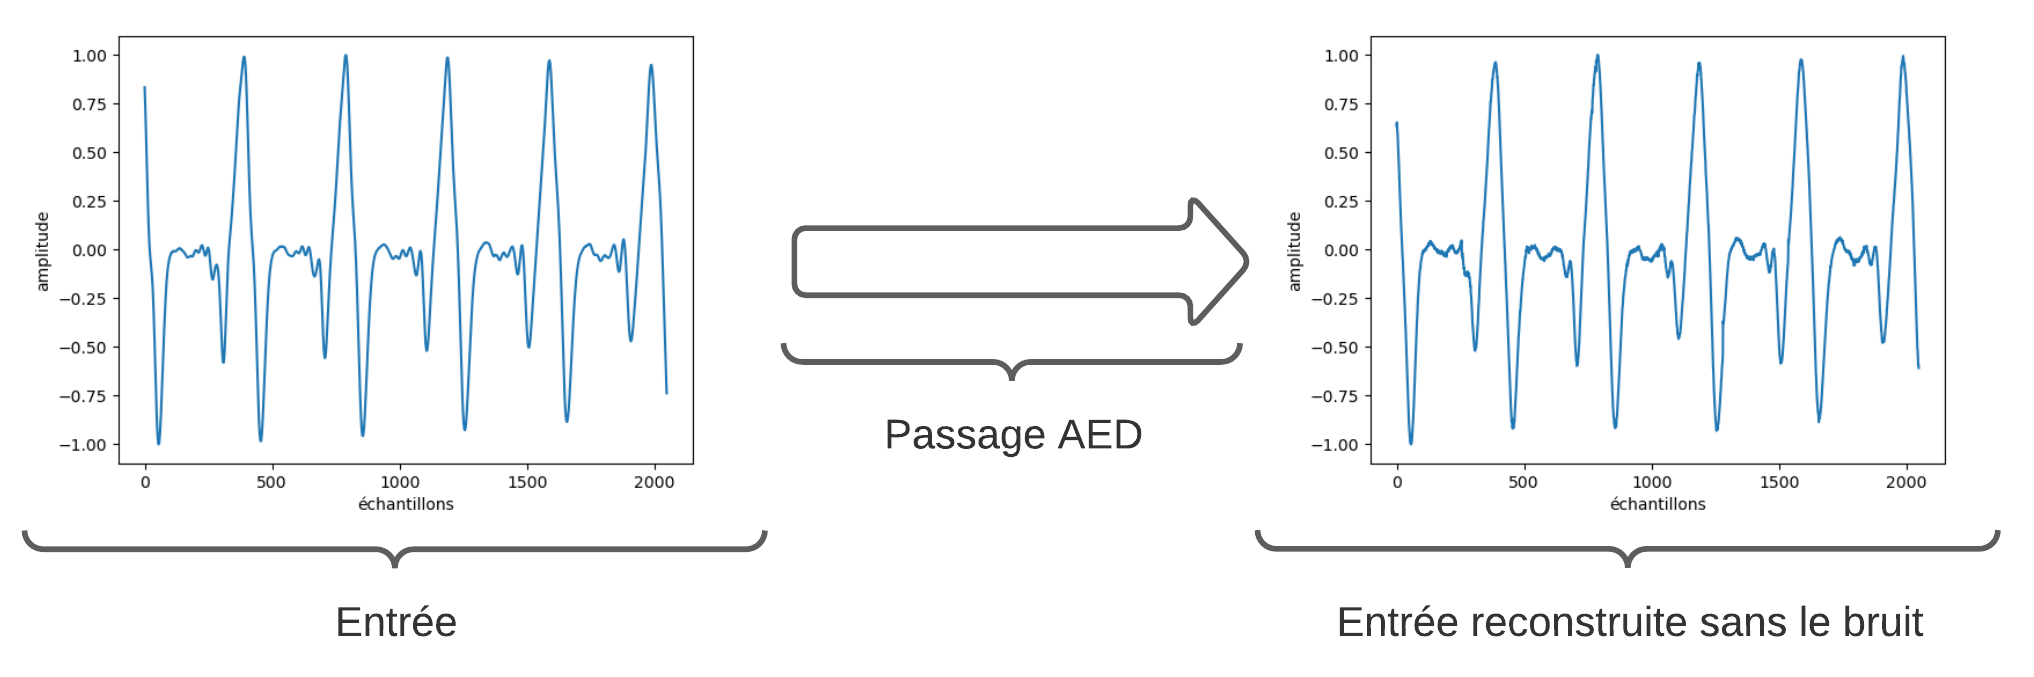
\includegraphics[width=1\linewidth]{aed_clean_denoise}
	\caption[Reconstruction d'un A à 110 Hertz non bruité]{Reconstruction d'un A à 110 [Hz] non bruité. Source : Réalisé par \textsc{Küenzi} Jean-Daniel}
	\label{fig:aed_clean_denoise}
\end{figure}

On peut constater que le signal à la sortie de l'\gls{aed} est quasiment le même qu'à l'entrée. Comme le signal d'entrée n'était pas bruité, l'\gls{aed} s'est uniquement contenté de reconstruire le même signal. On peut retrouver les différents pics du signal aux bons endroits, et l’on remarque entre chaque pic qu'il y a une très légère différence entre l'entrée et la sortie.

\subsection{Reconstruction d'une donnée avec du bruit blanc gaussien}

Dans cette partie, nous allons voir comment l'\gls{aed} se comporte lorsqu'il reçoit une donnée bruitée en entrée. Pour cet exemple, il s'agit du même A à 110 [Hz] de l'exemple précédent, mais avec du bruit blanc gaussien ajouté. Le bruit blanc gaussien qui a été ajouté a une moyenne de zéro et un écart type de zéro virgule trois. Ce bruit ajouté est comparable à un souffle constant assez fort.

\begin{figure}[H]
	\centering
	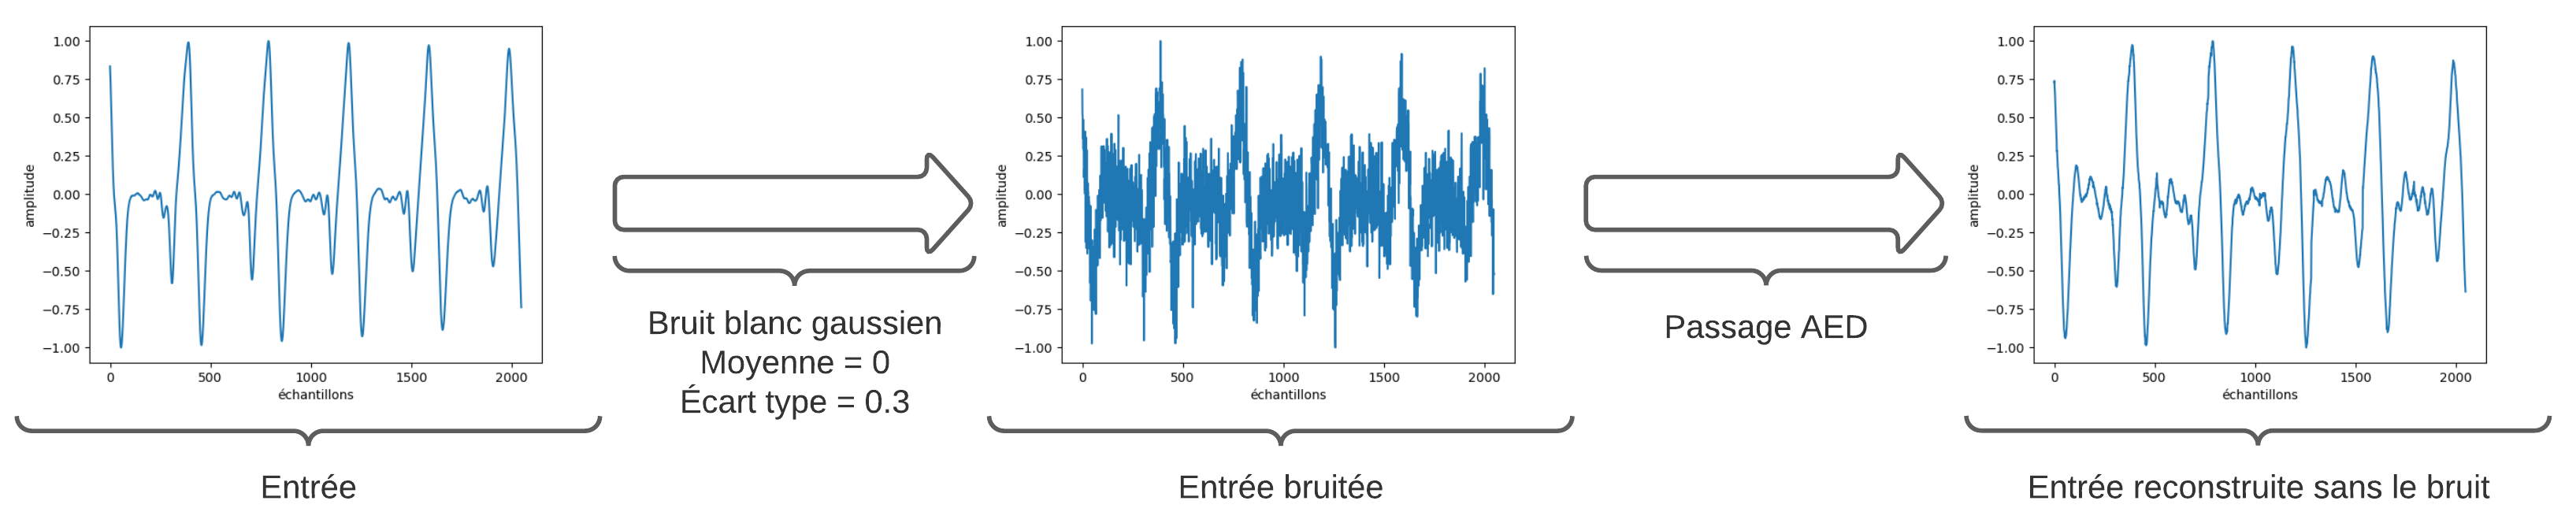
\includegraphics[width=1\linewidth]{aed_denoise}
	\caption[Reconstruction d'un A à 110 Hertz avec du bruit blanc gaussien]{Reconstruction d'un A à 110 [Hz] avec du bruit blanc gaussien. Source : Réalisé par \textsc{Küenzi} Jean-Daniel}
	\label{fig:aed_denoise}
\end{figure}

On peut constater que le signal à la sortie de l'\gls{aed} est semblable à celui qui est à l'entrée, mais légèrement différent. Comme le signal d'entrée était bruité, l'\gls{aed} à correctement extrait les caractéristiques nécessaires pour reconstruire le signal sans le bruit. On constate également que le signal reconstruit est quasiment le même que le signal qui se trouve en entrée. On peut retrouver les différents pics du signal aux bons endroits, et on remarque entre chaque pic, qu'il y a une différence entre l'entrée et la sortie.

\subsection{Reconstruction d'une donnée avec du gain}

Dans cette partie nous allons voir comment l'\gls{aed} se comporte lorsqu'il reçoit une donnée bruitée avec du gain en entrée. Pour cet exemple j'ai joué un Dmin avec la basse à \textasciitilde146,83[Hz]. Pour ajouter le gain dans le signal, j'ai utilisé un amplificateur \textsc{Aslin Dane AG-15R}. Toutefois, l'amplificateur étant assez vieux je n'ai pas réussi à trouver sa fiche technique et donc de ce fait, pas pu déterminer le gain ajouter en décibels.

\begin{figure}[H]
	\centering
	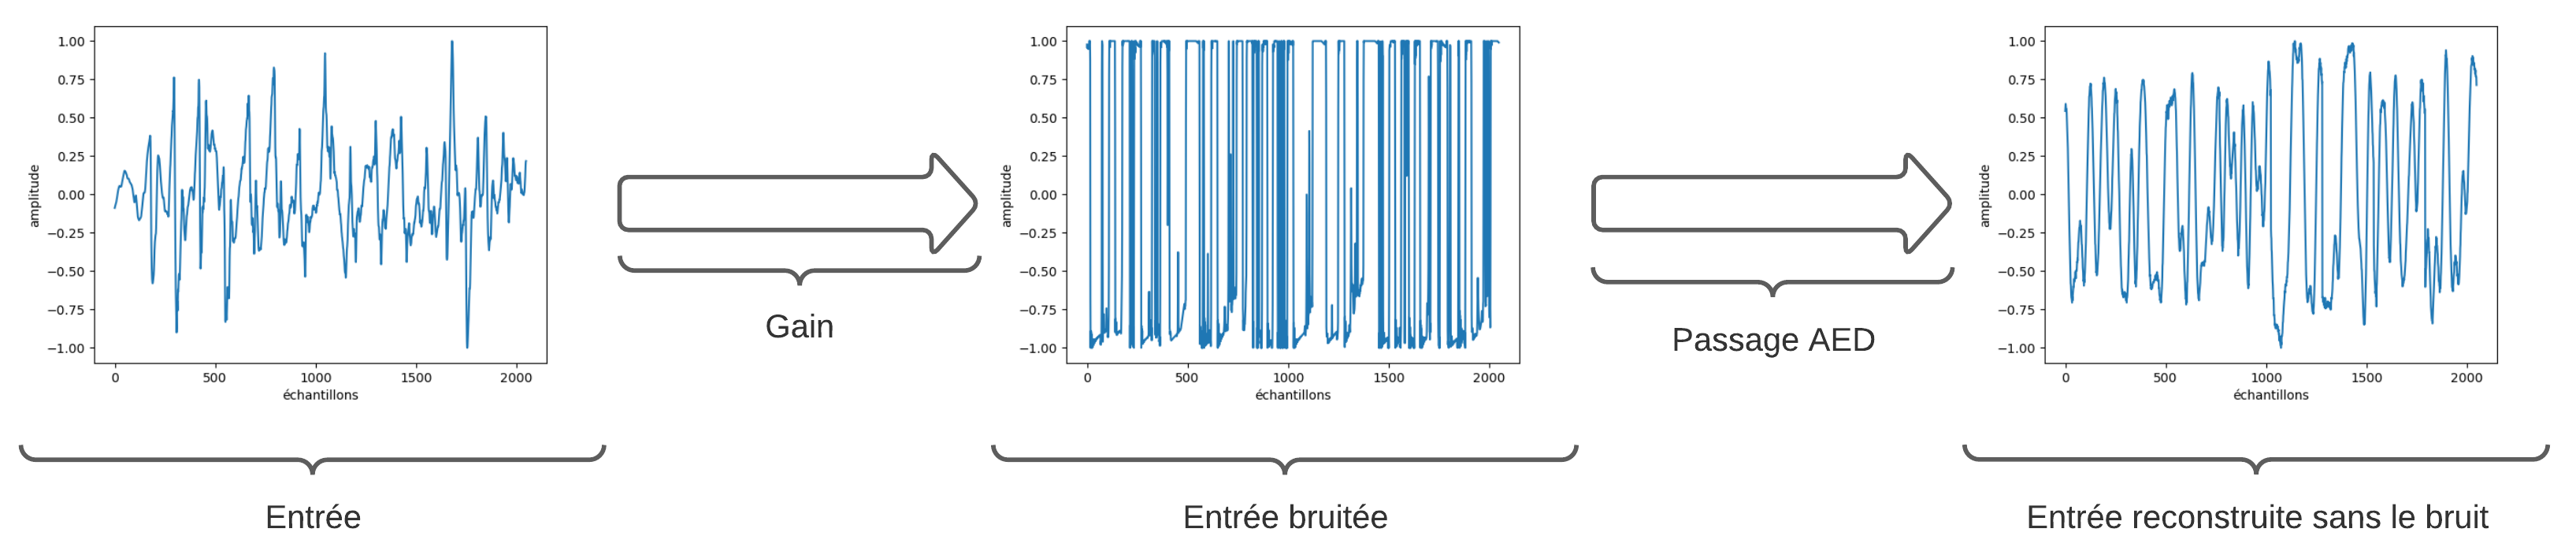
\includegraphics[width=1\linewidth]{aed_gain_denoise}
	\caption[Reconstruction d'un Dmin avec du gain]{Reconstruction d'un Dmin avec du gain. Source : Réalisé par \textsc{Küenzi} Jean-Daniel}
	\label{fig:aed_gain_denoise}
\end{figure}

On peut constater que le signal à la sortie de l'\gls{aed} est très différent de celui qui est en entrée. Cela est normal et compréhensible, l'\gls{aed} a été entrainé à reconstruire les données sans du bruit blanc gaussien et non pas à reconstruire les données sans du gain. De plus, on observe que le gain ajouté est vraiment fort et qu'il déforme énormément le signal, il en devient presque carré. Toutefois, on remarque que la reconstruction des données est assez intéressante,  l'\gls{aed} a réduit les amplitudes et rendu le signal moins carré. J'ai également observé que l'utilisation de l'\gls{aed} permettait au modèle de prédire beaucoup plus facilement l'accord avec du gain lors de l'utilisation en temps réel. Lorsque je n'utilisais pas l'\gls{aed} et que le modèle prenait le signal brut avec le gain, le modèle prédisait surtout la quinte et la tierce mais rarement l'accord. Avec l'\gls{aed}, il avait beaucoup plus de facilité à prédire l'accord.

\section{LSTMB}
\label{sec:7.2}

\subsection{Matrice de confusion sur l'ensemble de validation}

La matrice de confusion suivante a été réalisée avec le modèle utilisant une fenêtre de 2048 échantillons.

\begin{figure}[H]
	\centering
	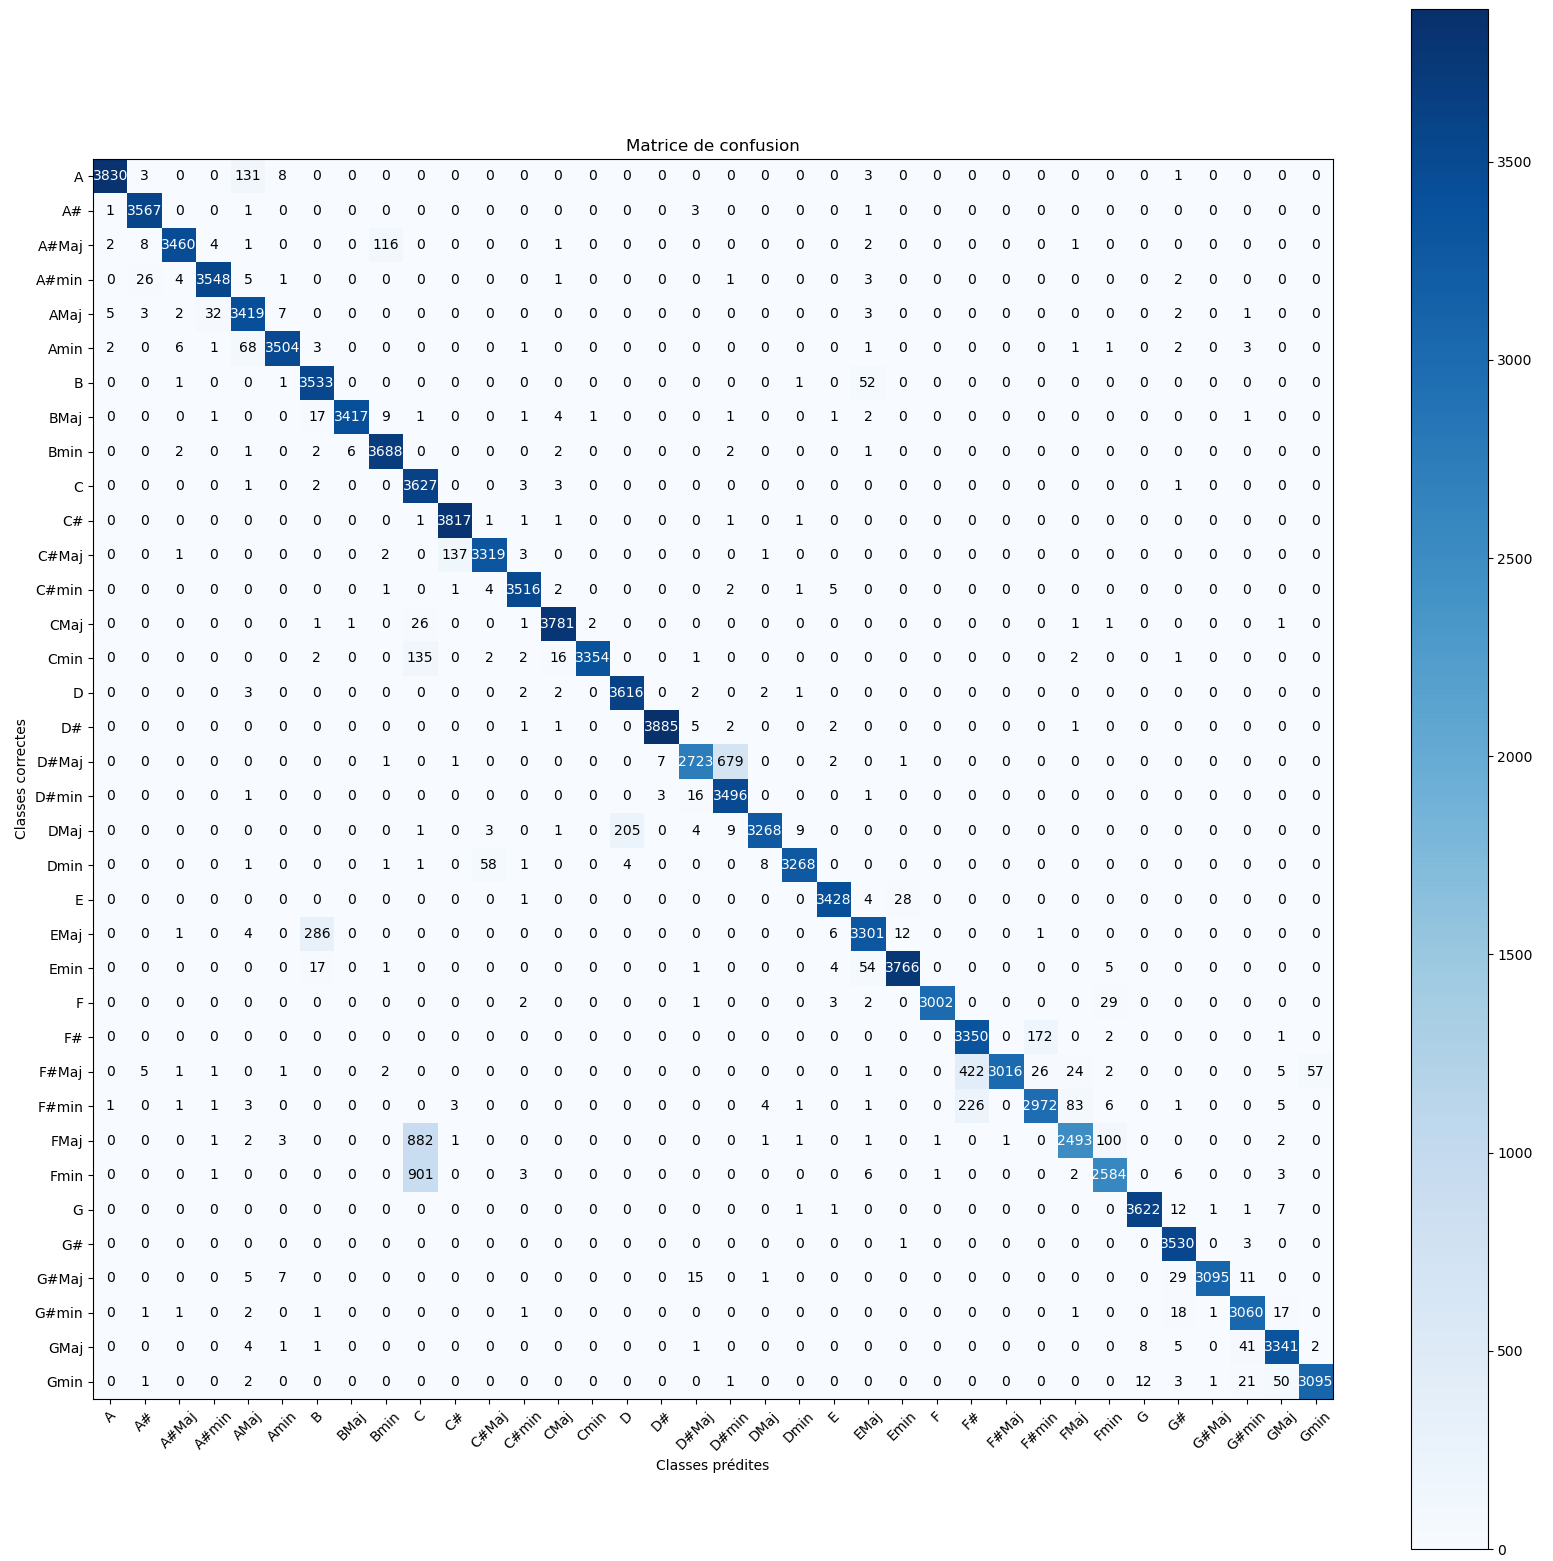
\includegraphics[width=1\linewidth]{cm_lstmb_fft}
	\caption[Matrice de confusion pour l'architecture LSTMB avec TFR]{Matrice de confusion pour l'architecture LSTMB avec TFR. Source : Réalisé par \textsc{Küenzi} Jean-Daniel}
	\label{fig:cm_lstmb_fft}
\end{figure}

Tout d'abord, lorsque l'on observe la matrice de confusion, on peut constater le même problème qui est décrit dans la \autoref{subsec:6.1.2} de la \autoref{sec:6.1}, c'est-à-dire que le modèle a prédit certaine composante des accords, comme la fondamentale, la tierce ou la quinte. En fait cela n'est pas réellement une erreur et relève plutôt d'une imperfection dans l'ensemble de validation. Aussi on remarque que la grande majorité des données sont correctement classées (visible par la diagonale qui traverse la matrice). Toutefois, le modèle confond parfois les accords majeurs et mineurs. 

Ainsi, comme décrit dans la \autoref{subsec:6.2.2} de la \autoref{sec:6.2}, il confond les accords qui sont assez proches. C'est notamment le cas avec A\sh Maj que le modèle a confondu avec un Bmin. Finalement les résultats de l'architecture \gls{lstmb} avec \gls{tfr} sont très similaires aux résultats obtenus avec l'architecture \gls{pmc} avec \gls{tfr} et sont dans leurs globalités excellents.

\subsection{Entrainements pour différentes tailles de fenêtres}

\begin{table}[H]
	\centering{
		\begin{tabular}{c l c c}
			\hline
			\multicolumn{4}{c}{\textbf{LSTMB avec \gls{tfr}}} \\
			\multicolumn{4}{c}{epochs = 50, $\eta$ = 0.005, nombre d'entrainements = 10} \\
			\hline
			\textbf{Nombre d'échantillons} & \textbf{Données} & \textbf{Précision moyenne \%} & \textbf{Ecart type \%} \\
			\hline
			\multirow{2}{*}{1024} & Entrainement & 99.53 & 0.11 \\
			& Validation & 85.32 & 0.45 \\
			\hline
			\multirow{2}{*}{2048} & Entrainement & 99.81 & 0.01 \\
			& Validation & 95.51 & 0.33 \\
			\hline
			\multirow{2}{*}{3072} & Entrainement & 99.88 & 0.02 \\
			& Validation & 94.88 & 0.23 \\
			\hline
			\multirow{2}{*}{4096} & Entrainement & 99.91 & 0.01 \\
			& Validation & 94.30 & 0.26 \\
			\hline
		\end{tabular}
		\caption[Entrainement de l'architecture LSTMB avec TFR]{Entrainement de l'architecture LSTMB avec TFR. Source : Réalisé par \textsc{Küenzi} Jean-Daniel}
		\label{tab:lstm_with_tfr}
	}
\end{table}

Lorsque l'on observe ces résultats, le premier constat est le même que pour l'architecture \gls{pmc} et \gls{rnc} avec \gls{tfr}. Une fenêtre de 1024 échantillons n'est pas suffisante pour permettre une bonne prédiction des classes. Avec 1024 échantillons, nous avons une résolution fréquentielle de \textasciitilde$43.06$[Hz]. Nous ne sommes donc pas du tout précis et cela va fortement impacter le modèle lors de la prédiction. Ensuite, on remarque que l'architecture \gls{lstmb} avec \gls{tfr} nous a donné les meilleurs résultats avec une fenêtre de 2048 échantillons. Comme précisé dans la \autoref{sec:3.7}, les cellules \gls{lstm} sont très efficaces dans le traitement de données chronologiques. Finalement, on remarque qu'à partir de la fenêtre avec 2048 échantillons, augmenter le nombre d'échantillons fait chuter la précision. Cela peut être en partie dû à la réduction de la taille de l'ensemble de données ainsi qu'au problème évoqué dans la \autoref{subsec:6.1.2}. 

\begin{table}[H]
	\centering{
		\begin{tabular}{c l c c}
			\hline
			\multicolumn{4}{c}{\textbf{LSTMB sans \gls{tfr}}} \\
			\multicolumn{4}{c}{epochs = 50, $\eta$ = 0.005, nombre d'entrainements = 10} \\
			\hline
			\textbf{Nombre d'échantillons} & \textbf{Données} & \textbf{Précision moyenne \%} & \textbf{Ecart type \%} \\
			\hline
			\multirow{2}{*}{1024} & Entrainement & 99.69 & 0.15 \\
			& Validation & 91.49 & 0.22 \\
			\hline
			\multirow{2}{*}{2048} & Entrainement & 99.91 & 0.02 \\
			& Validation & 92.45 & 0.54 \\
			\hline
			\multirow{2}{*}{3072} & Entrainement & 99.94 & 0.05 \\
			& Validation & 92.21 & 0.15 \\
			\hline
			\multirow{2}{*}{4096} & Entrainement & 99.94 & 0.03 \\
			& Validation & 91.25 & 0.16 \\
			\hline
		\end{tabular}
		\caption[Entrainement de l'architecture LSTMB sans TFR]{Entrainement de l'architecture LSTMB sans TFR. Source : Réalisé par \textsc{Küenzi} Jean-Daniel}
		\label{tab:lstm_without_tfr}
	}
\end{table}

En observant ces résultats, on constate tout d'abord qu'ils sont légèrement moins bons que ceux de l'architecture avec \gls{tfr}, mais l'on remarque aussi que la fenêtre de 2048 échantillons donne le meilleur résultat entre les trois architectures sans \gls{tfr}. Néanmoins, ces résultats sont très encourageants, on remarque que le modèle a une assez bonne précision avec les données discrètes. On remarque également qu'à partir de la fenêtre avec 2048 échantillons, l'augmentation du nombre d'échantillons fait légèrement chuter la précision du modèle. Cela peut être dû au nombre d'epochs qui n'est plus suffisant pour laisser au réseau le temps de bien converger ou à la réduction de la taille de l'ensemble de données ainsi qu'au problème évoqué dans la \autoref{subsec:6.1.2}.

\section{Ressenti d'utilisation en temps réel}
\label{sec:7.3}

Lors de mon utilisation en temps réel, j'ai tout d'abord constaté que les accords et notes joués étaient correctement prédits. De plus, j'ai mesuré le temps passé à traverser le modèle, avec une utilisation en CPU, depuis le moment où nous avons nos 2048 échantillons jusqu'à l'obtention de la prédiction de l'accord ou de la note. En moyenne, cela prend entre trois et quatre millisecondes, nous sommes donc bien en dessous des cinq millisecondes visées. De plus, lors de l'utilisation en temps réel le modèle prend en entrée une fenêtre de 2048 échantillons, ce qui représente une durée de \textasciitilde$0.046$[s]. Mais j'utilise une taille de chevauchement de 1024 échantillons, soit \textasciitilde$0.023$[s], ce qui fait que la toutes premières fenêtre aura une latence de \textasciitilde$0.046$[s], mais les autres fenêtres auront une latence divisée par un facteur de deux grâce au chevauchement, soit une latence de \textasciitilde$0.023$[s]. En somme, on utilise les 1024 derniers échantillons de la fenêtre à l'instant $t-1$ pour construire notre fenêtre à l'instant $t$. La latence visuelle est donc presque imperceptible et l'impression du temps réel se fait bien ressentir.

Ensuite, concernant l'attaque, elle est légèrement visible au début de la prédiction, c'est-à-dire lors de la première fenêtre. Elle est donc uniquement visible pendant \textasciitilde$0.046$[s] ce qui n'est pas très gênant.

J'ai également constaté que le modèle ne semble pas avoir de problèmes avec les changements de phases dans les signaux. J'ai notamment testé différentes techniques de legato (hammer-on, pull-off, etc.), c'est-à-dire que j'ai lié les notes jouées sans laisser de silence entre elles et sans réattaquer la corde avec le plectre ou le doigt. Ce qui est intéressant avec ces techniques, c'est qu'elles vont créer un changement de phase brusque dans le signal, étant donné que l'on va par exemple passer d'un F à un F\sh\,ou un G de manière instantanée.

J'ai aussi testé différends bends (technique à la guitare), c'est-à-dire que j'ai volontairement tiré latéralement la corde sur laquelle je jouais pour augmenter sa vibration et ainsi atteindre une note différente (par exemple pour atteindre un G depuis un F). Cette technique est très intéressante, car elle nous fait passer par toutes les fréquences entre la note de base et la note visée. Par exemple pour passer d'un F à un G dans la même octave, nous allons passer par toutes la bande de fréquence [174.61; 196.00]. C'est donc un bon moyen de déterminer si le modèle est sensible aux changements de phases.

J'ai constaté de plus que le modèle a plus de facilité à détecter les notes que les accords, ce qui est compréhensible étant donné que le spectre de Fourier d'une note, et donc d'un signal, est beaucoup moins complexe que celui d'un accord qui est une agrégation de plusieurs notes, et donc signaux différents.

Pour finir, j'ai rajouté la fondamentale et la quinte plusieurs fois à l'octave dans l'accord et donc de ne plus jouer un accord à trois sons, comme au départ, mais de jouer un accord avec six sons. Par exemple l'accord EMaj est joué avec les notes dans l'ordre suivant :

\begin{table}[H]
	\centering{
		\begin{tabular}{|l|c|c|c|}
			\hline
			\multicolumn{4}{|c|}{\textbf{A Majeur}} \\
			\hline
			& \textbf{Notes} & \textbf{Octave} & \textbf{Fréquence en [Hz]} \\
			\hline
			Fondamentale & E & 1 & 82.41 \\
			\hline
			Quinte juste & B & 1 & 123.47 \\
			\hline
			Fondamentale & E & 2 & 164.81 \\
			\hline
			Tierce majeure & G\sh & 2 & 207.65 \\
			\hline
			Quinte & B & 2 & 246.94 \\
			\hline
			Fondamentale & E & 3 & 329.63 \\
			\hline 
		\end{tabular}
		\caption[Accord AMaj avec la quinte et la fondamentale sur plusieurs octaves]{Accord AMaj avec la quinte et la fondamentale sur plusieurs octaves. Source : Réalisé par \textsc{Küenzi} Jean-Daniel. A partir de \textit{Wikipedia}, ref. URL11}
		\label{tab:full_amaj}
	}
\end{table}

Le fait de rajouter des composantes comme la fondamentale et la quinte à l'octave ne gêne pas les prédictions du modèle et cela peut s'expliquer par le fait que sur le spectre de Fourier, nous allons retrouver les trois composantes de l'accord à trois sons, à savoir la fondamentale, la tierce et la quinte juste. De plus, comme les composantes rajoutées sont des multiples des trois composantes de bases, cela correspond donc aux partiels harmoniques qui étaient déjà présents sur le spectre, mais cette fois elles seront plus fortes et vont à leurs tours rajouter leur propre partiels harmoniques.

% !TeX spellcheck = fr_FR
\chapter*{Conclusion}
\addcontentsline{toc}{chapter}{Conclusion} % Adding toc entry

% Fonction de rappel
Dans un premier temps, le but de ce travail était de pouvoir détecter automatiquement des accords et notes de guitare à l'aide de différents modèles connexionnistes. Je devais donc mettre en place différentes architectures afin de comparer leurs résultats et je devais également construire mon propre ensemble de données en partant de zéro. Pour ce projet, je devais également considérer les signaux dans le monde discret et dans le monde fréquentiel. Dans un deuxième temps, je devais déterminer si les modèles étaient capables de fonctionner en temps réel.

Nous avons vu au cours de cette thèse que j'ai décidé d'implémenter et tester trois architectures, à savoir l'architecture \gls{pmc}, l'architecture \gls{rnc} et l'architecture \gls{lstmb}. Nous avons pu constater et comparer les résultats de ses trois architectures qui sont très satisfaisants. Bien que l'architecture \gls{rnc} soit celle qui ait fonctionné le moins bien, les résultats restent très corrects. Nous avons également vu que pour passer du monde discret au monde fréquentiel j'ai choisi d'utiliser la \gls{tfr} pour sa simplicité et sa rapidité. Ce qui est un facteur essentiel pour l'utilisation en temps réel. Nous avons pu observer de plus que les modèles utilisant la \gls{tfr} étaient plus efficace que ceux utilisant directement les données discrètes. Néanmoins, les résultats obtenus avec les données discrètes restent très encourageants et intéressants à explorer.

Nous avons vu aussi que j'ai dû mettre en place et construire mon propre ensemble de données. C'était très intéressant, car dans un premier temps j'avais fait mes enregistrements sans matériel spécialisé ce qui avait un impact néfaste sur mon ensemble de données, notamment au niveau du bruit dans le signal, et que cet impact se faisait ressentir sur les performances de mes modèles. J'ai ensuite eu accès à une carte son externe spécialisée dans le traitement audio, ce qui m'a permis, sur la base de mon ancien ensemble de données, d'en reconstruire un nouveau avec des données non bruitées et des structures de fichiers complètement différentes. Avec le nouvel ensemble de données, j'ai pu constater une nette amélioration dans l'entrainement des différents modèles.

Suite à ça, j'ai eu l'idée de construire un \gls{aed} afin de réduire le bruit dans les signaux que je recevais en entrée. Tout le monde n'ayant pas forcément de matériel spécialisé, il était donc nécessaire de pouvoir réduire le bruit avant de faire passer les entrées dans les modèles prédictifs. Cet \gls{aed} peut être aussi utile pour réduire les effets comme le gain, ce qui aide le modèle prédictif à prédire correctement.

Finalement, sur la base de mon ressenti d'utilisation en temps réel, nous avons pu constater que le modèle n’était pas sensible au problème du changement de phase dans les signaux et qu’il prédisait correctement les différents accords et notes joués. Nous avons également constaté que le chevauchement des fenêtres a réduit le temps de latence par deux; à savoir, un temps de latence de \textasciitilde0.023[s], ce qui rend l’utilisation en temps réel très fluide et agréable. De ce fait, le temps de latence visuelle n’est quant à lui presque pas perceptible. De plus, nous avons observé que la solution proposée, à savoir l’architecture \gls{lstmb} avec \gls{tfr} était en moyenne traversée en trois à quatre millisecondes, ce qui est bien inférieur aux cinq millisecondes souhaitées.

% Retour reflexif
En tant que passionné de musique et étant moi-même musicien c'était un réel plaisir de travailler sur ce projet. Les recherches effectuées durant ce travail m'ont apporté beaucoup de connaissances sur les notions mathématiques liées au traitement du signal. Notamment comme la fuite spectrale lors de la \gls{tfr}, l'utilisation de fenêtre pour la réduire et le théorème d'échantillonnage de Nyquist-Shanon. J'ai aussi pu approfondir mes connaissances sur les réseaux de neurones en découvrant les cellules \gls{lstm}, la normalisation par lots, les auto-encodeurs et leurs variantes ainsi que les modèles transformer. J'ai de plus pu constater l'importance et la complexité d'avoir un ensemble de données étudiées et correctement construit et donc l'importance et l'implication des "Data Scientist" dans le domaine de l'\gls{ia}. Mais ce travail m'a surtout permis de percevoir la musique dans un contexte purement physique et mathématique et de comprendre réellement ce qu'est la musique à la base.

% Ouverture
% Partie sur d'autres fonction mathématiques
Bien que la \gls{tfr} nous ait donné de bons résultats sur notre ensemble de données, il pourrait y avoir un problème avec la résolution fréquentielle. En effet, plus on descend dans les basses fréquences et plus la hauteur des notes (c'est-à-dire leur fréquence) est rapprochée (1[Hz] peut suffire à différencier un C d'un C\sh). Inversement, plus on monte dans les hautes fréquences, plus la hauteur des notes est éloignée (1[kHz] peut suffire à différencier un C d'un C\sh). On remarque donc que dans les basses fréquences nous avons besoin d'une plus grande taille de fenêtre que dans les hautes fréquences. Mais la \gls{tfr} utilise une taille fixe. Il serait donc intéressant de voir si l'on peut faire varier cette taille de fenêtre automatiquement ou utiliser d'autres fonctions comme la \gls{tfct}, la Transformée en Ondelette ou encore la \gls{tqc} et de voir si cela améliore la précision des différents modèles.

% Partie sur l'AED dans le monde des fréquences
On peut voir que j'ai construit mon \gls{aed} pour qu'il fonctionne dans le monde temporel (avec le signal discret). Il pourrait être intéressant de le considérer dans le monde des fréquences. Ainsi, on pourrait voir si la reconstruction des données non bruitées est plus efficace et plus rapide.

% Partie sur l'augmentation du dataset
Actuellement, l'ensemble de données créé se repose uniquement sur les accords à trois sons mineurs et majeurs ainsi que les notes sur l'accordage standard de la guitare. Dans un premier temps, augmenter l'ensemble de données en rajoutant des accords septièmes, diminués et augmentés pourrait permettre de voir si les architectures actuelles sont suffisantes pour différencier correctement les différents accords et notes. Ensuite, il serait intéressant de continuer l'ensemble de données dans d'autres types d'accordages afin de généraliser le problème et les modèles.

% Partie sur le transfer learning
Un autre point important est que l'ensemble de données actuel, bien qu'il soit petit, m'a pris beaucoup de temps à faire. On imagine donc bien que pour un ensemble de données qui contiendrait plusieurs types d'accords et d'accordages cela deviendrait trop lourd à construire. On pourrait donc essayer d'utiliser un modèle génératif et de faire de l'Apprentissage par Transfert (\textit{Transfer Learning} en anglais) pour pallier à ce problème. L'apprentissage par transfert consiste à utiliser un réseau préentrainé sur un ensemble de données sources qui contient des données similaires aux nôtres (par exemple un ensemble de données sur des accords et notes de piano) puis à faire du Fine Tuning avec notre ensemble de données (qu'on appelle ensemble de données de transfert) où l'on va uniquement modifier les couches denses du réseau. Ainsi, nous pouvons avoir un modèle qui va nous générer des données et de ce fait augmenter la taille de notre ensemble de données. On peut notamment penser à des modèles comme WaveNet \parencite{oord_wavenet_2016} ou encore Wave2Vec \parencite{baevski_wav2vec_2020}.

% Partie sur les modèles transformer
Pour finir, nous allons un peu parler des modèles transformer. Ce sont des modèles qui ont changé la manière dont on faisait du \gls{taln} et qui commencent à changer d'autres domaines de l'intelligence artificielle. Notamment avec "AlphaFold 2", une intelligence artificielle qui prédit la structure 3D des protéines \parencite{noauthor_alphafold_nodate}. Les modèles transformer ont été introduits en 2017 avec le document "Attention is all you need" \parencite{vaswani_attention_2017}. On pourrait donc essayer de voir si les modèles transformer peuvent apporter une amélioration dans le domaine du traitement chronologique et dans notre cas, la prédiction d'accords et de notes de musique.
% !TeX spellcheck = fr_FR
%\part*{Annexes}
%\addcontentsline{toc}{chapter}{Annexes} % Adding toc entry

%%% COMMENT THESES LINES IF YOU DO NOT USE DEDICATED TOC FOR ANNEXES

%%% /COMMENT THESES LINES IF YOU DO NOT USE DEDICATED TOC FOR ANNEXES
%\pagecolor{asparagus}
%\afterpage{\nopagecolor}
%\begin{center}
%\textit{Imprimer idéalement cette page sur une page de couleur.}
%\textit{Chaque annexe doit commencer sur une nouvelle page et doit être numérotée : Annexe 1 puis Annexe 2, etc.}
%\end{center}

\begin{appendices}
	
\stopcontents[default]
\resumecontents[annexes]
	
\chapter{Annexe A : Architecture LSTMB sans TFR}
\label{app:1}

\section{Architecture}

\begin{figure}[H]
\centering
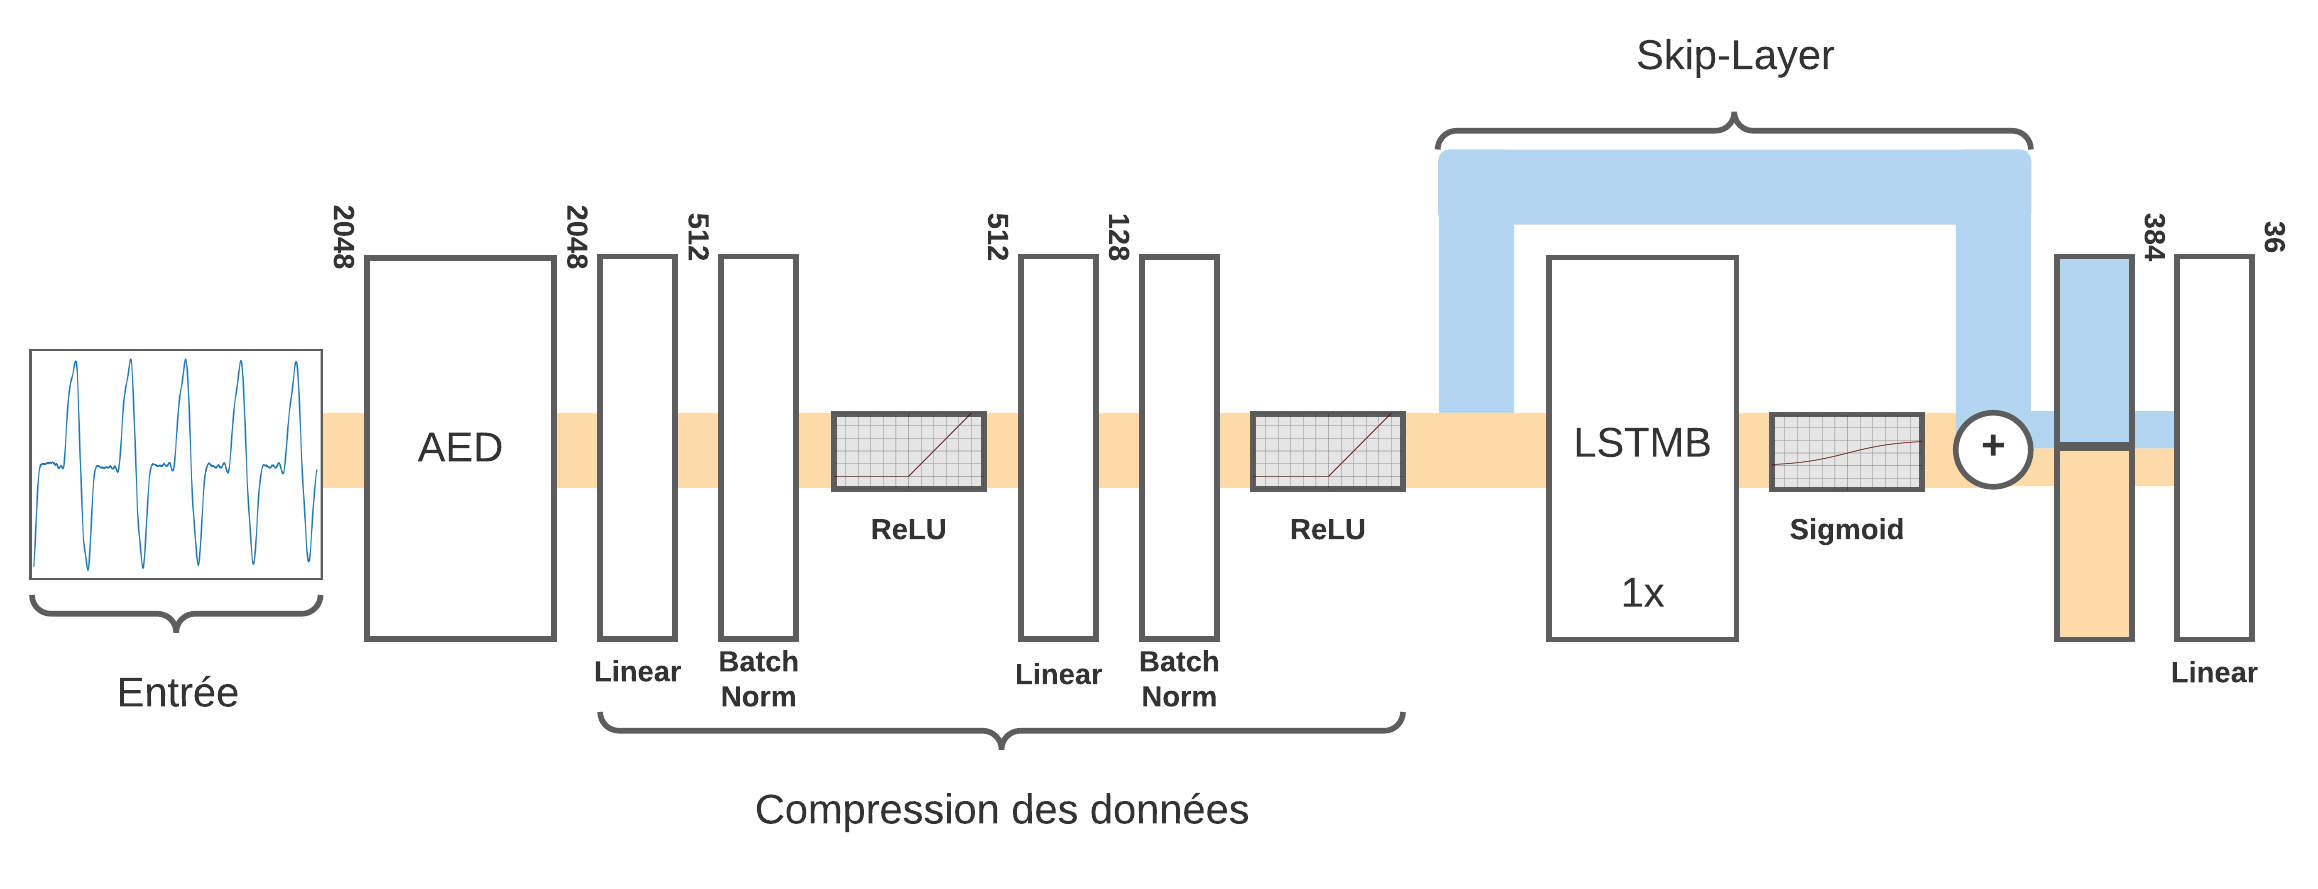
\includegraphics[width=1.1\linewidth,angle=-90,origin=c]{lstmb_no_fft}
\caption[]{Architecture LSTMB sans TFR. Source : Réalisé par \textsc{Küenzi} Jean-Daniel}
\label{fig:lstmb_no_fft}
\end{figure}

\section{Matrice de confusion sur l'ensemble de validation}

\begin{figure}[H]
\centering
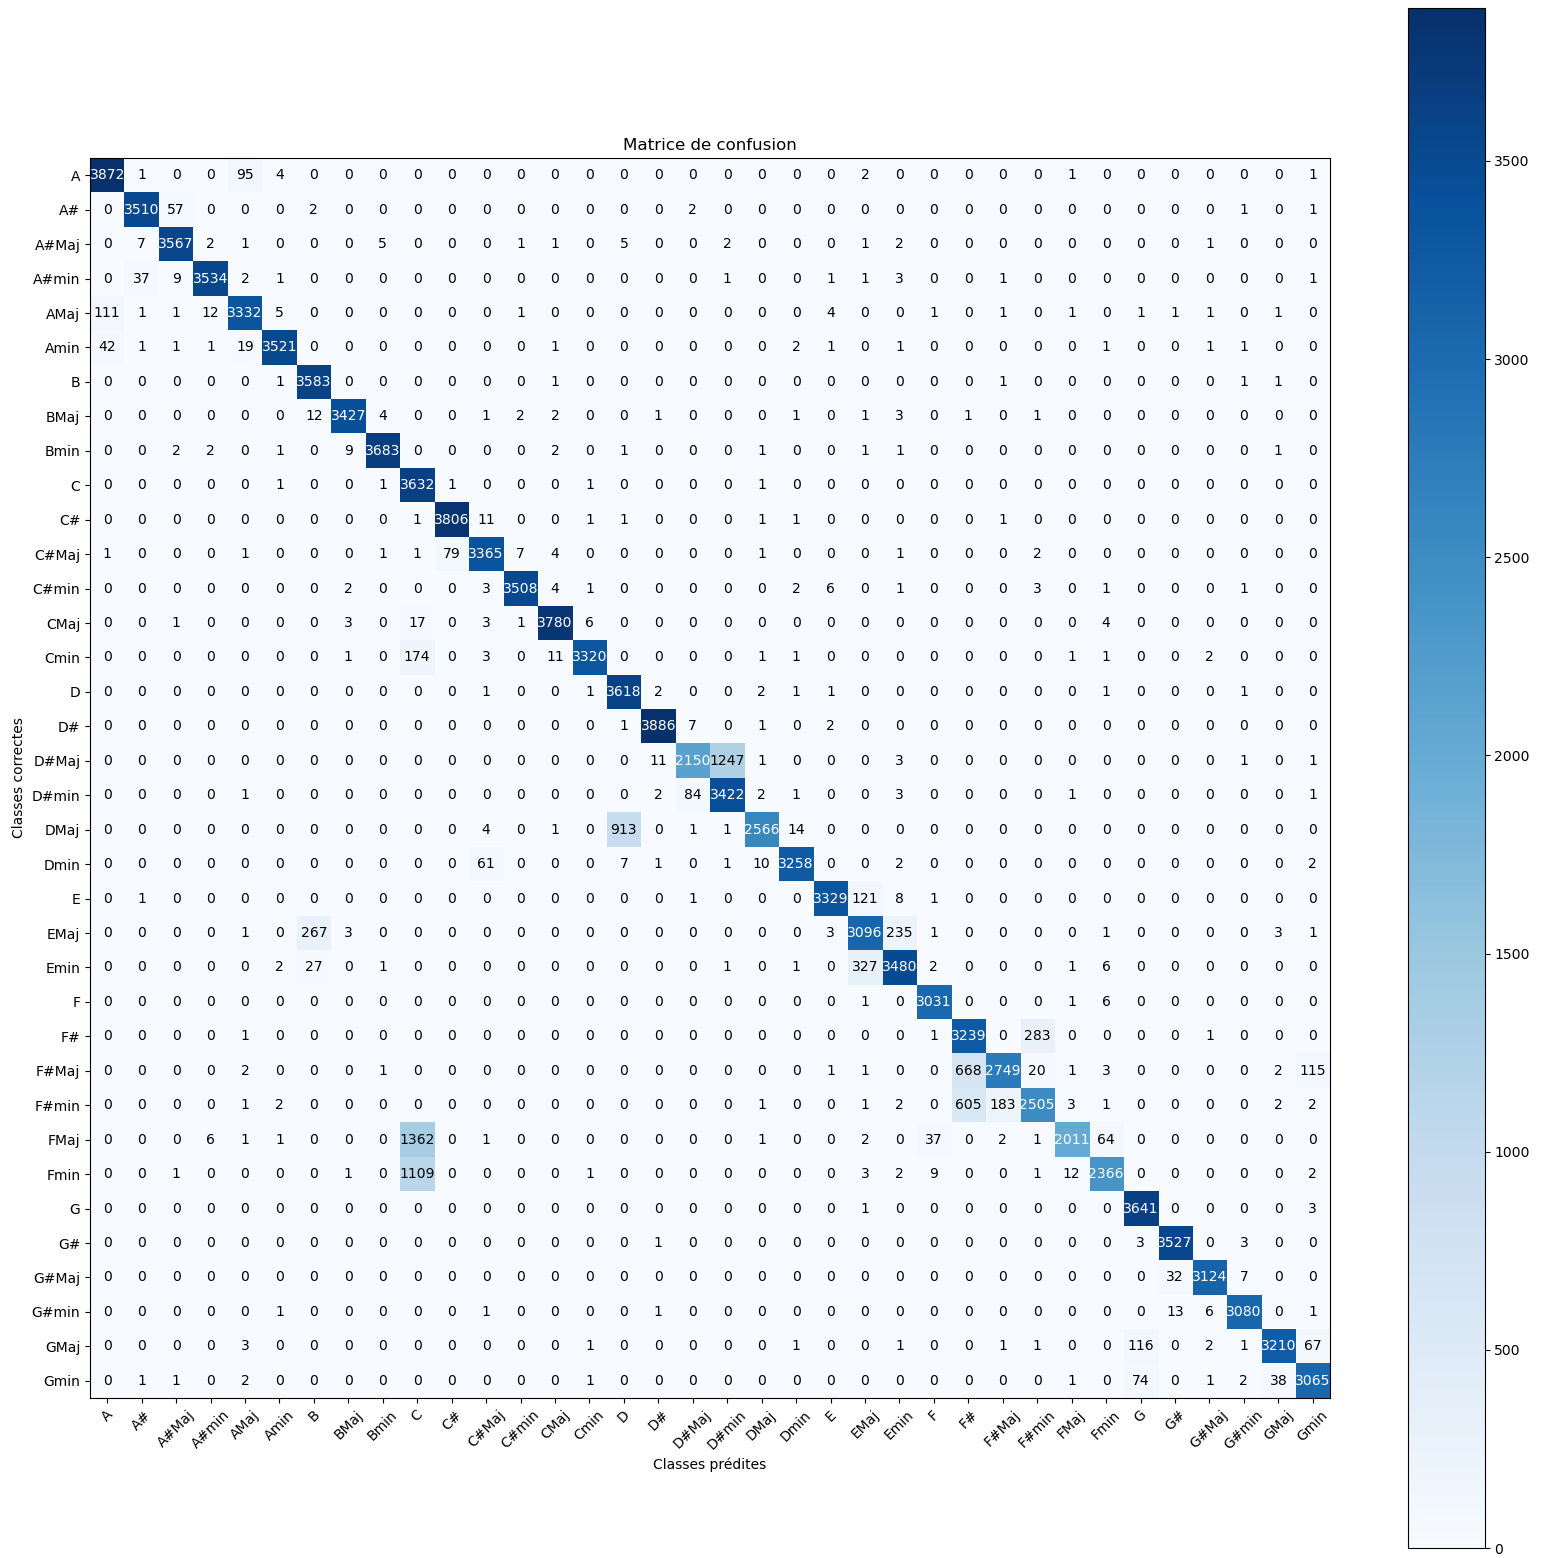
\includegraphics[width=1\linewidth]{cm_lstmb_no_fft}
\caption[]{Matrice de confusion pour l'architecture LSTMB sans TFR. Source : Réalisé par \textsc{Küenzi} Jean-Daniel}
\label{fig:cm_lstmb_no_fft}
\end{figure}	

\chapter{Annexe B : Architecture PMC sans TFR}
\label{app:2}

\section{Architecture}

\begin{figure}[H]
	\centering
	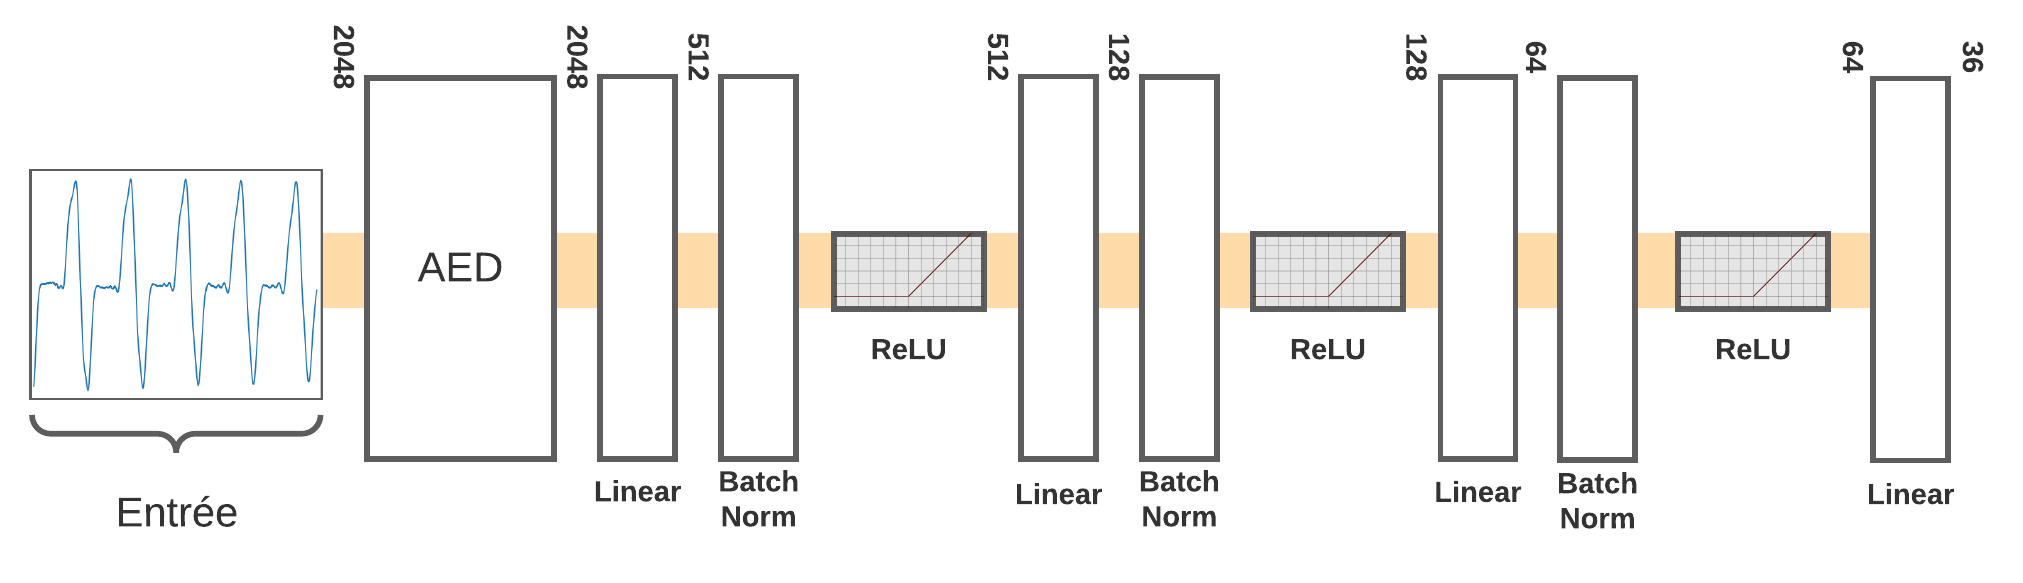
\includegraphics[width=1.1\linewidth,angle=-90,origin=c]{mlp_no_fft}
	\caption[]{Architecture PMC sans TFR. Source : Réalisé par \textsc{Küenzi} Jean-Daniel}
	\label{fig:mlp_no_fft}
\end{figure}

\section{Matrice de confusion sur l'ensemble de validation}

\begin{figure}[H]
\centering
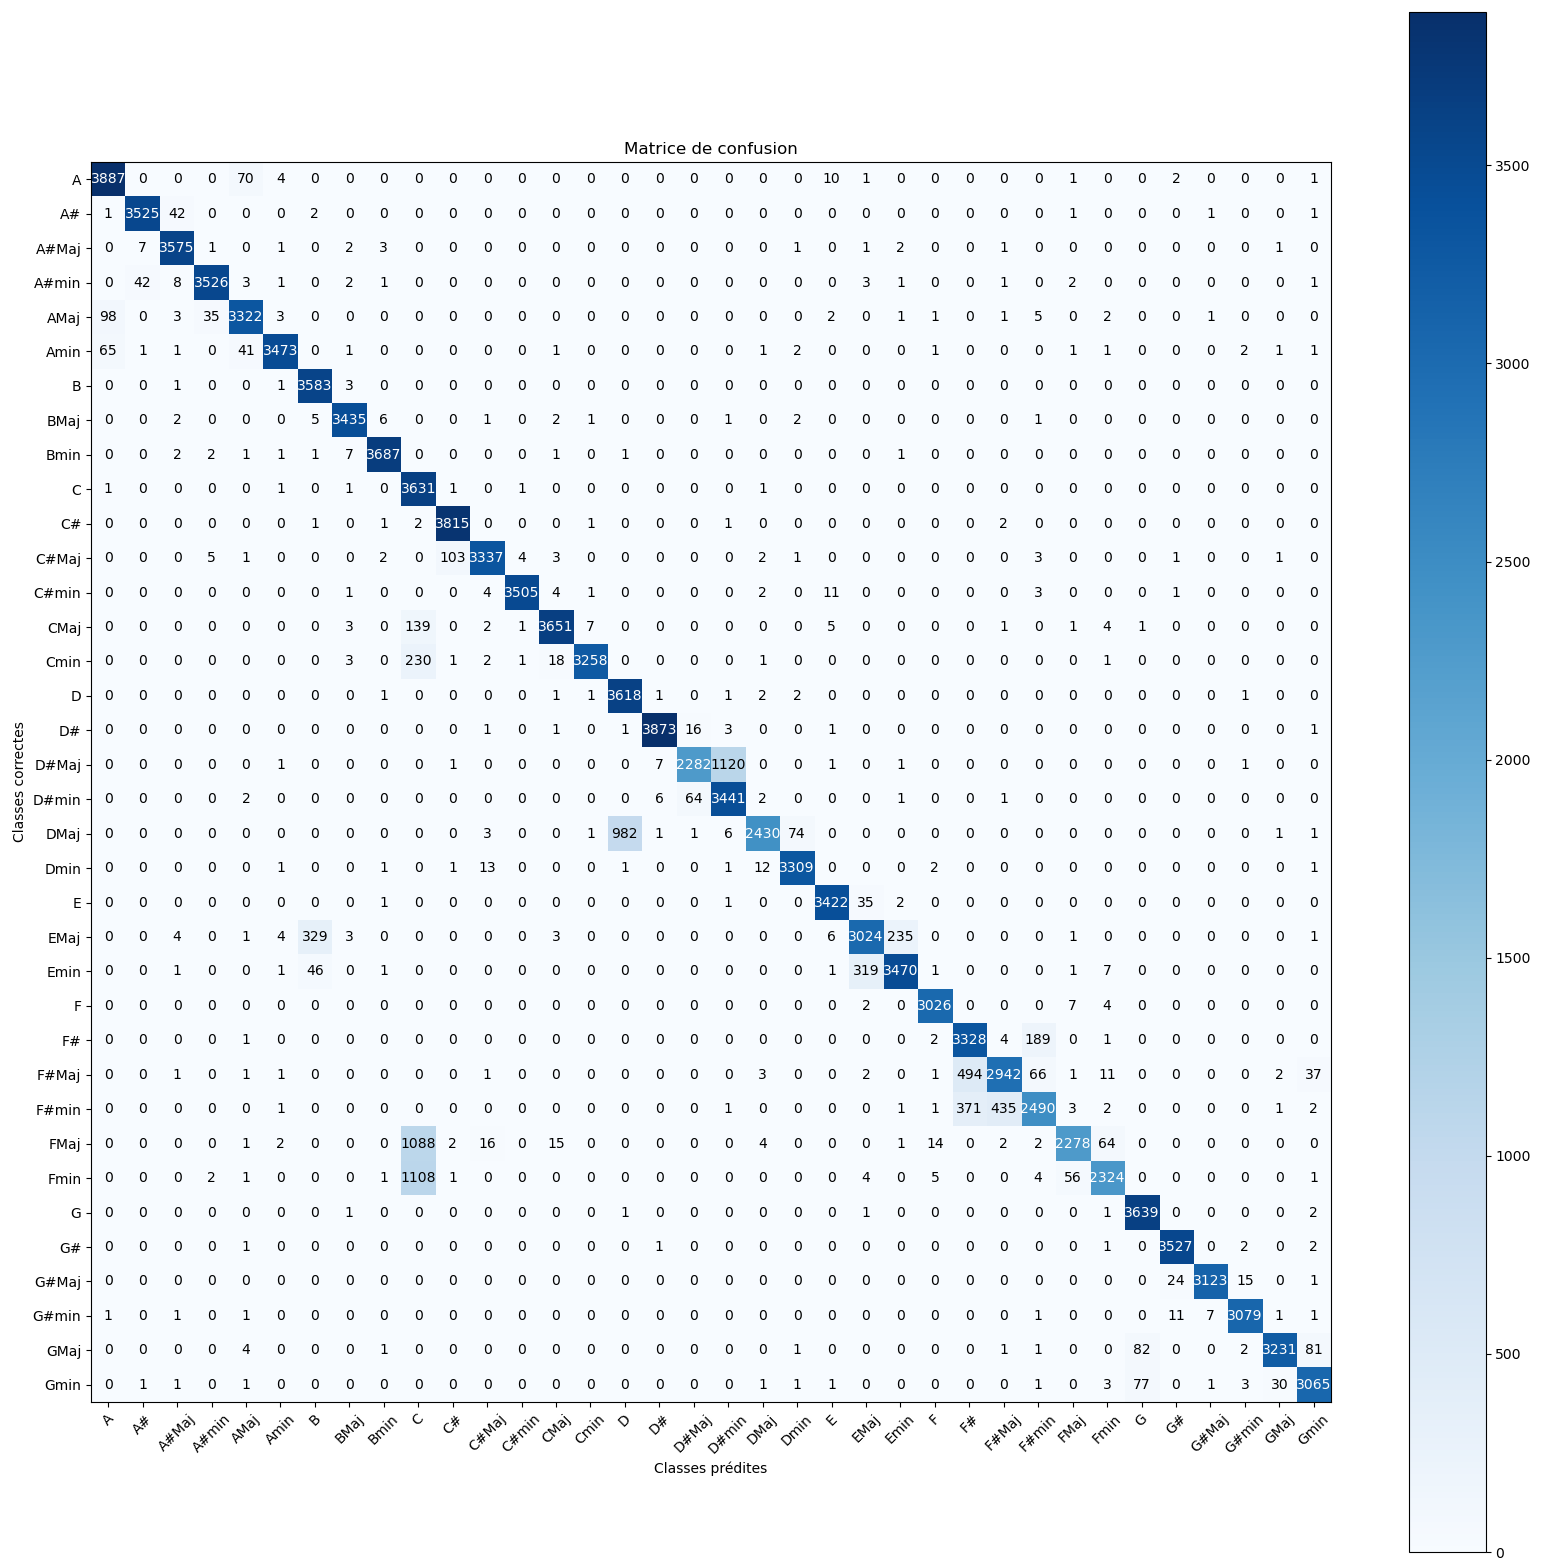
\includegraphics[width=1\linewidth]{cm_mlp_no_fft}
\caption[]{Matrice de confusion pour l'architecture PMC sans TFR. Source : Réalisé par \textsc{Küenzi} Jean-Daniel}
\label{fig:cm_mlp_no_fft}
\end{figure}	

\chapter{Annexe C : Architecture RNC sans TFR}
\label{app:3}

\section{Architecture}

\begin{figure}[H]
	\centering
	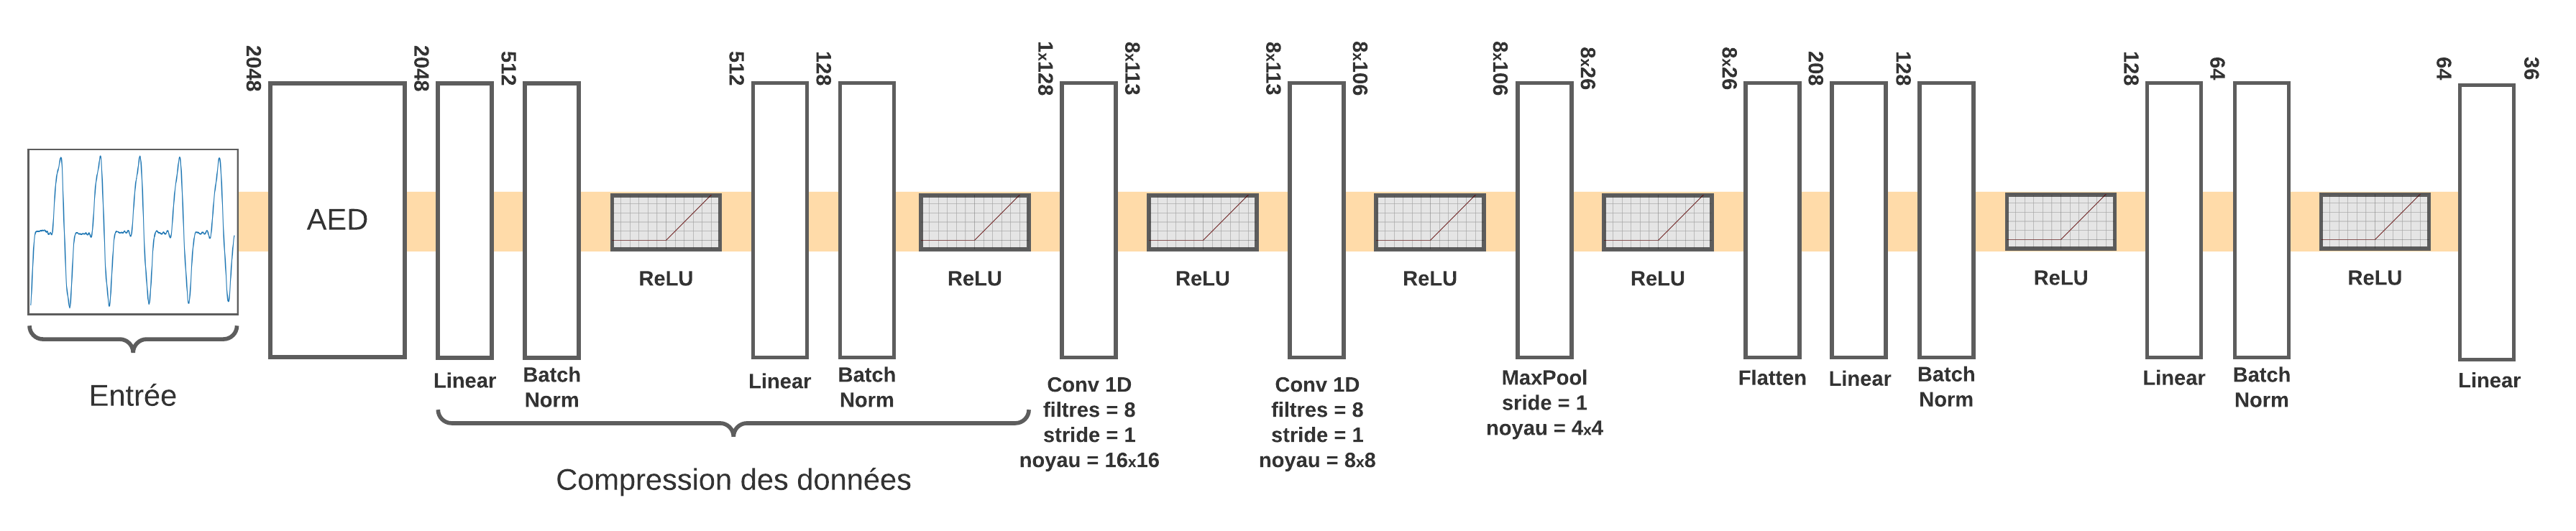
\includegraphics[width=1.1\linewidth,angle=-90,origin=c]{cnn_no_fft}
	\caption[]{Architecture RNC sans TFR. Source : Réalisé par \textsc{Küenzi} Jean-Daniel}
	\label{fig:cnn_no_fft}
\end{figure}

\section{Matrice de confusion sur l'ensemble de validation}

\begin{figure}[H]
\centering
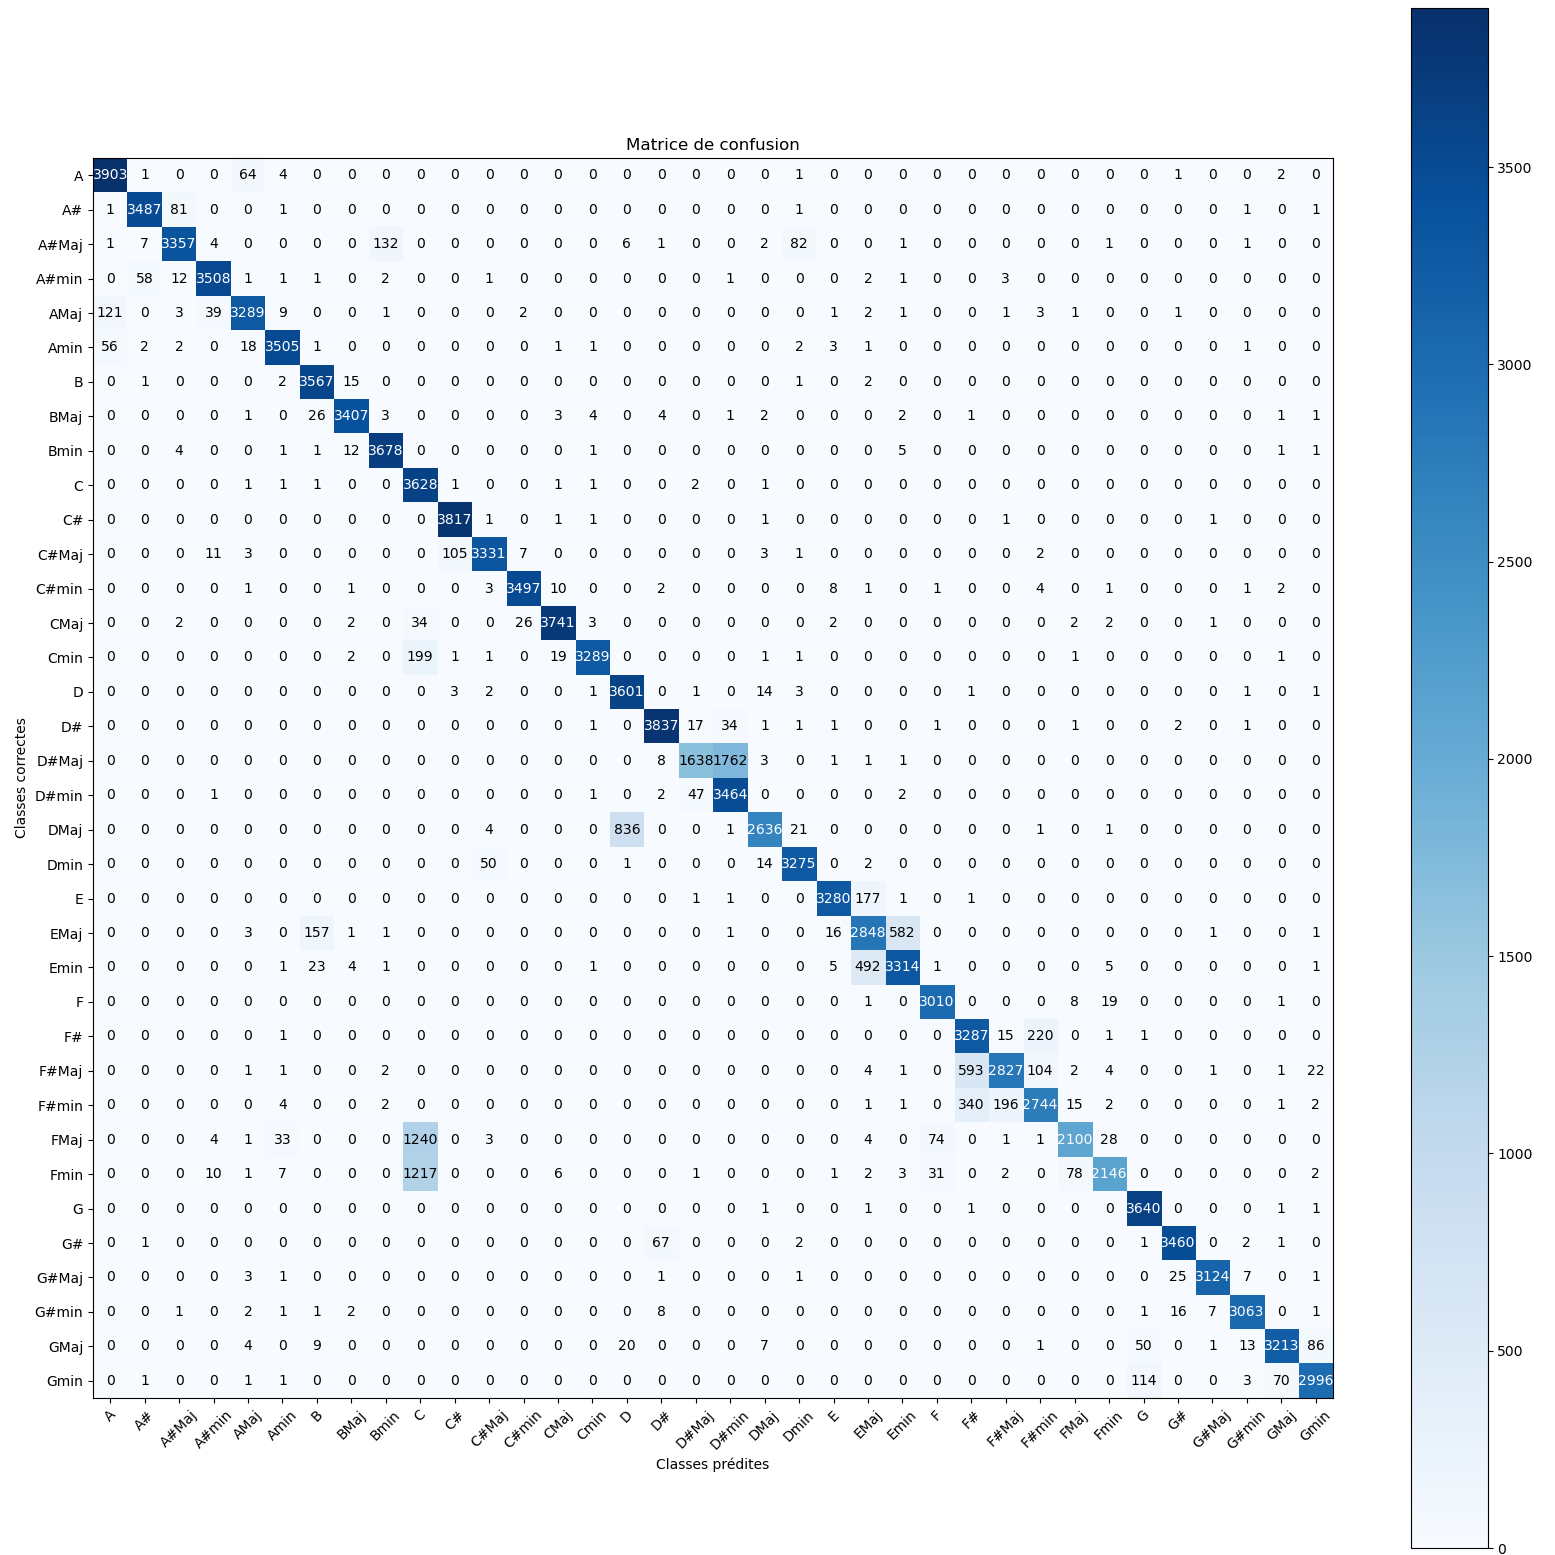
\includegraphics[width=1\linewidth]{cm_cnn_no_fft}
\caption[]{Matrice de confusion pour l'architecture RNC sans TFR. Source : Réalisé par \textsc{Küenzi} Jean-Daniel}
\label{fig:cm_cnn_no_fft}
\end{figure}

\chapter{Annexe D : Prédiciton de l'architecture PMC sur le fichier FMaj2 de l'ensemble de validation}
\label{app:4}

\begin{figure}[H]
	\centering
	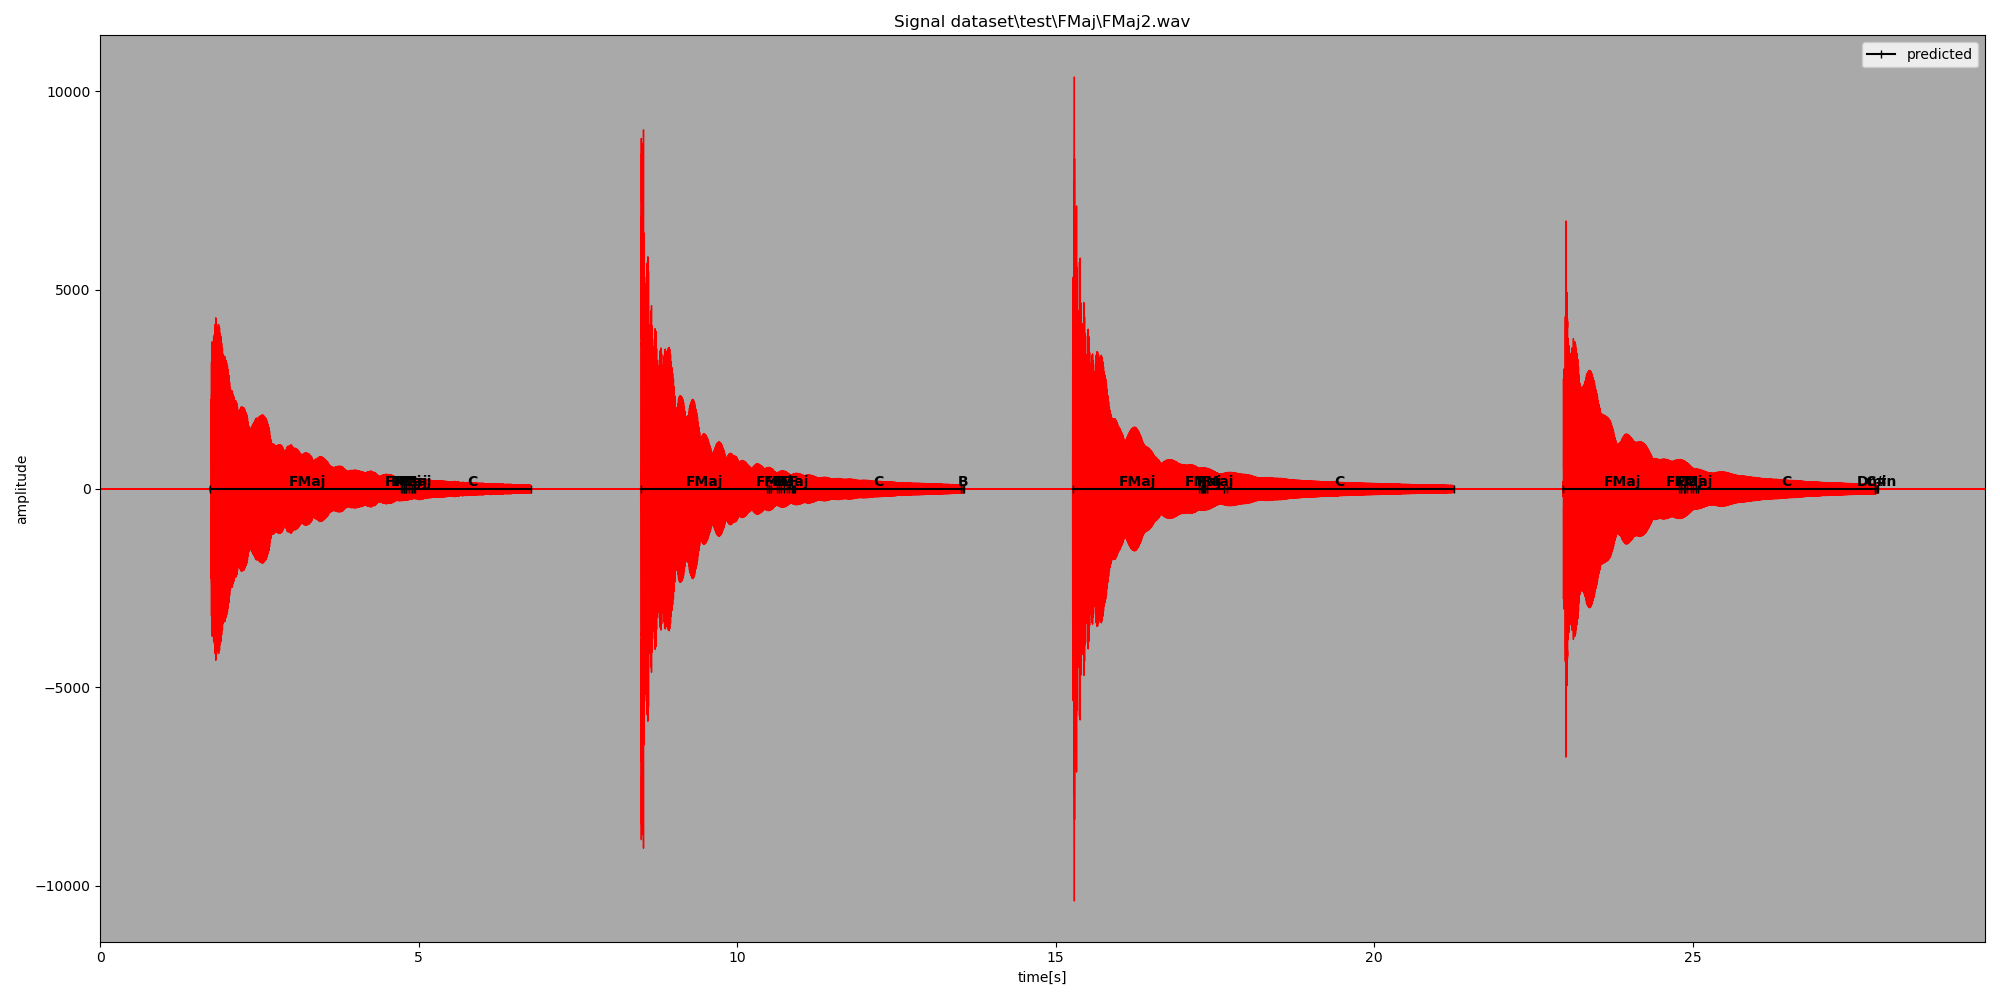
\includegraphics[width=1.2\linewidth,angle=-90,origin=c]{predict_FMaj2}
	\caption[]{Prédiction de l'architecture PMC sur le fichier FMaj2.wav du dataset de test. Source : Réalisé par \textsc{Küenzi} Jean-Daniel}
	\label{fig:predict_FMaj2}
\end{figure}

\chapter{Annexe E : Comparaison du spectre de Fourier de C\sh Maj et Dmin dans la même octave}
\label{app:5}

\begin{figure}[H]
	\centering
	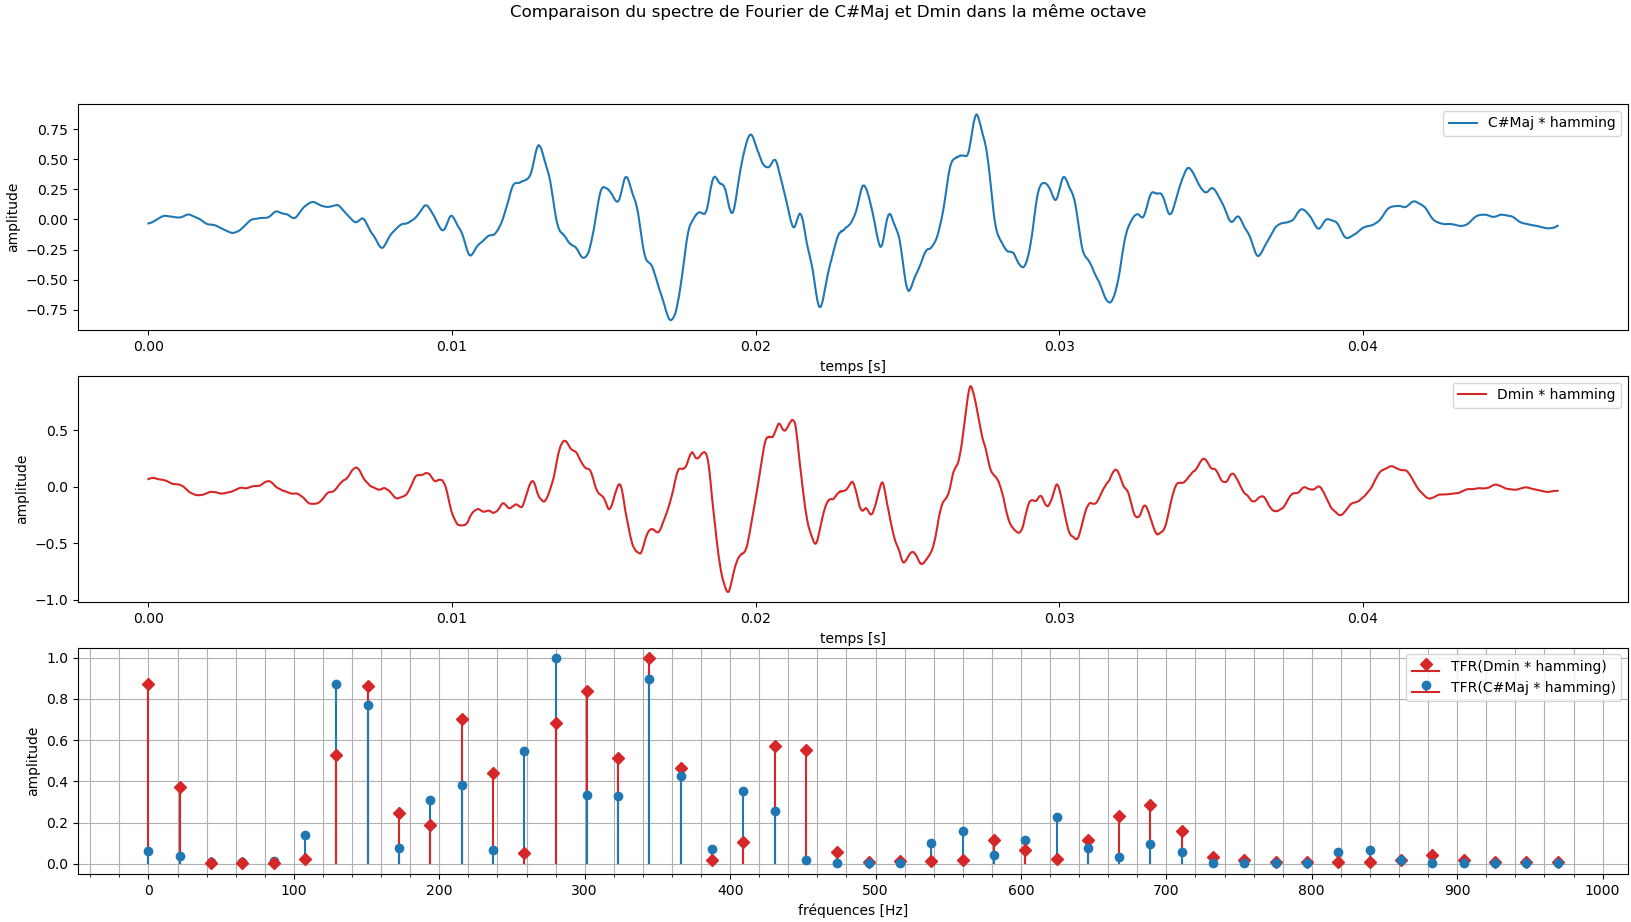
\includegraphics[width=1\linewidth]{fft_comp_chords_diff}
	\caption[]{Comparaison du spectre de Fourier de C\sh Maj et Dmin dans la même octave. Source : Réalisé par \textsc{Küenzi} Jean-Daniel}
	\label{fig:fft_comp_chords_diff}
\end{figure}

%%% COMMENT THESES LINES IF YOU DO NOT USE DEDICATED TOC FOR ANNEXES
\stopcontents[annexes]
\resumecontents[default]
%%% /COMMENT THESES LINES IF YOU DO NOT USE DEDICATED TOC FOR ANNEXES
\end{appendices}
%% !TeX spellcheck = fr_FR
\phantomsection
\addcontentsline{toc}{chapter}{Références documentaires}
%\bibliographystyle{plain}
\printbibliography[title={Référencess documentaires}]

\noindent\textit{Sites Web consultés – Code repris d’ailleurs – Notices techniques – Articles de presse – Ouvrage imprimés – Ouvrages électroniques – Chapitre dans un ouvrage imprimé – Rapports imprimés – Travaux universitaires – Articles de revues imprimés – Articles de périodiques électroniques – Communication dans un congrès. Pour chacun de ces types de document, les mise en forme sont dans le document « Méthode de citation et de rédaction d’une bibliographie ».}\\

\textit{Afin de gagner du temps, pensez à utiliser le logiciel de gestion bibliographique Zotero (et/ou BibTeX si vous utilisez LaTeX) pour la mise en forme et l’édition automatique de vos références à la norme ISO690.}
\cleardoublepage
\phantomsection
\addcontentsline{toc}{chapter}{Références documentaires}
%\bibliographystyle{plain}
\printbibliography[title={Références documentaires}]

\end{spacing}
\end{document}
%%%%%%%%%%%%%%%%%%%%%%%%%%%%%%%%%% DOCUMENT ENDS HERE %%%%%%%%%%%%%%%%%%%%%%%%%%
